\chapter{ÉTUDE DU ROBOT TANDEM}

Ce chapitre applique au robot Tandem les concepts théoriques des chapitres précédents. Il présente l'architecture du robot et ses contraintes mécaniques, puis la chaîne de traitement en quatre macro-blocs. Il détaille ensuite la campagne de tests qui dimensionne l'algorithme NSGA-II, avant d'exposer les résultats sur deux tailles de grille et l'effet de la couverture de la zone de travail sur le temps et l'énergie.

\section{Architecture et modélisation du robot Tandem}

\subsection{Présentation du robot et de la charge utile}

Le robot Tandem est un robot parallèle à câbles (CDPR) à 8 câbles, pleinement contraint en statique : il dispose de 6 degrés de liberté (3 forces et 3 moments). La trajectoire est planifiée en translation pure et l'orientation de la plateforme reste fixe ($\mathbf{R}=\mathbf{I}$). Selon la classification du chapitre~I, le robot est redondant :
\begin{itemize}
\item en 6~DDL : $m = 8 > n+1 = 7$ ;
\item en 3~DDL de translation : $m = 8 > n+1 = 4$.
\end{itemize}
Cette redondance de deux câbles offre plusieurs distributions de tension pour une même pose et aide à maintenir des tensions positives. Elle ne garantit pas à elle seule l'existence d'une solution mécanique : la faisabilité doit être vérifiée à chaque position, sous contraintes.

\begin{figure}[H]
\centering
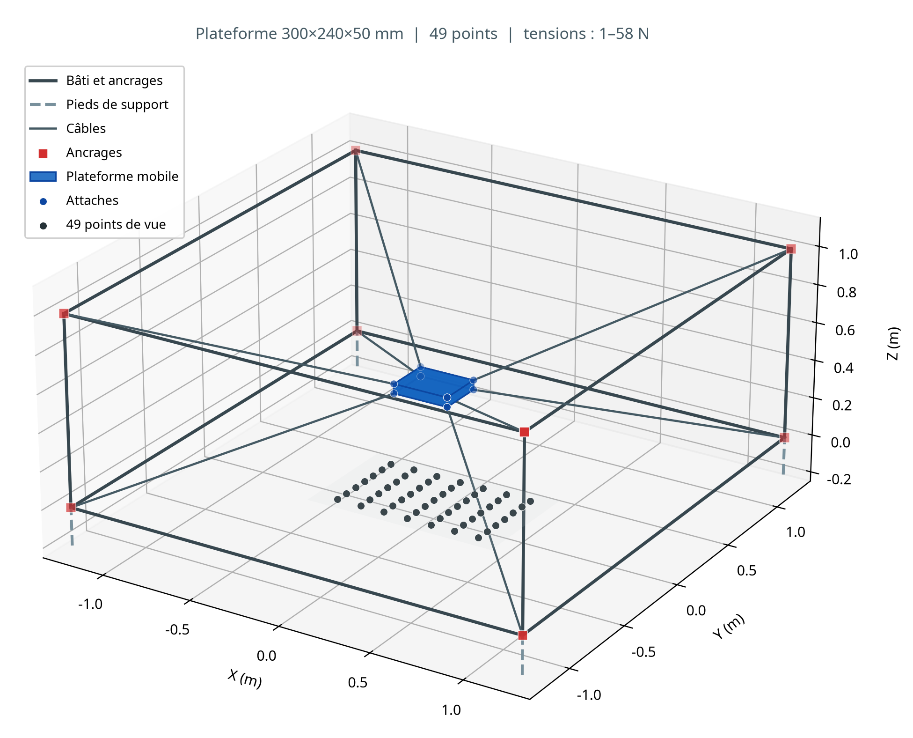
\includegraphics[width=0.92\textwidth,height=0.55\textheight,keepaspectratio]{robot_tandem_fig.png}
\caption{Robot Tandem}
\label{fig:robot_tandem}
\end{figure}

La plateforme est un cadre rigide en aluminium 6061-T6 qui porte les 8 points d'attache des câbles et la charge utile (module caméra Raspberry~Pi et électronique de contrôle). La caméra est orientée en vue nadir (verticale) et fixée sous la plateforme, conformément au protocole défini avec le SP3.

\begin{table}[H]
\centering
\caption{Caractéristiques de la plateforme mobile}
\label{tab:plateforme}
\begin{tabular}{|p{4.5cm}|p{5.5cm}|p{3.5cm}|}
\hline
\textbf{Paramètre} & \textbf{Valeur} & \textbf{Origine} \\
\hline
Matériau & Aluminium 6061-T6 & Choix de conception \\
\hline
Dimensions & $300 \times 240$~mm (ratio d'aspect 1,25) & Choix de conception \\
\hline
Masse à vide & $\approx 242$~g & Mesure \\
\hline
Charge utile & $\approx 114$~g & Somme des composants \\
\hline
Marge câblage et fixations & 8~\% & Hypothèse \\
\hline
Masse opérationnelle & 384~g & Calcul avec marge \\
\hline
Points d'attache & 8 & Choix de conception \\
\hline
\end{tabular}
\end{table}

\begin{table}[H]
\centering
\caption{Composition de la charge utile}
\label{tab:charge}
\begin{tabular}{|p{5.5cm}|p{2.2cm}|p{5.5cm}|}
\hline
\textbf{Composant} & \textbf{Masse} & \textbf{Rôle} \\
\hline
Raspberry Pi Zero 2 W & 11~g & Unité de calcul \\
\hline
Pi Camera Module 3 & 4,3~g & Capteur d'image RGB \\
\hline
Câble nappe CSI & 5~g & Liaison caméra et Pi \\
\hline
Cellule 18650 avec porte-pile & 47~g & Alimentation \\
\hline
Convertisseur (boost) & 12~g & Conversion 3,7~V vers 5~V \\
\hline
Capteur HC-SR04 & 5~g & Distance aux plants \\
\hline
Accéléromètre 3 axes & 10~g & Vérification de la stabilité \\
\hline
Boîtier de protection & 20~g & Protection \\
\hline
Total & $\approx 114$~g & \\
\hline
\end{tabular}
\end{table}

La masse à vide (242~g) et la charge utile ($\approx 114$~g) donnent environ 356~g. Avec la marge de 8~\% pour le câblage et les fixations, on obtient la masse opérationnelle de 384~g. C'est elle, et non la masse à vide, qui est utilisée dans tous les calculs mécaniques.

\subsection{Modèle géométrique inverse et contraintes}

Le modèle géométrique inverse (MGI) calcule la longueur de chaque câble à partir de la position $\mathbf{p}$ de la plateforme. L'orientation étant fixe, le calcul se réduit à une distance euclidienne entre l'ancrage $\mathbf{A}_i$ et l'attache $\mathbf{B}_i(\mathbf{p}) = \mathbf{p} + \mathbf{b}_i$ :
\begin{equation}
l_i = \sqrt{(A_{ix}-B_{ix}(\mathbf{p}))^2 + (A_{iy}-B_{iy}(\mathbf{p}))^2 + (A_{iz}-B_{iz}(\mathbf{p}))^2}
\label{eq:mgi}
\end{equation}
Les coordonnées des ancrages et des attaches sont définies dans la configuration de référence. Les câbles 1 à 4 sont les câbles hauts (ancrages à $z=1{,}00$~m) et les câbles 5 à 8 les câbles bas (ancrages à $z=0$).

La plateforme est évaluée à la hauteur de référence $z = 0{,}45$~m dans le repère fixe. Cette hauteur découle de la mission : distance opérationnelle capteur--plants de 0,30~m, hauteur de plants de 0,35~m et décalage sol/repère de 0,20~m.

\paragraph{Application numérique.}
Pour $\mathbf{p}=(0,\,0,\,0{,}45)$~m et $\mathbf{b}_i = (\pm 0{,}150;\,\pm 0{,}120;\,\pm 0{,}025)$~m :
\begin{equation}
\mathbf{B}_1 = (-0{,}150;\,0{,}120;\,0{,}475),\quad
l_1 = \sqrt{2{,}7625} \approx 1{,}662~\text{m}
\label{eq:l1}
\end{equation}
\begin{equation}
\mathbf{B}_5 = (-0{,}150;\,0{,}120;\,0{,}425),\quad
l_5 \approx 1{,}633~\text{m}
\label{eq:l5}
\end{equation}
Les six autres câbles se déduisent par symétrie.

\begin{table}[H]
\centering
\caption{Longueurs de câbles à la position centrale}
\label{tab:longueurs}
\begin{tabular}{|c|c|c|c|}
\hline
\textbf{Câble} & \textbf{Longueur (m)} & \textbf{Câble} & \textbf{Longueur (m)} \\
\hline
1 & 1,662 & 5 & 1,633 \\
\hline
2 & 1,662 & 6 & 1,633 \\
\hline
3 & 1,662 & 7 & 1,633 \\
\hline
4 & 1,662 & 8 & 1,633 \\
\hline
\end{tabular}
\end{table}

Les câbles du haut sont plus longs d'environ 2,9~cm que ceux du bas. Le poids de la plateforme vaut :
\begin{equation}
\mathbf{F}_{ext} = (0,\,0,\,-mg,\,0,\,0,\,0),\qquad mg = 0{,}384 \times 9{,}81 \approx 3{,}77~\text{N}
\label{eq:poids}
\end{equation}

\subsection{Espace de travail faisable (WFW) et singularité}

L'espace de travail faisable en tension (WFW) est déterminé par un test de faisabilité en effort, résolu par programmation linéaire (solveur HiGHS) :
\begin{equation}
\min_{\mathbf{T}}\ \mathbf{0}^{\top}\mathbf{T}
\quad\text{s.c.}\quad
\mathbf{W}(\mathbf{p})\,\mathbf{T} = -\mathbf{F}_{ext},
\quad T_{\min}\le T_i \le T_{\max}
\label{eq:wfw_lp}
\end{equation}
La matrice de structure $\mathbf{W}(\mathbf{p})\in\mathbb{R}^{6\times 8}$ s'écrit :
\begin{equation}
\mathbf{W} = \bigl[\ \mathbf{U}_i \ ;\ \mathbf{B}_i\times\mathbf{U}_i\ \bigr]_{i=1..8},
\quad
\mathbf{U}_i=\frac{\mathbf{A}_i-\mathbf{B}_i}{|\mathbf{A}_i-\mathbf{B}_i|}
\label{eq:W}
\end{equation}

\paragraph{Application numérique : câble 1 au centre.}
\begin{equation}
\mathbf{U}_1 \approx (-0{,}662;\,0{,}680;\,0{,}316),\quad
\mathbf{m}_1 \approx (-0{,}285;\,-0{,}267;\,-0{,}023)
\label{eq:u1}
\end{equation}
Avec $T_{\mathrm{haut}}=58$~N et $T_{\mathrm{bas}}=1$~N :
\begin{equation}
\sum F_z \approx 73{,}3 - 1{,}04 = 72{,}3~\text{N}
\label{eq:fz}
\end{equation}
Cette valeur dépasse largement le poids de 3,77~N : il existe une infinité de distributions admissibles.

Avant de résoudre le LP, le test contrôle le rang de $\mathbf{W}$. Si $\operatorname{rang}(\mathbf{W})<6$, le point est infaisable. Pour une plateforme carrée, le moment de lacet est identiquement nul et le rang tombe à~5. Pour la plateforme rectangulaire $300\times240$~mm (ratio 1,25), le rang reste égal à~6. La condition pratique retenue est un ratio d'aspect $\ge 1{,}20$.

\subsection{Configuration de référence}

\begin{table}[H]
\centering
\caption{Paramètres mécaniques et contraintes de la configuration de référence}
\label{tab:ref}
\footnotesize
\begin{tabular}{|p{4.0cm}|p{2.0cm}|p{1.8cm}|p{5.5cm}|}
\hline
\textbf{Paramètre} & \textbf{Valeur} & \textbf{Unité} & \textbf{Origine ou justification} \\
\hline
Plateforme & $300 \times 240$ & mm & Ratio d'aspect $1{,}25 \ge 1{,}20$ \\
\hline
Masse opérationnelle & 0,384 & kg & Mesure et marge de 8~\% \\
\hline
Tension minimale $T_{\min}$ & 1,0 & N & 100~\% de couverture \\
\hline
Tension maximale $T_{\max}$ & 58,0 & N & Borne de dimensionnement \\
\hline
Bornes zone sécurisée, X & $\pm 0{,}40$ & m & Mode zero-loss \\
\hline
Bornes zone sécurisée, Y & $\pm 0{,}24$ & m & Mode zero-loss \\
\hline
Limites verticales Z & $[0\,;\,0{,}80]$ & m & Configuration historique \\
\hline
Hauteur de référence & 0,45 & m & Dans le repère fixe \\
\hline
Distance capteur--plants & 0,30 & m & Protocole SP3 \\
\hline
Vitesse maximale $v_{\max}$ & 0,045 & m/s & Hypothèse de conception \\
\hline
Accélération maximale $a_{\max}$ & 0,03 & m/s$^2$ & Hypothèse de conception \\
\hline
Temps de stabilisation & 2,0 & s/point & Évite le flou de mouvement \\
\hline
\end{tabular}
\end{table}

La borne $T_{\max}=58$~N suppose une réduction d'environ 5:1 sur un moteur NEMA~17. La fenêtre de service couvre des plants jusqu'à 0,50~m (haricot nain). Le mode zero-loss désigne une zone resserrée garantissant 100~\% de points faisables.

\section{Chaîne de traitement en quatre macro-blocs}
\label{sec:macro}

Le pipeline comprend douze sous-blocs regroupés en quatre macro-blocs. Cette modularité apporte testabilité, traçabilité et parallélisation.

\begin{figure}[H]
\centering
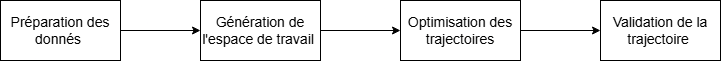
\includegraphics[width=0.95\textwidth,height=0.42\textheight,keepaspectratio]{macrobloc.png}
\caption{Chaîne de traitement en quatre macro-blocs}
\label{fig:macro}
\end{figure}

\begin{table}[H]
\centering
\caption{Correspondance des quatre macro-blocs}
\label{tab:macro}
\footnotesize
\begin{tabular}{|p{4.5cm}|p{4.0cm}|p{5.0cm}|}
\hline
\textbf{Macro-bloc} & \textbf{Rôle} & \textbf{Entrées et sorties} \\
\hline
1. Préparation des données & Paramètres, $\mathbf{W}$, MGI & Paramètres $\to$ configuration, $\mathbf{W}$ \\
\hline
2. Génération de l'espace de travail & Faisabilité, points retenus & Configuration $\to$ points filtrés \\
\hline
3. Optimisation des trajectoires & Matrice de coûts, ordre optimal & Points filtrés $\to$ solutions \\
\hline
4. Validation de la trajectoire & Profilage, vérification & Trajectoires $\to$ profils, rapport \\
\hline
\end{tabular}
\end{table}

\subsection{Préparation des données}

Le sous-bloc~0 centralise les paramètres dans une structure immuable après validation. Huit règles de validation lèvent une erreur explicite en cas de conflit.

\begin{figure}[H]
\centering
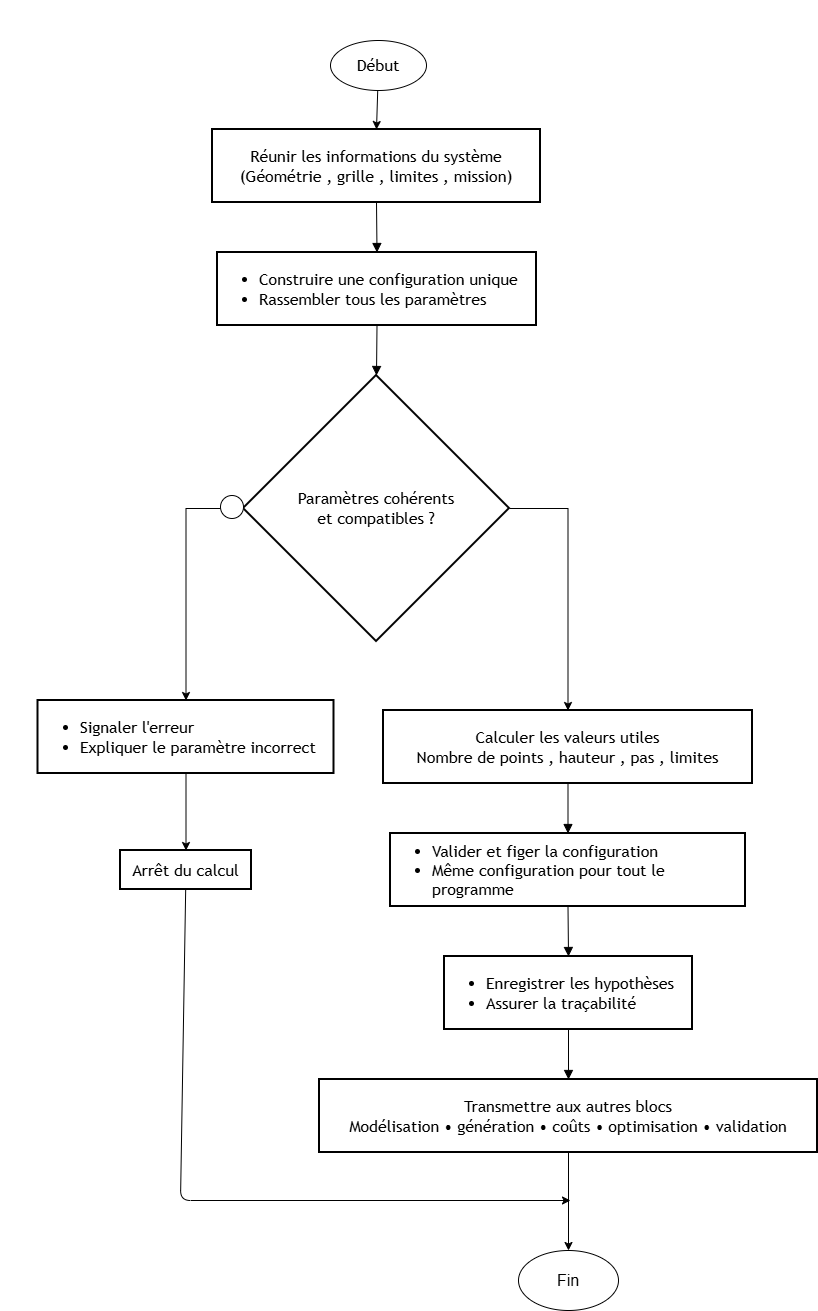
\includegraphics[width=0.95\textwidth,height=0.62\textheight,keepaspectratio]{bloc0.png}
\caption{Organigramme de la configuration}
\label{fig:bloc0}
\end{figure}

Le sous-bloc~1 construit $\mathbf{W}$ et le sous-bloc~2 assure la cinématique (MGI fermé, MGD par moindres carrés non linéaires).

\subsection{Génération de l'espace de travail}

Le sous-bloc~4 génère une grille centrée ; le sous-bloc~5 filtre par le test WFW précédé du test de rang. Le centre joue le rôle de verrou.

\clearpage
\begin{figure}[H]
\centering
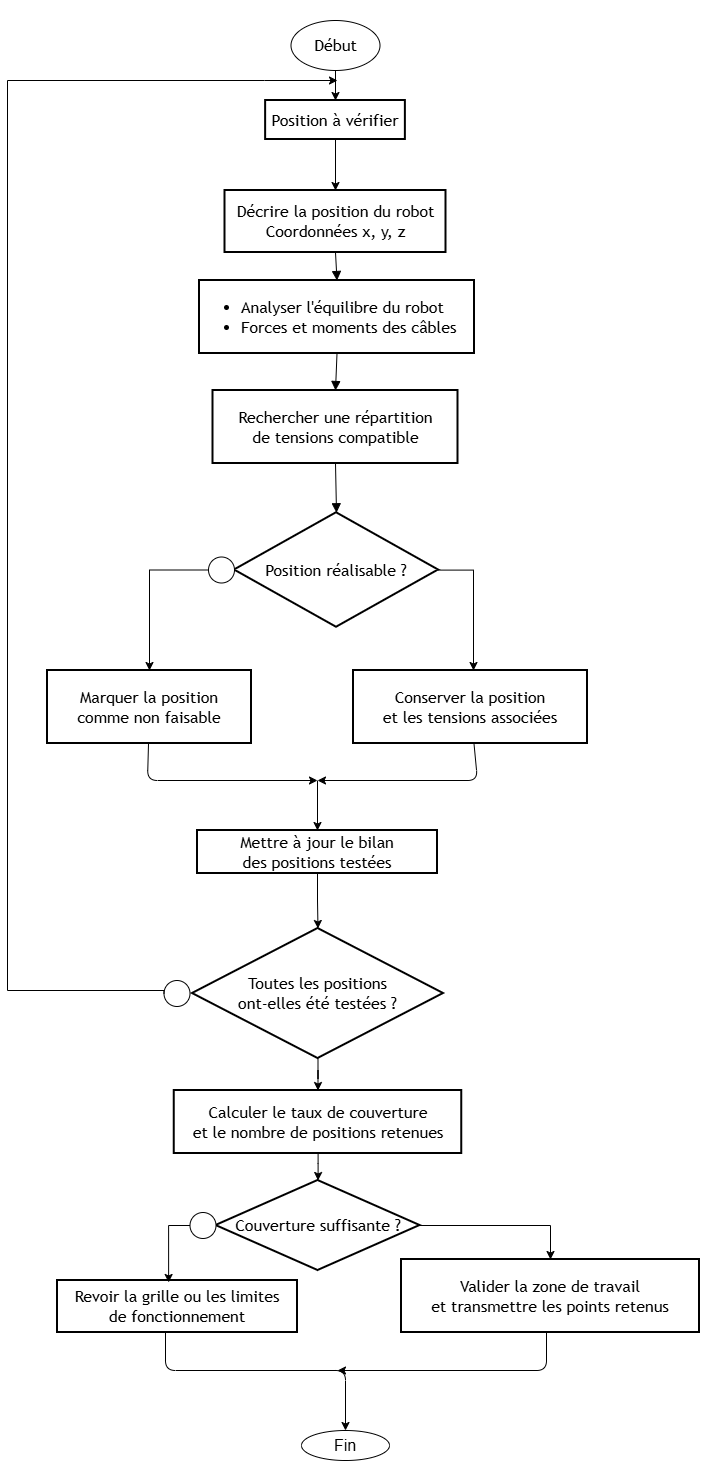
\includegraphics[width=\textwidth,height=0.90\textheight,keepaspectratio]{bloc3.png}
\caption{Organigramme du test WFW}
\label{fig:bloc3}
\end{figure}
\clearpage

\subsection{Optimisation des trajectoires}
\label{sec:macro3}

\begin{figure}[H]
\centering
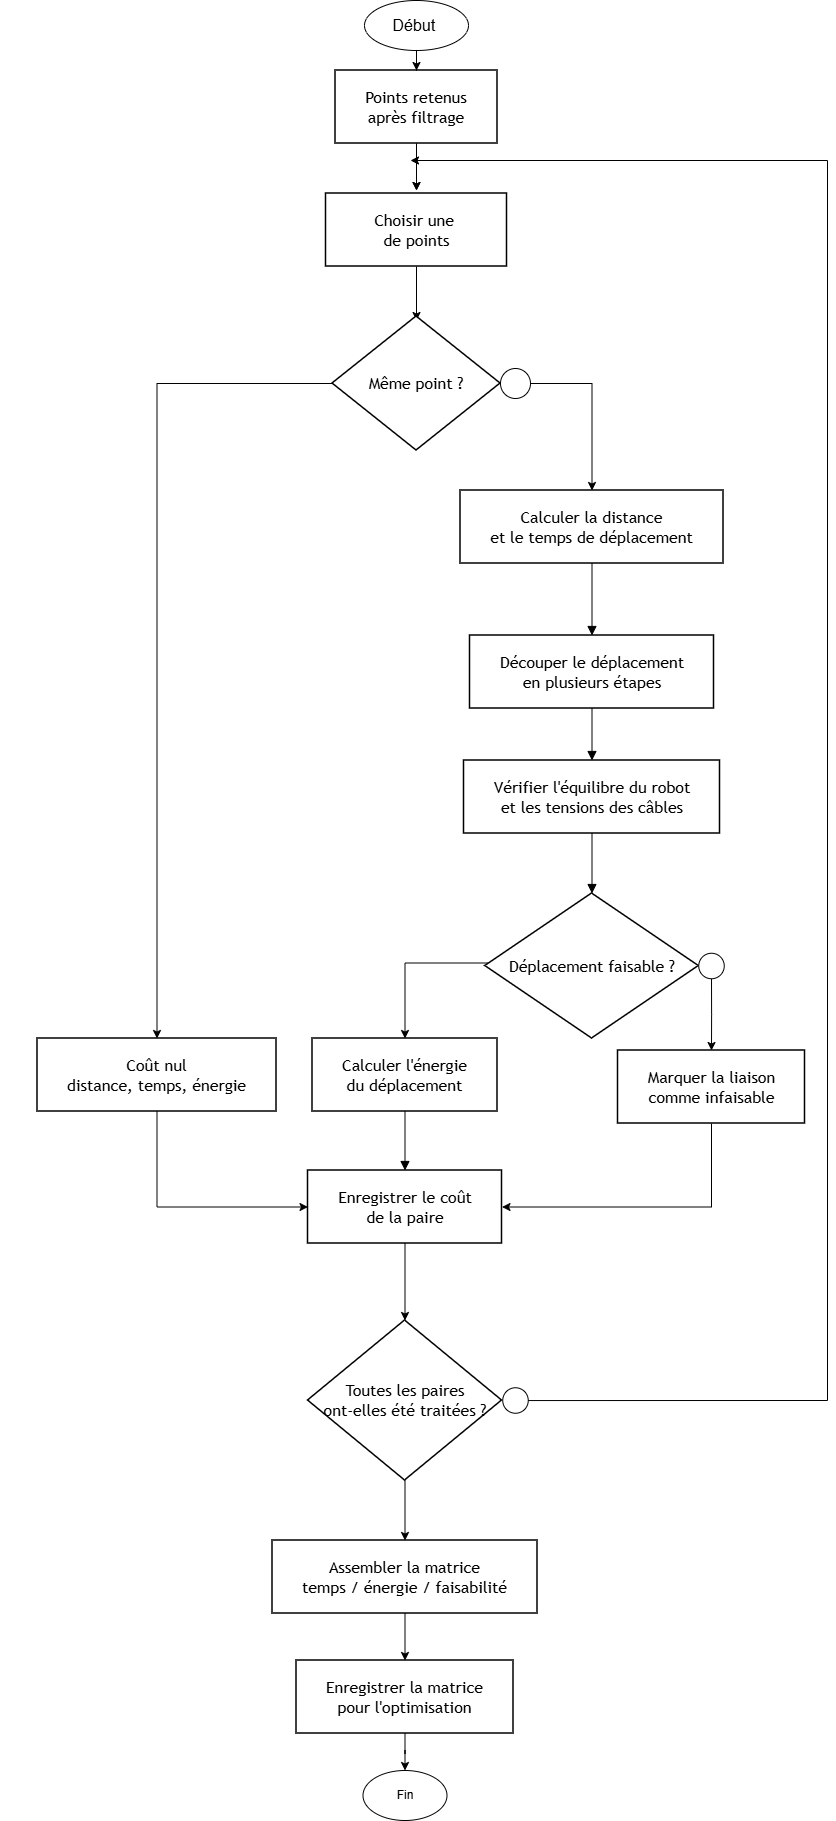
\includegraphics[width=\textwidth,height=0.82\textheight,keepaspectratio]{bloc6.png}
\caption{Organigramme du calcul de matrice de coût}
\label{fig:bloc6}
\end{figure}
\clearpage

Le temps de déplacement suit un profil LSPB :
\begin{equation}
d_{\mathrm{acc}}=\frac{v_{\max}^2}{2a_{\max}},\qquad d_{\mathrm{full}}=2\,d_{\mathrm{acc}}
\label{eq:dacc}
\end{equation}
Si $d\ge d_{\mathrm{full}}$, le profil est trapézoïdal ; sinon triangulaire. Avec $v_{\max}=0{,}045$~m/s et $a_{\max}=0{,}03$~m/s$^2$, $d_{\mathrm{acc}}\approx0{,}034$~m.

L'énergie est une estimation mécanique quasi-statique :
\begin{equation}
E\approx\sum_{k}\sum_{i=1}^{8}T_i\bigl(\mathbf{p}_k^{\mathrm{mid}}\bigr)\,|\Delta l_{i,k}|
\label{eq:energie}
\end{equation}
Les tensions sont obtenues par un QP à norme minimale, résolu d'abord par pseudo-inverse puis par SLSQP si nécessaire.

Un individu code une permutation des points non centraux. Les objectifs sont le temps et l'énergie totaux. Les contraintes sont gérées par pénalisation. NSGA-II utilise le croisement OX (taux 0,9) et la mutation par inversion (taux 0,1).

\subsection{Validation de la trajectoire}

Le sous-bloc~9 génère les profils LSPB ; le sous-bloc~10 contrôle sept invariants ; le sous-bloc~11 compare à une baseline. La mission suit six étapes : initialisation, déplacement, stabilisation 2~s, prise de vue, répétition, retour au centre.

\section{Préparation des données}

La campagne s'appuie sur une commande unique (grille, zero-loss, population, générations, graine~42). La graine rend l'optimisation déterministe. Pour la grille $7\times7$, le recouvrement entre points voisins assure une couverture complète de la parcelle.

\section{Génération de l'espace de travail}

\subsection{Zone sécurisée et frontière du WFW}

\begin{table}[H]
\centering
\caption{Synthèse de l'exploration de l'espace de travail}
\label{tab:wfw_synth}
\footnotesize
\begin{tabular}{|p{3.2cm}|c|c|c|c|c|}
\hline
\textbf{Configuration} & \textbf{Grille} & \textbf{Pas (m)} & \textbf{Bornes X/Y} & \textbf{Retenus} & \textbf{Taux} \\
\hline
Zone sécurisée & $7\times7$ & $0{,}133\times0{,}080$ & $\pm0{,}40/\pm0{,}24$ & 49/49 & 100~\% \\
\hline
Zone sécurisée & $9\times9$ & $0{,}100\times0{,}060$ & $\pm0{,}40/\pm0{,}24$ & 81/81 & 100~\% \\
\hline
Zone étendue & $7\times7$ & $0{,}150\times0{,}090$ & $\pm0{,}45/\pm0{,}27$ & 49/49 & 100~\% \\
\hline
Zone étendue & $9\times9$ & $0{,}150\times0{,}090$ & $\pm0{,}60/\pm0{,}36$ & 77/81 & 95,1~\% \\
\hline
\end{tabular}
\end{table}

\begin{figure}[H]
\centering
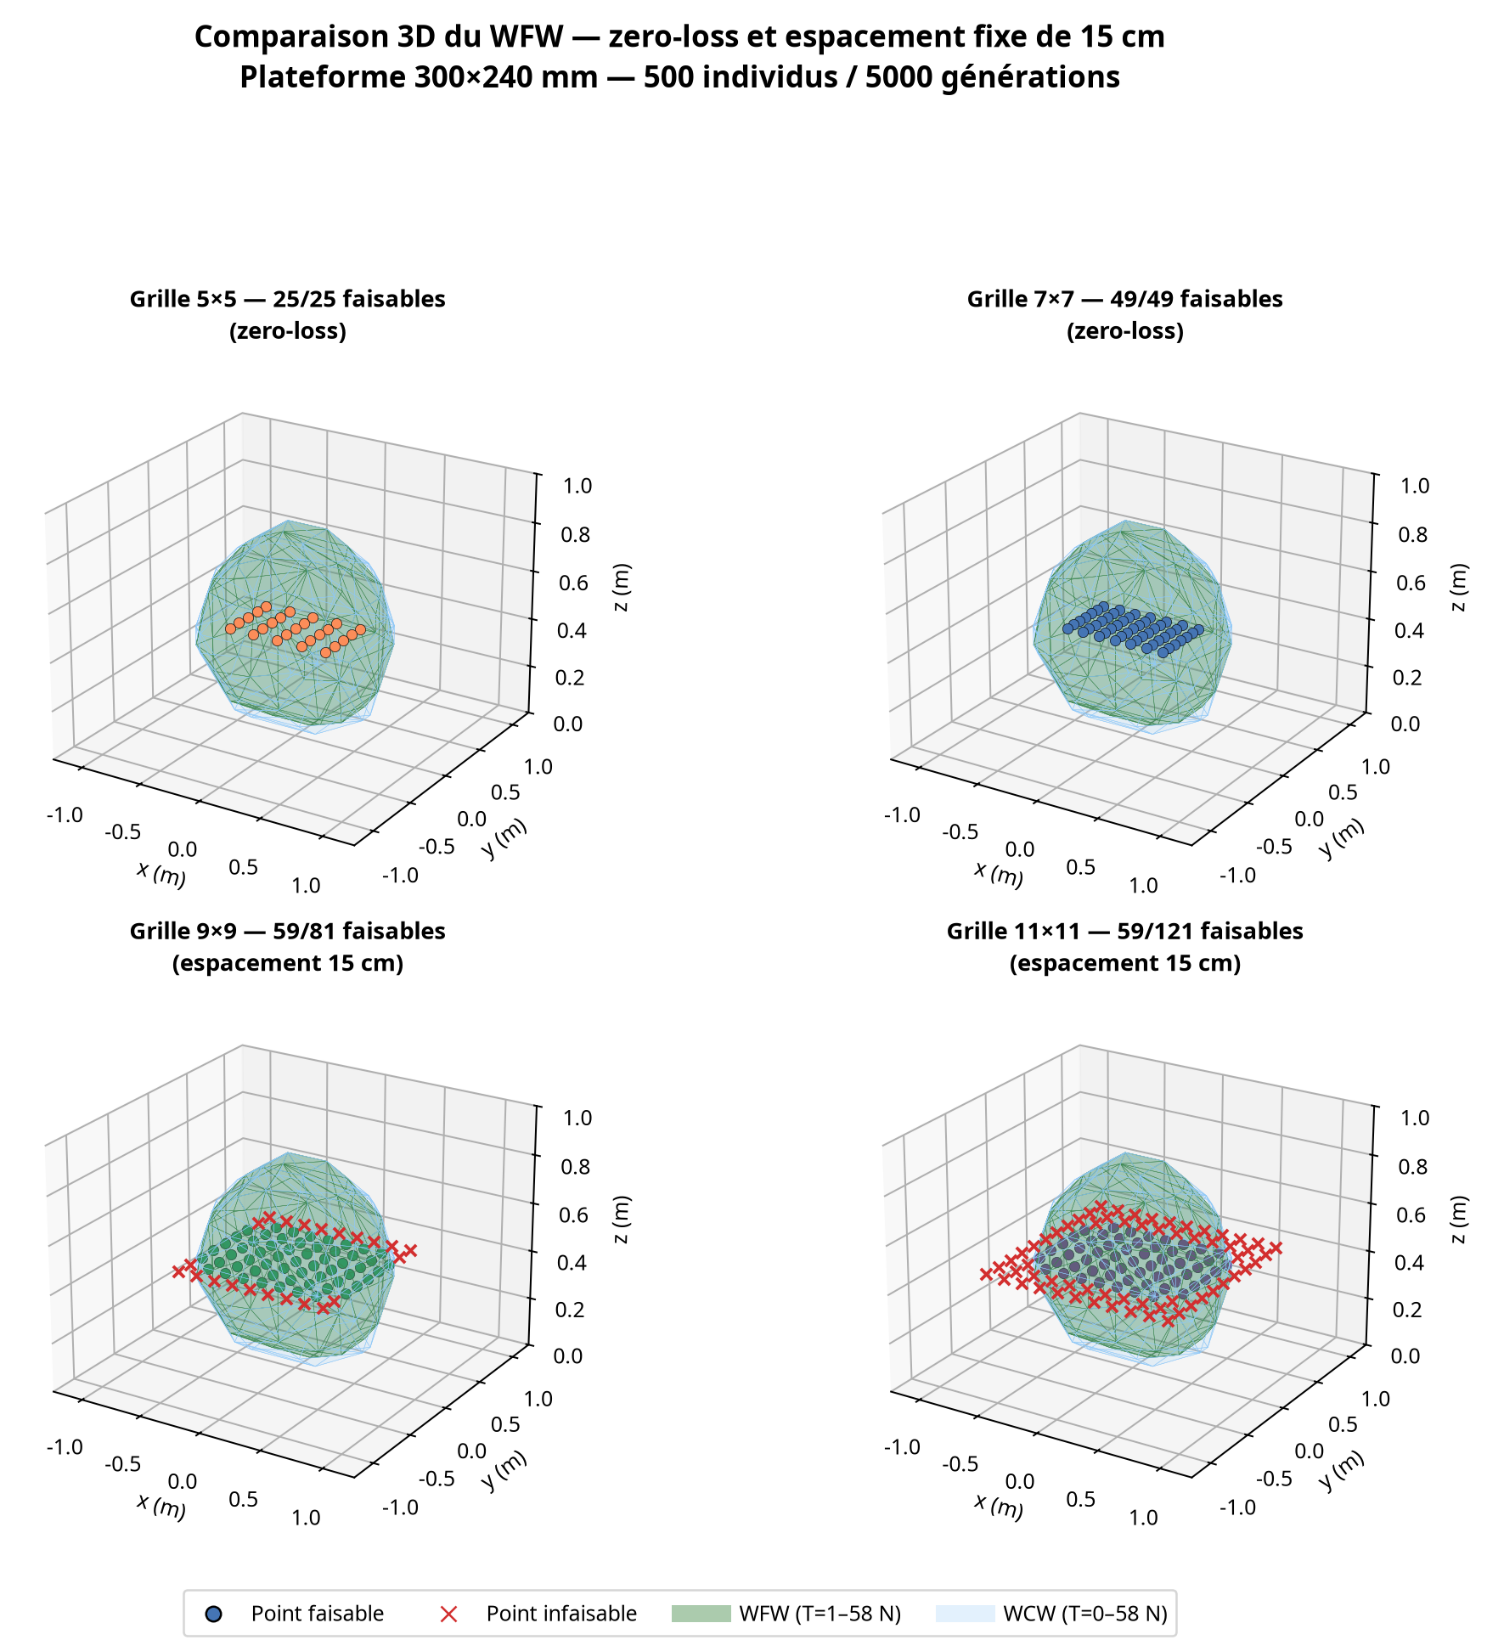
\includegraphics[width=0.95\textwidth,height=0.48\textheight,keepaspectratio]{wfw_grille.jpg}
\caption{WFW 3D et faisabilité des points selon la taille de grille}
\label{fig:wfw_grille}
\end{figure}

L'espace de travail faisable en effort (WFW) présente une forme sphérique tronquée dont les limites physiques rejettent les points situés aux extrémités de la grille (croix rouges). Ce comportement justifie le recours au mode «~zero-loss~» : pour garantir 100~\% de points viables, la zone de travail doit être volontairement restreinte.


\section{Optimisation des trajectoires : dimensionnement de NSGA-II}

Campagne de 50 exécutions (2 grilles $\times$ 5 populations $\times$ 5 générations), graine~42, complétée par 12 exécutions de robustesse (graines 30 et 100).

\begin{table}[H]
\centering
\caption{Grille $7\times7$ : temps (s) / énergie (J) du meilleur point, graine 42}
\label{tab:camp7}
\footnotesize
\begin{tabular}{|c|c|c|c|c|c|}
\hline
\textbf{Pop.} & \textbf{1500} & \textbf{2000} & \textbf{3000} & \textbf{4000} & \textbf{5000} \\
\hline
200 & 178,58 / 248,8 & 177,98 / 247,1 & 177,98 / 247,0 & 177,98 / 247,0 & 177,98 / 247,0 \\
\hline
300 & 177,30 / 246,4 & 177,30 / 246,4 & 177,30 / 246,4 & 177,30 / 246,4 & 177,30 / 246,4 \\
\hline
400 & 178,96 / 250,4 & 177,98 / 248,1 & 177,98 / 247,5 & 177,98 / 247,0 & 177,30 / 246,7 \\
\hline
500 & 177,30 / 246,4 & 177,30 / 246,4 & 177,30 / 246,4 & 177,30 / 246,4 & 177,30 / 246,4 \\
\hline
600 & 177,30 / 246,4 & 177,30 / 246,4 & 177,30 / 246,4 & 177,30 / 246,4 & 177,30 / 246,4 \\
\hline
\end{tabular}
\end{table}

\begin{table}[H]
\centering
\caption{Grille $9\times9$ : temps (s) / énergie (J) du meilleur point, graine 42}
\label{tab:camp9}
\footnotesize
\begin{tabular}{|c|c|c|c|c|c|}
\hline
\textbf{Pop.} & \textbf{1500} & \textbf{2000} & \textbf{3000} & \textbf{4000} & \textbf{5000} \\
\hline
200 & 267,17 / 325,4 & 262,20 / 318,8 & 255,64 / 307,4 & 254,90 / 304,3 & 253,65 / 304,3 \\
\hline
300 & 260,02 / 312,4 & 253,57 / 304,7 & 248,60 / 295,2 & 248,09 / 295,2 & 247,55 / 294,2 \\
\hline
400 & 262,77 / 315,6 & 253,77 / 304,3 & 252,06 / 301,7 & 249,98 / 299,0 & 249,98 / 297,9 \\
\hline
500 & 248,09 / 296,6 & 248,09 / 296,6 & 247,55 / 295,6 & 247,04 / 295,4 & 247,04 / 294,8 \\
\hline
600 & 255,44 / 310,2 & 253,90 / 305,5 & 249,81 / 298,0 & 247,78 / 294,1 & 247,04 / 294,1 \\
\hline
\end{tabular}
\end{table}

\begin{figure}[H]
\centering
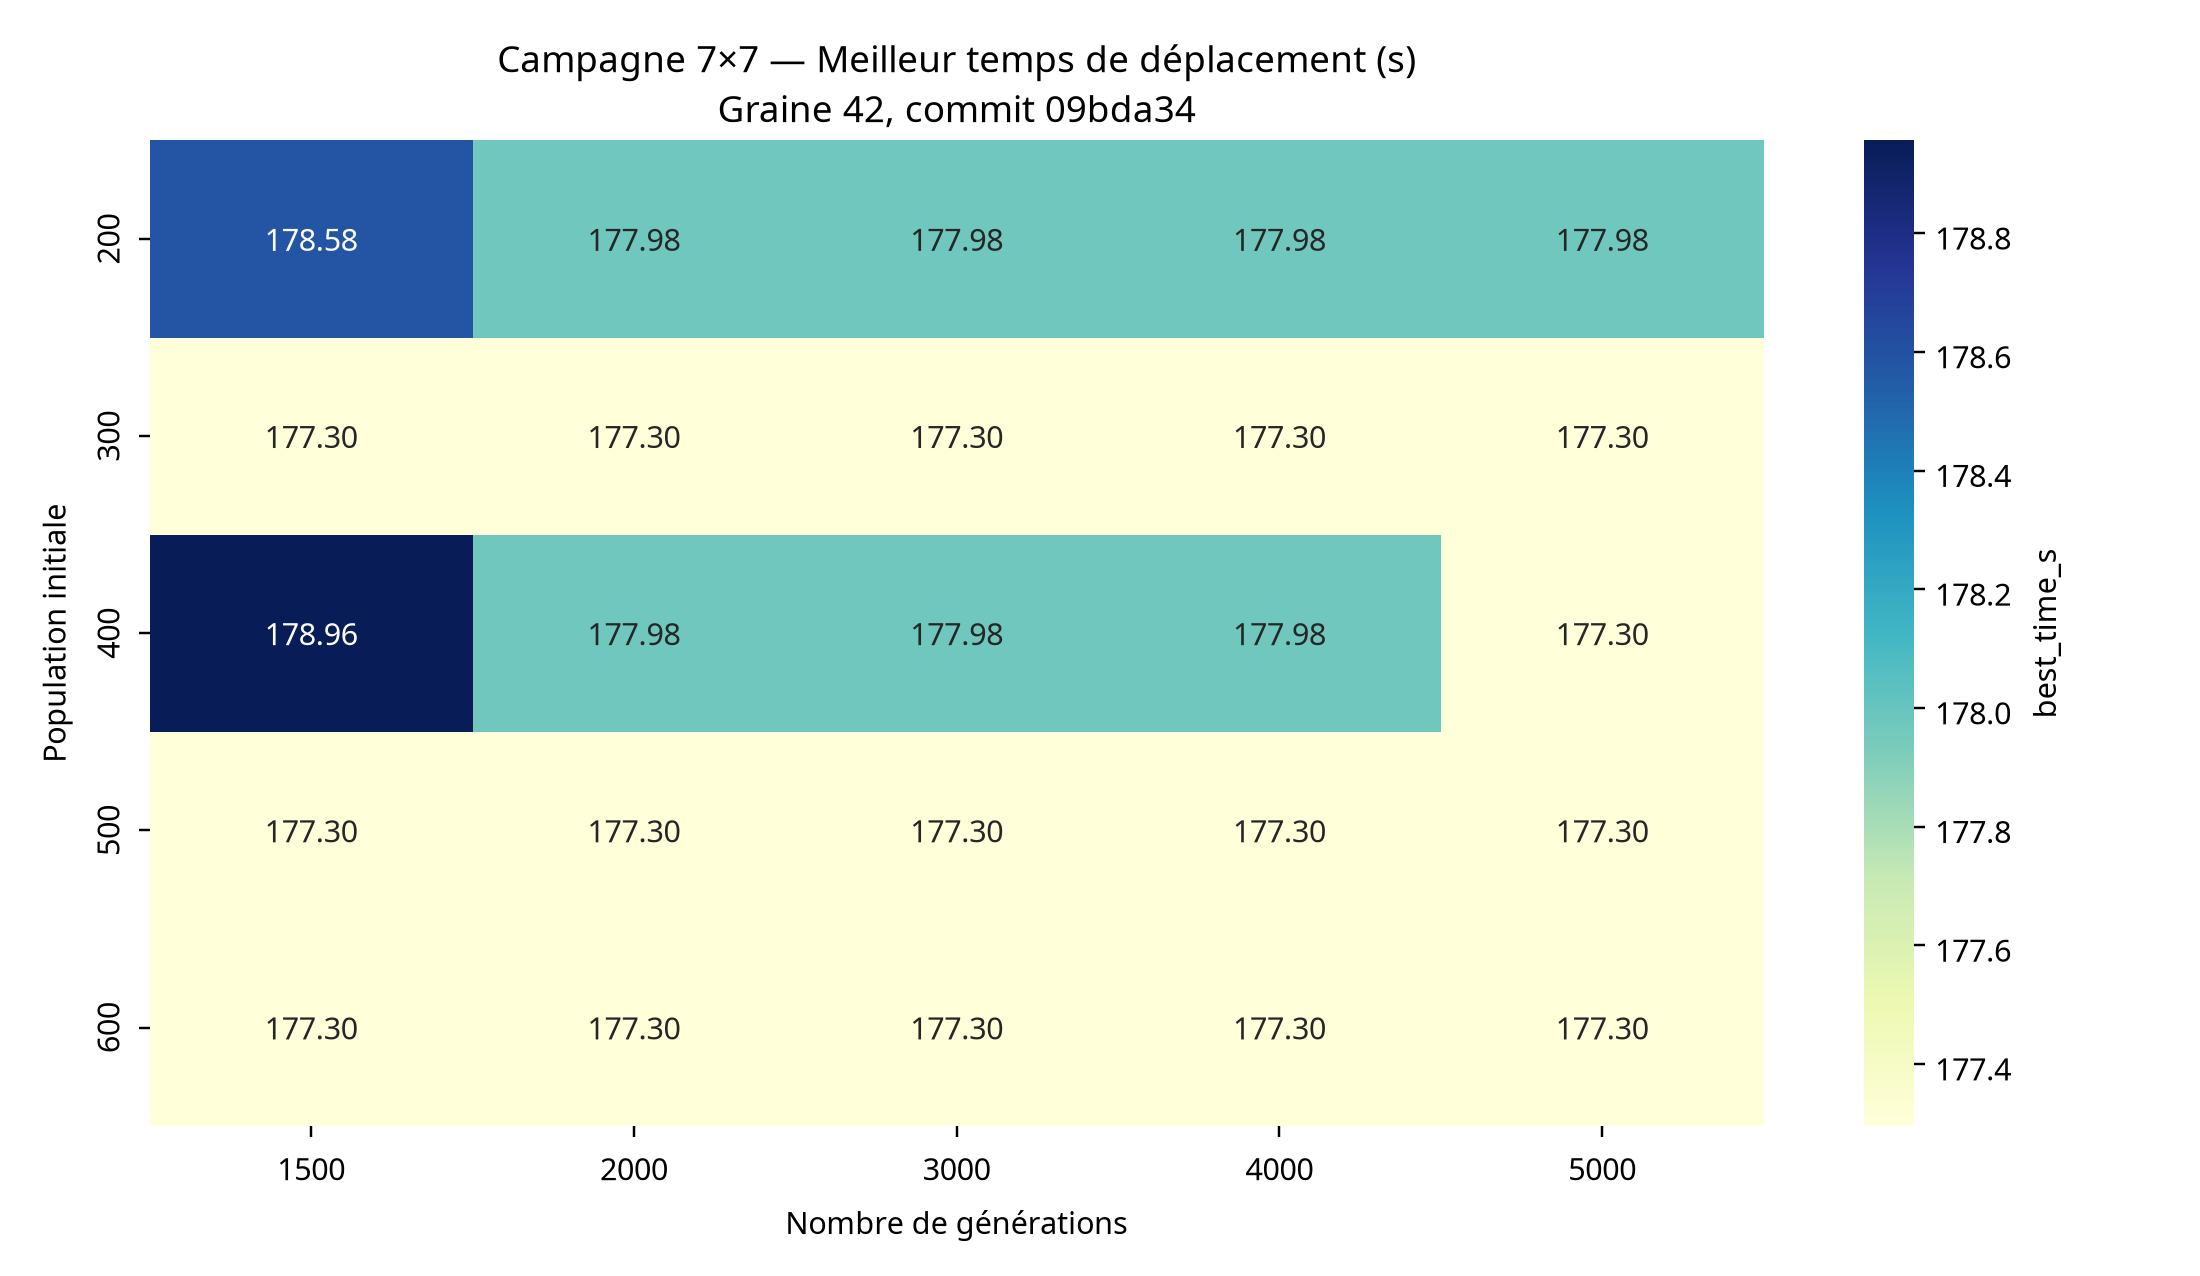
\includegraphics[width=0.92\textwidth,height=0.34\textheight,keepaspectratio]{hm_time_7x7.png}\\[0.3em]
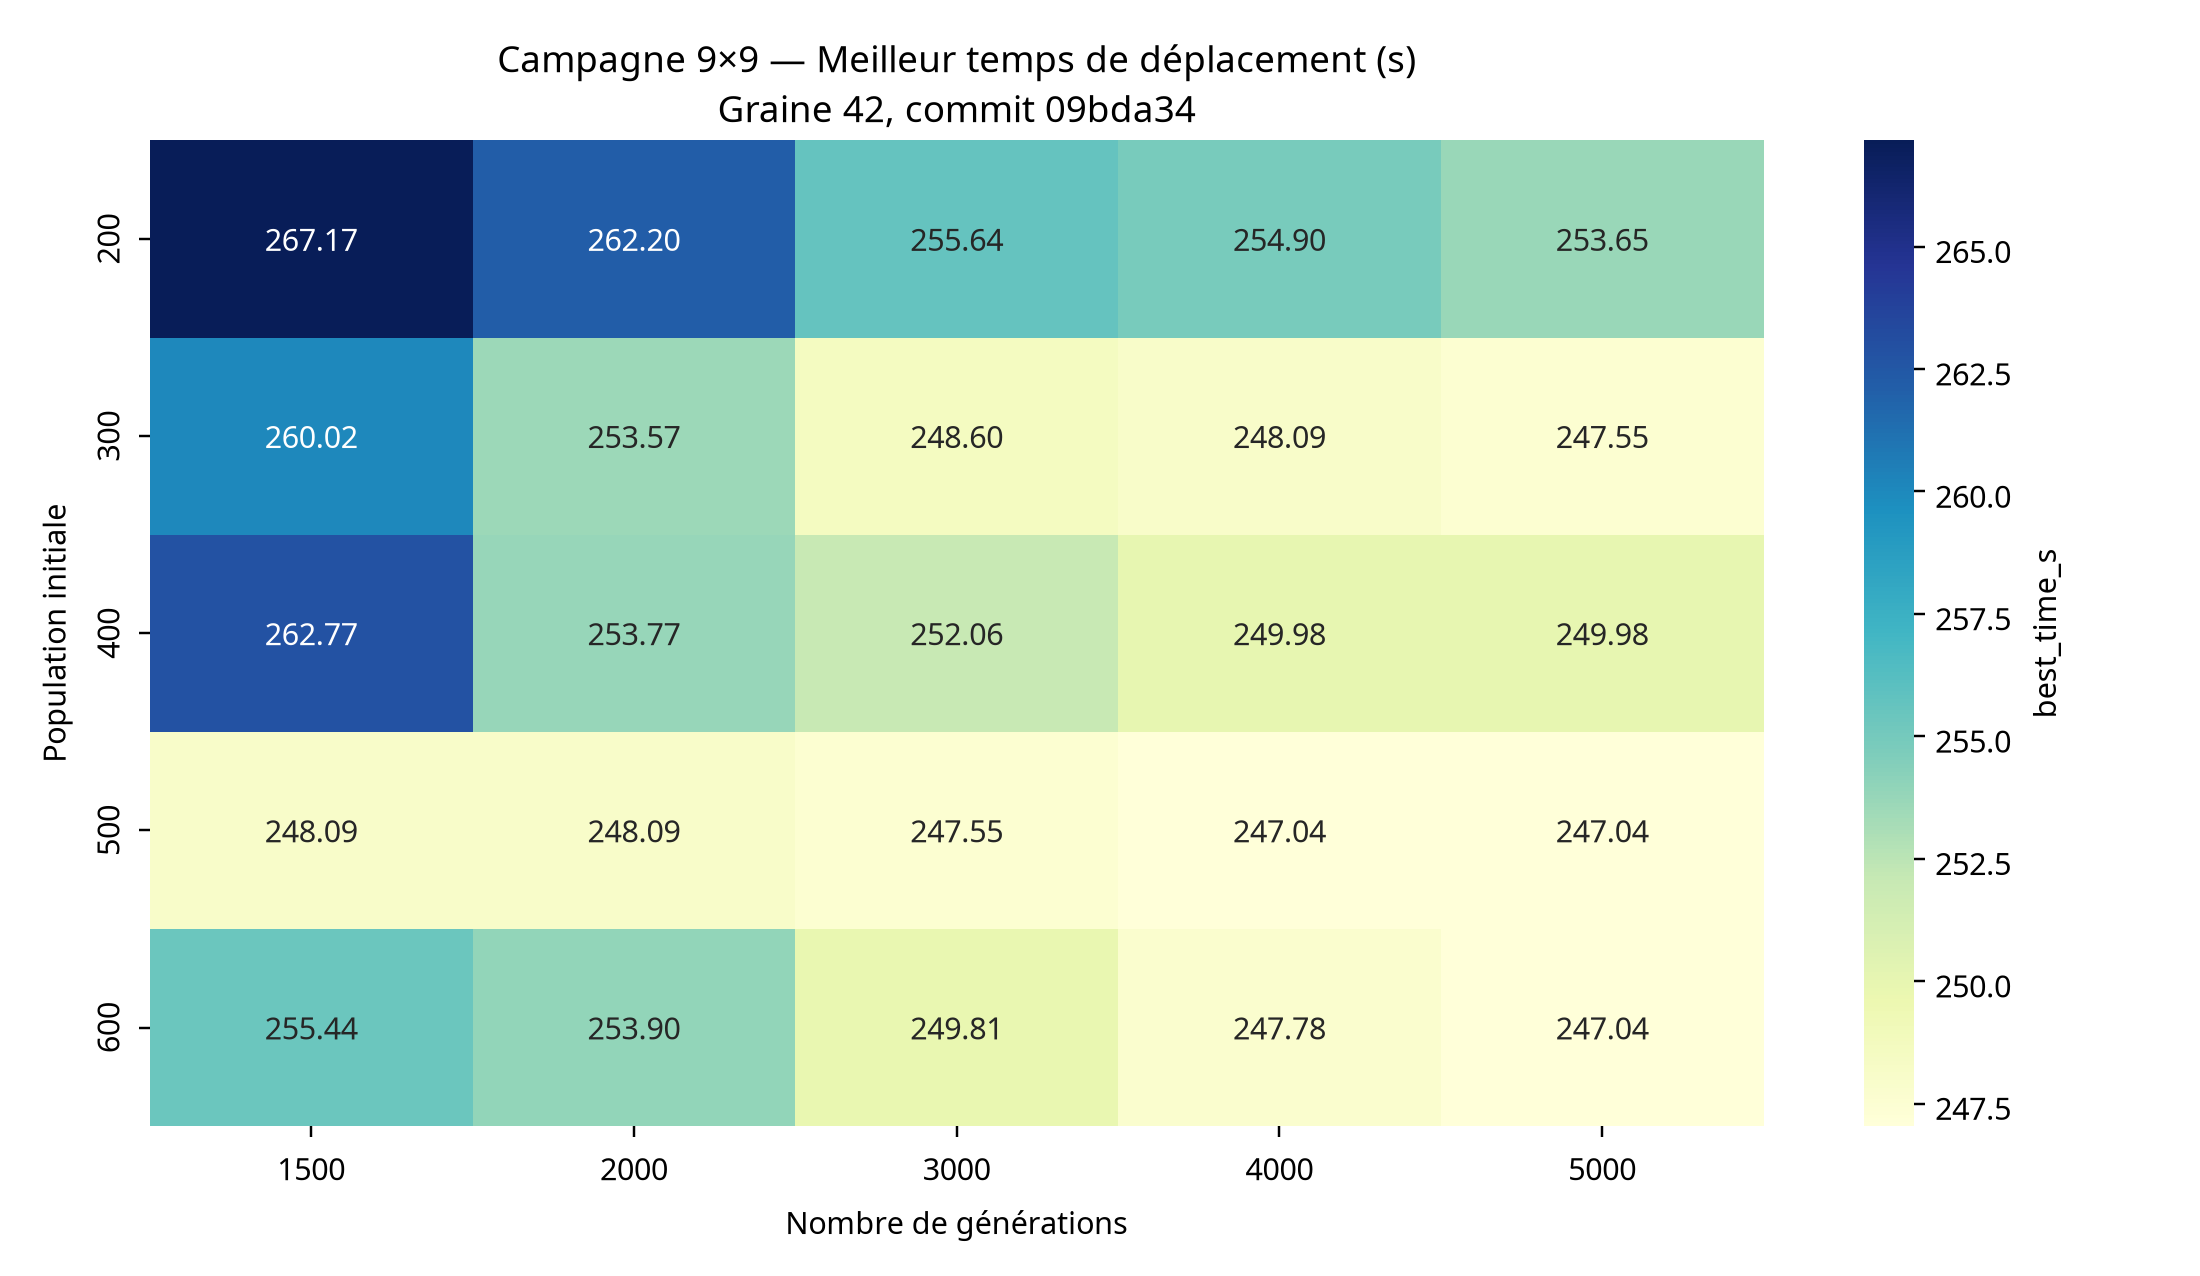
\includegraphics[width=0.92\textwidth,height=0.34\textheight,keepaspectratio]{hm_time_9x9.png}
\caption{Cartes de chaleur du meilleur temps : (a) grille $7\times7$, (b) grille $9\times9$}
\label{fig:hm_time}
\end{figure}

La convergence du temps de déplacement dépend fortement de la taille de la grille. Alors que le plateau optimal est atteint dès 1500 générations pour la grille $7\times7$, il faut attendre 5000 générations pour stabiliser la grille $9\times9$. Cela justifie le dimensionnement différencié des paramètres de NSGA-II retenu pour chaque configuration.


\begin{figure}[H]
\centering
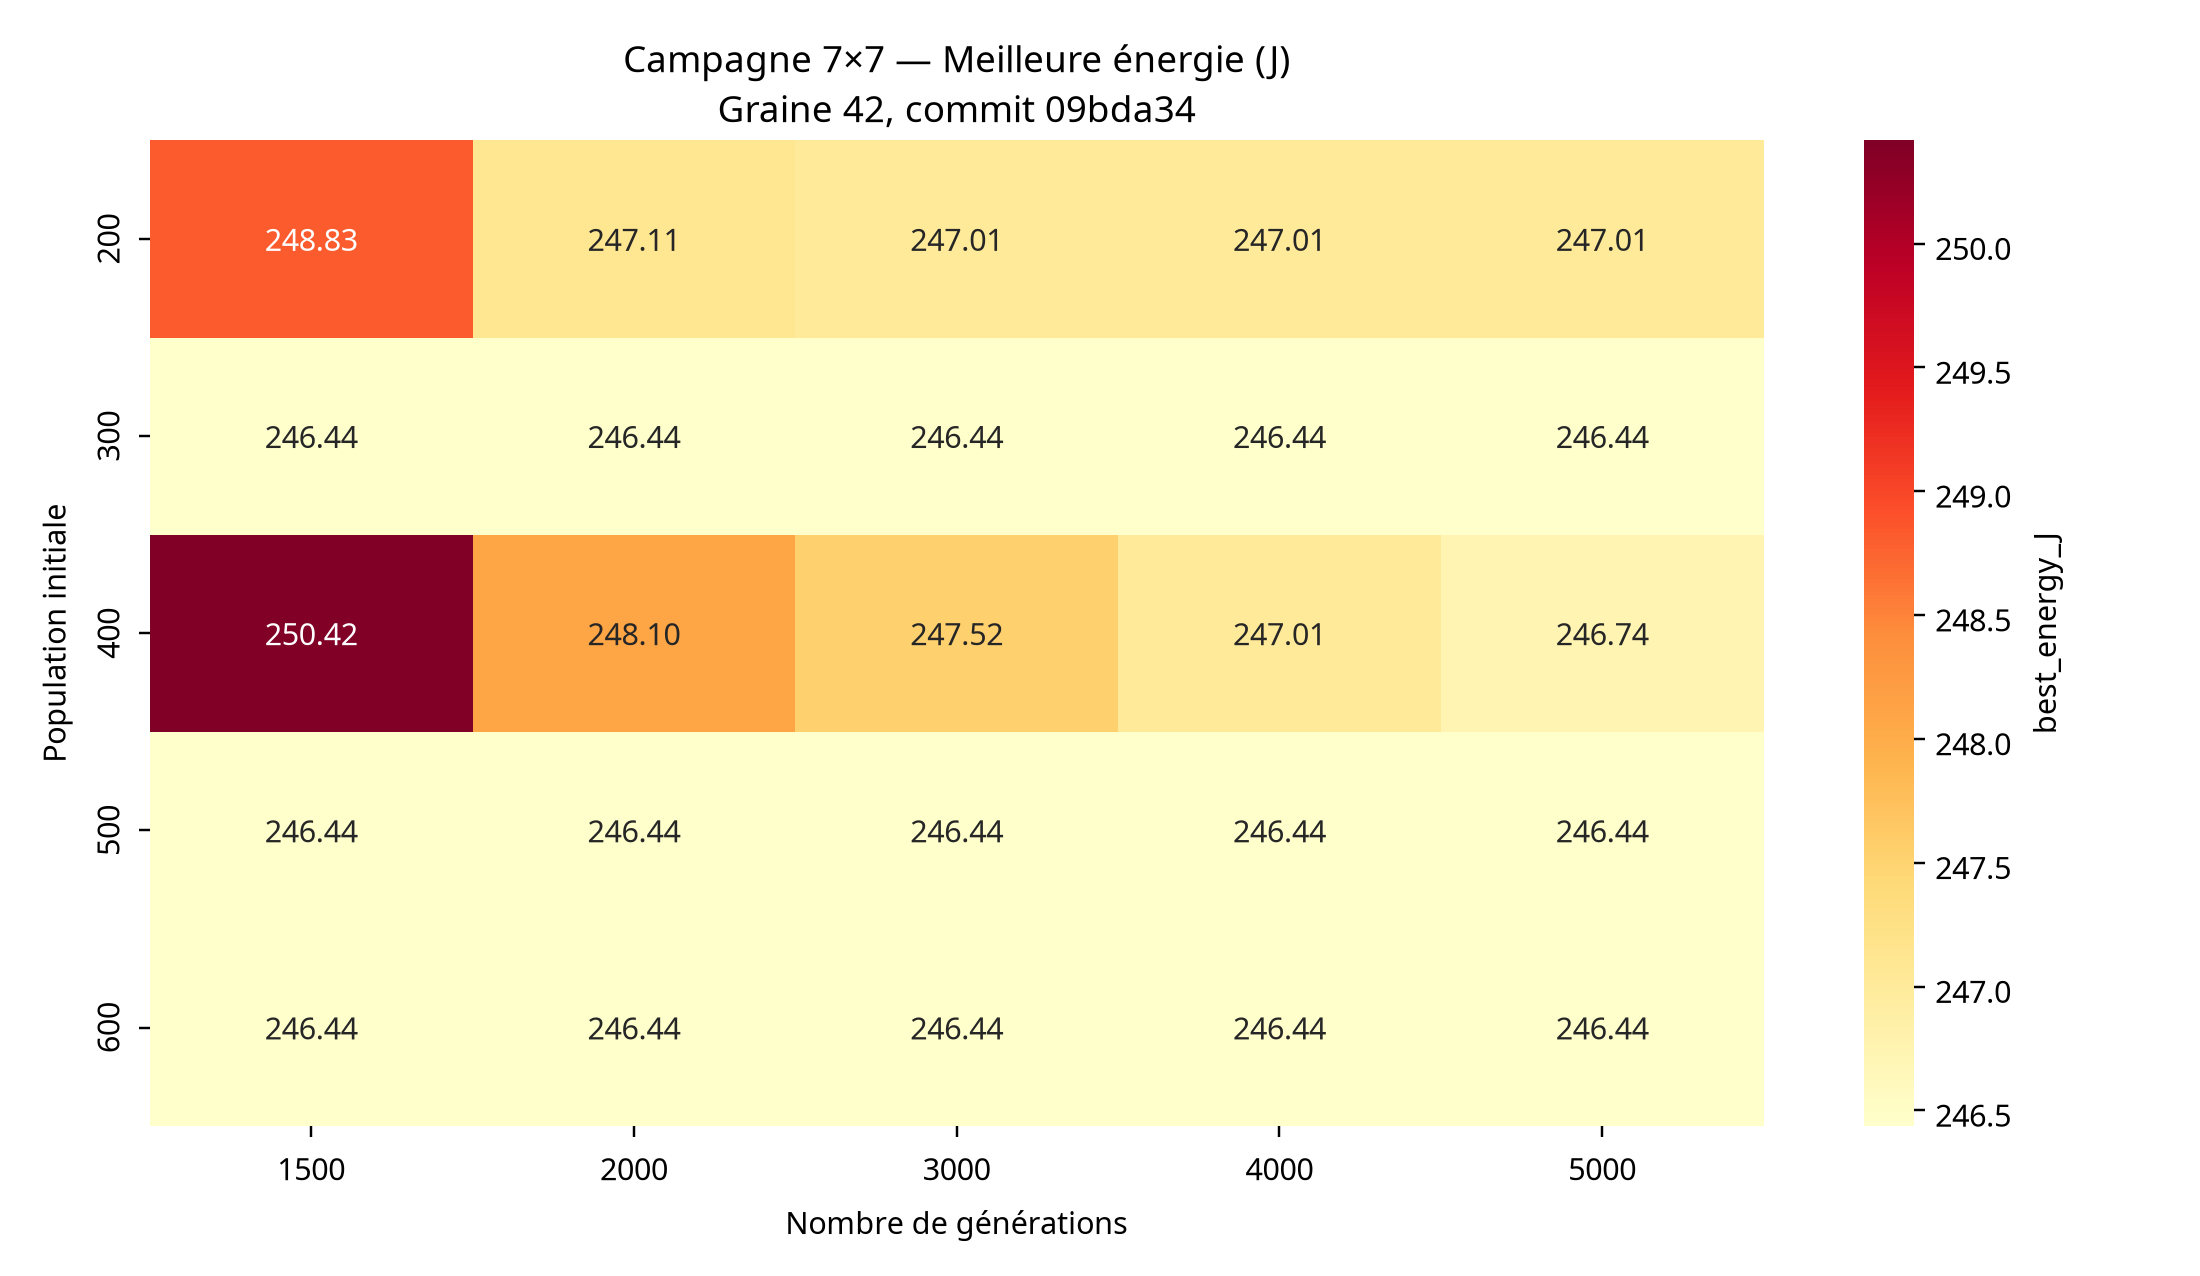
\includegraphics[width=0.92\textwidth,height=0.34\textheight,keepaspectratio]{hm_energy_7x7.png}\\[0.3em]
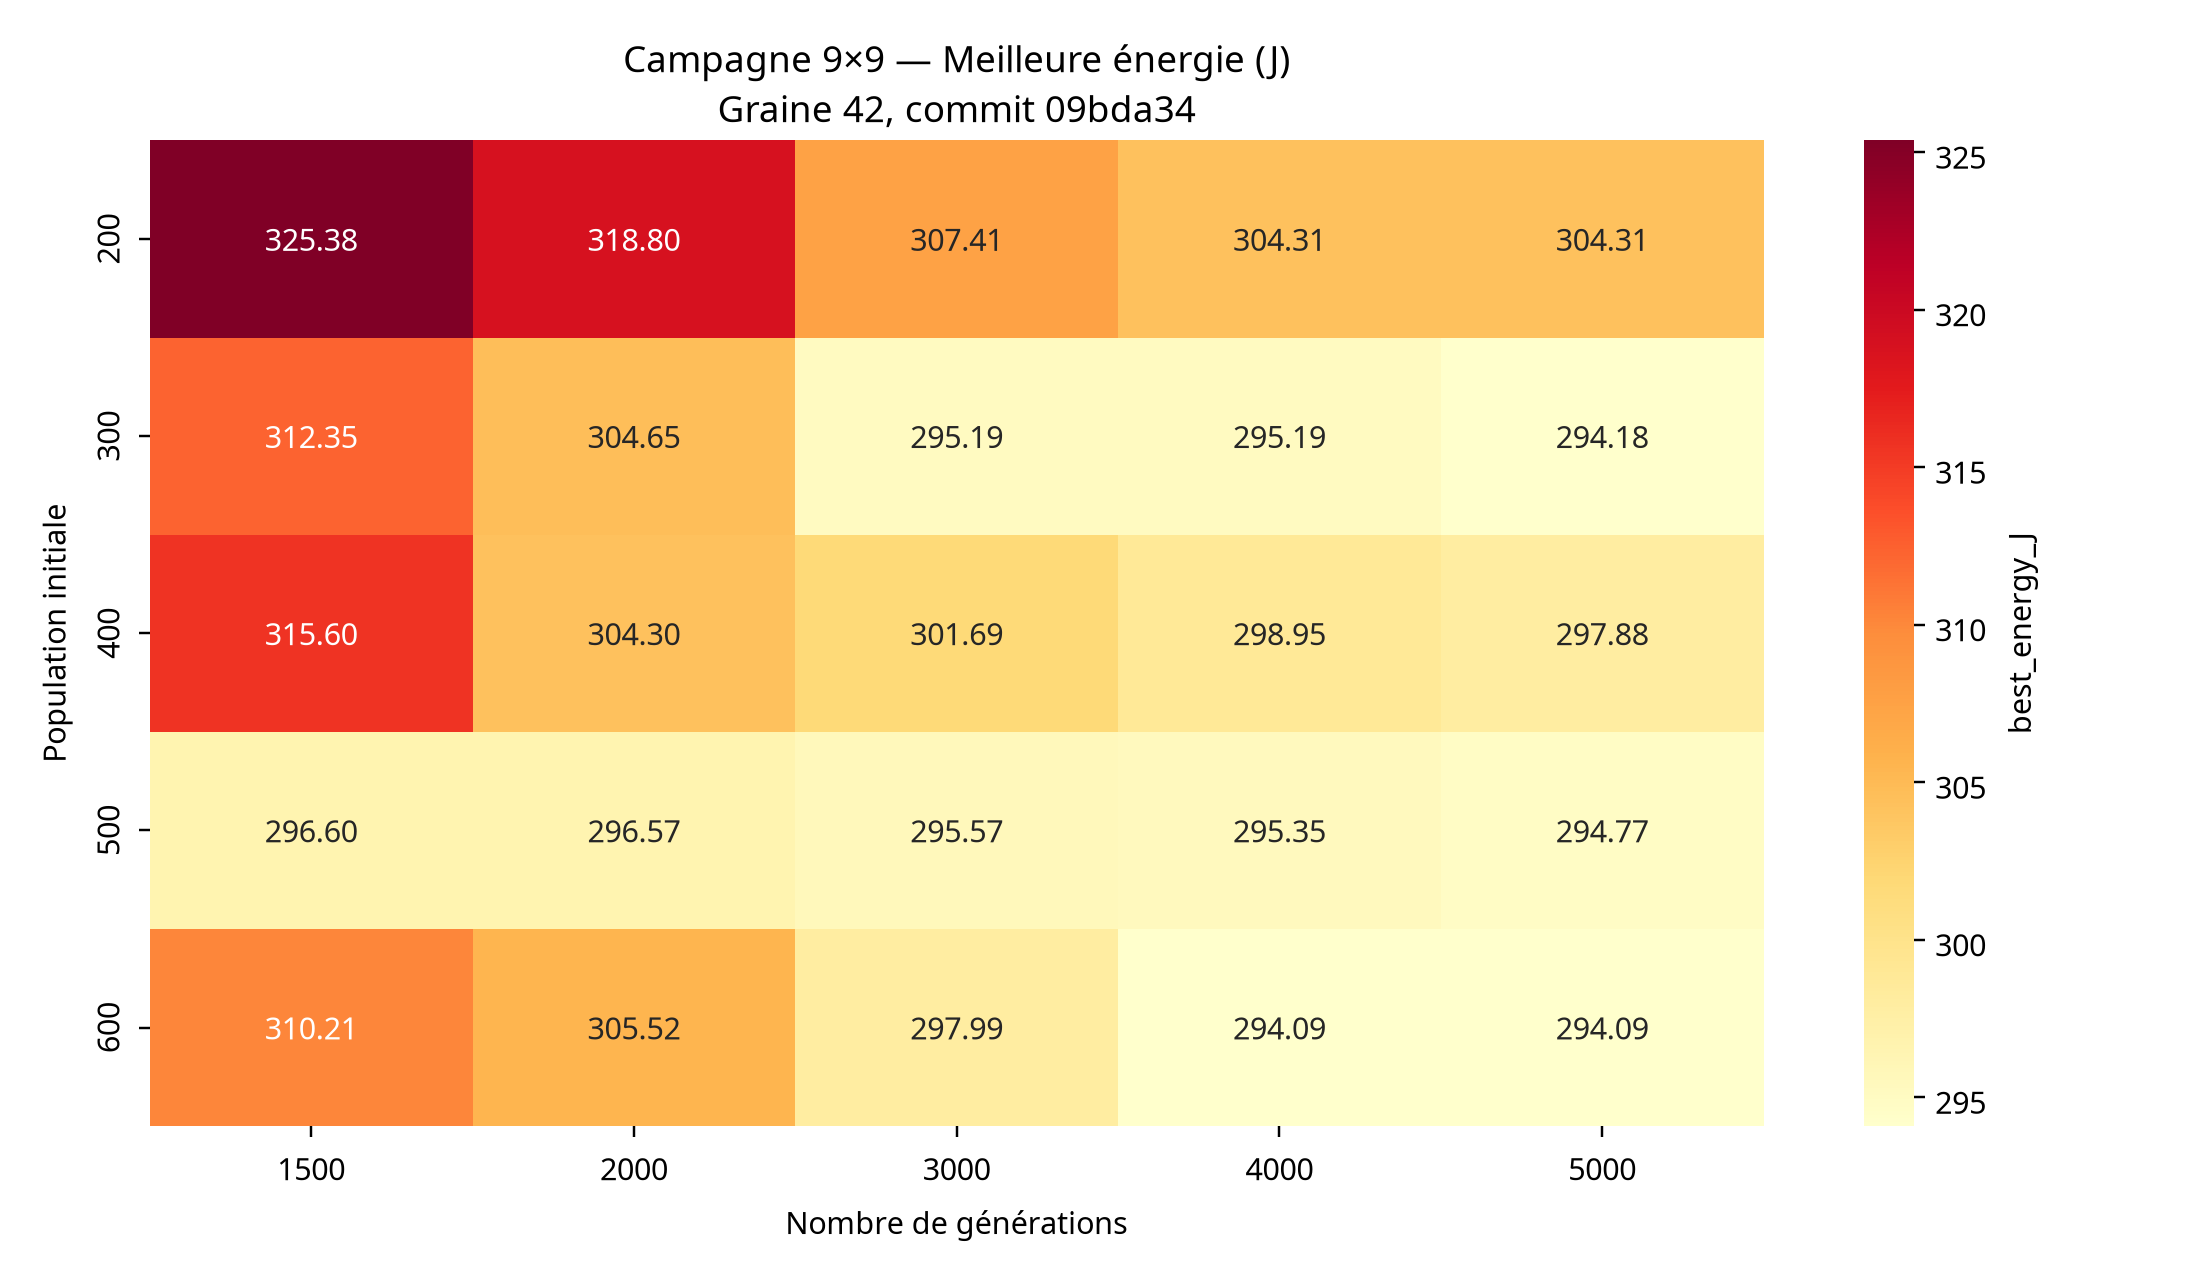
\includegraphics[width=0.92\textwidth,height=0.34\textheight,keepaspectratio]{hm_energy_9x9.png}
\caption{Cartes de chaleur de la meilleure énergie : (a) grille $7\times7$, (b) grille $9\times9$}
\label{fig:hm_energy}
\end{figure}



\begin{table}[H]
\centering
\caption{Robustesse sur trois graines (42, 30 et 100)}
\label{tab:robust}
\footnotesize
\begin{tabular}{|c|c|c|c|c|}
\hline
\textbf{Grille} & \textbf{Pop. $\times$ gén.} & \textbf{Temps $\pm\sigma$ (s)} & \textbf{Énergie $\pm\sigma$ (J)} & \textbf{Durée (s)} \\
\hline
$7\times7$ & $300\times1500$ & $178{,}31\pm0{,}89$ & $248{,}5\pm2{,}1$ & 37 \\
\hline
$7\times7$ & $500\times2000$ & $177{,}98\pm0{,}69$ & $247{,}4\pm1{,}1$ & 73 \\
\hline
$7\times7$ & $600\times3000$ & $177{,}52\pm0{,}39$ & $246{,}6\pm0{,}3$ & 132 \\
\hline
$9\times9$ & $500\times5000$ & $248{,}65\pm2{,}79$ & $295{,}9\pm3{,}2$ & 205 \\
\hline
$9\times9$ & $600\times4000$ & $247{,}44\pm0{,}39$ & $293{,}5\pm1{,}2$ & 211 \\
\hline
$9\times9$ & $600\times5000$ & $247{,}02\pm0{,}51$ & $293{,}3\pm1{,}2$ & 248 \\
\hline
\end{tabular}
\end{table}

\begin{figure}[H]
\centering
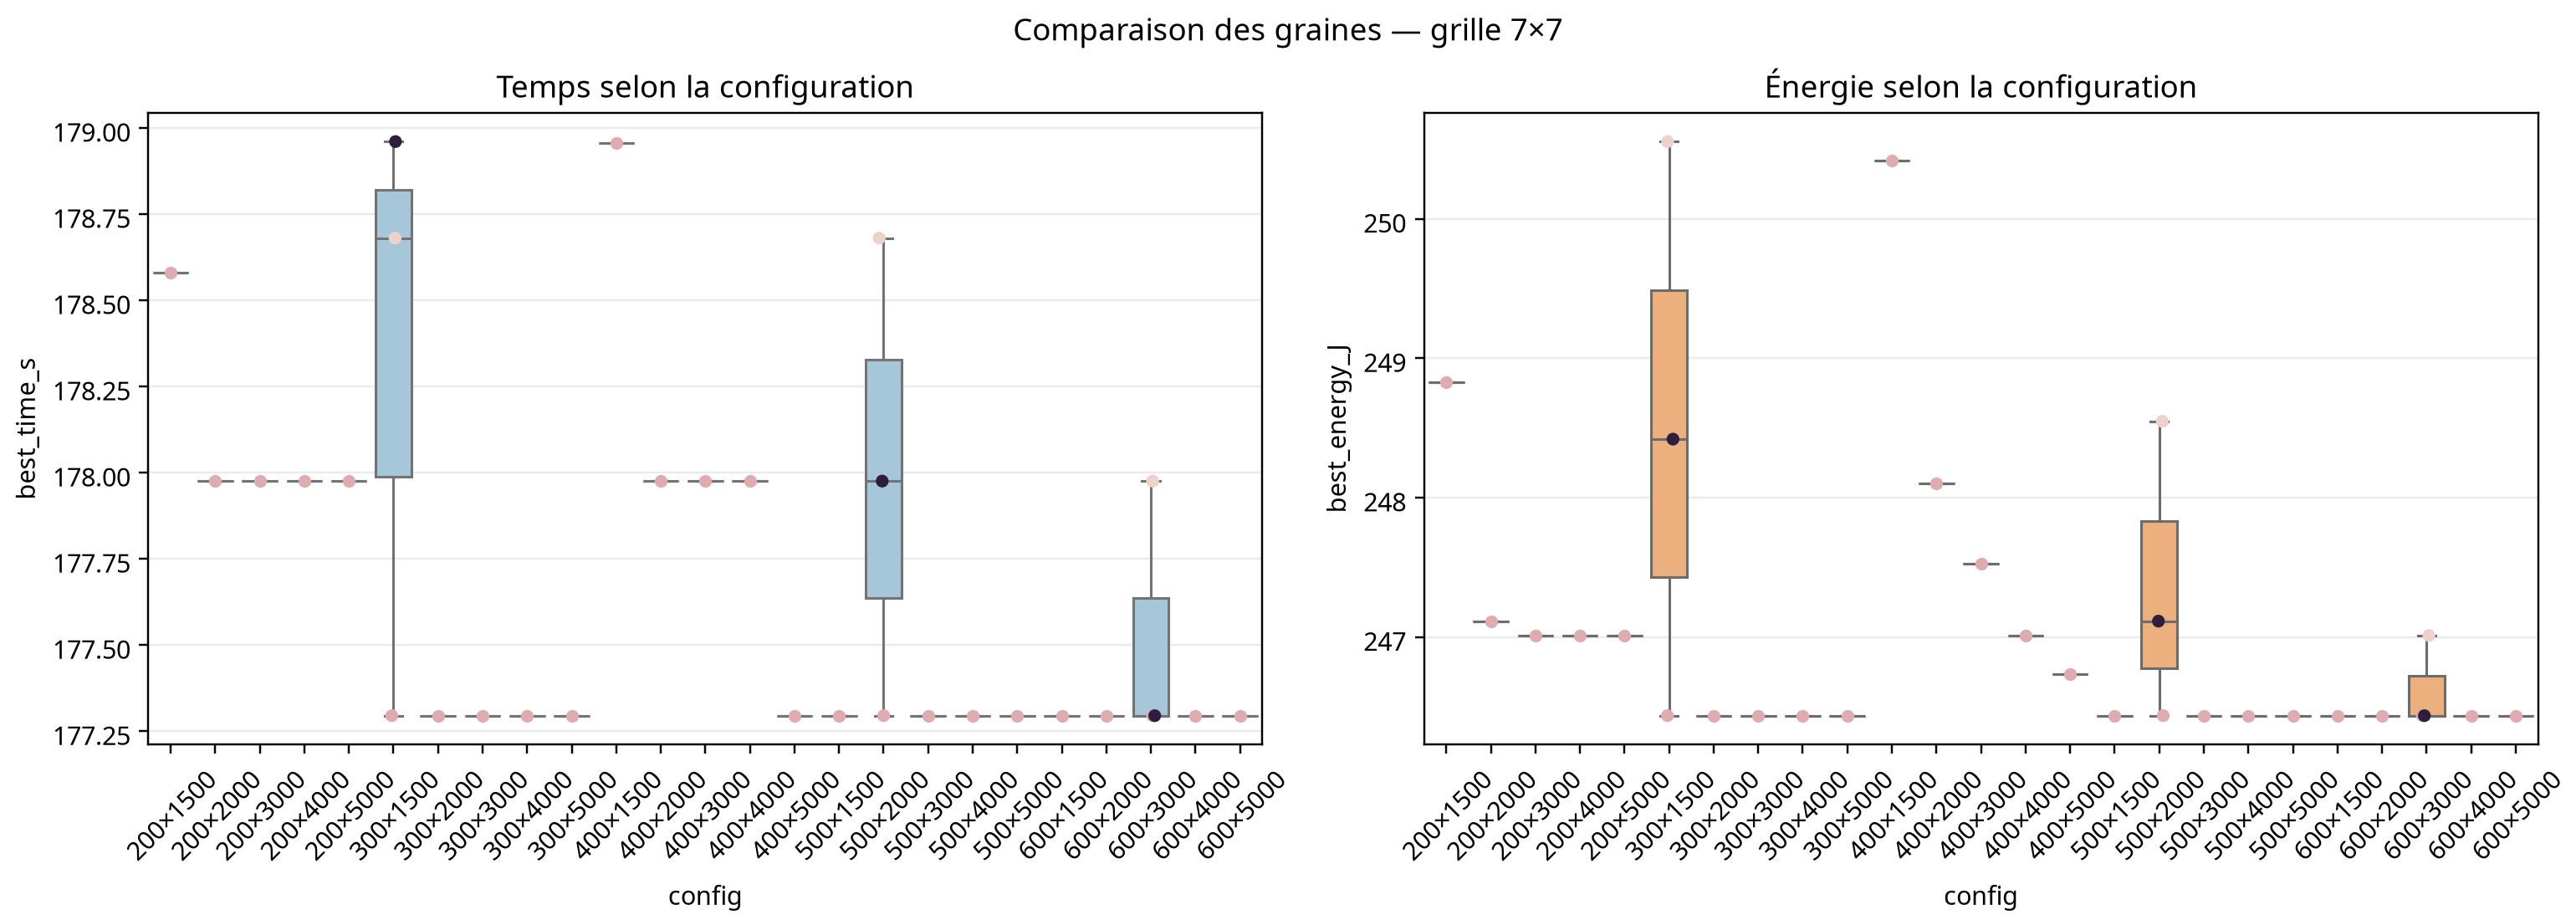
\includegraphics[width=0.92\textwidth,height=0.28\textheight,keepaspectratio]{robust_box_7x7.png}
\caption{Dispersion du temps et de l'énergie selon la configuration (grille $7\times7$)}
\label{fig:robust_box}
\end{figure}

L'analyse de la dispersion sur 50 exécutions révèle une réduction drastique de la variabilité (boîtes plus courtes, disparition des valeurs aberrantes) lorsque la taille de la population augmente. Une population de 500 individus garantit ainsi une stabilité et une reproductibilité accrues de l'algorithme, indépendamment du hasard.


\begin{figure}[H]
\centering
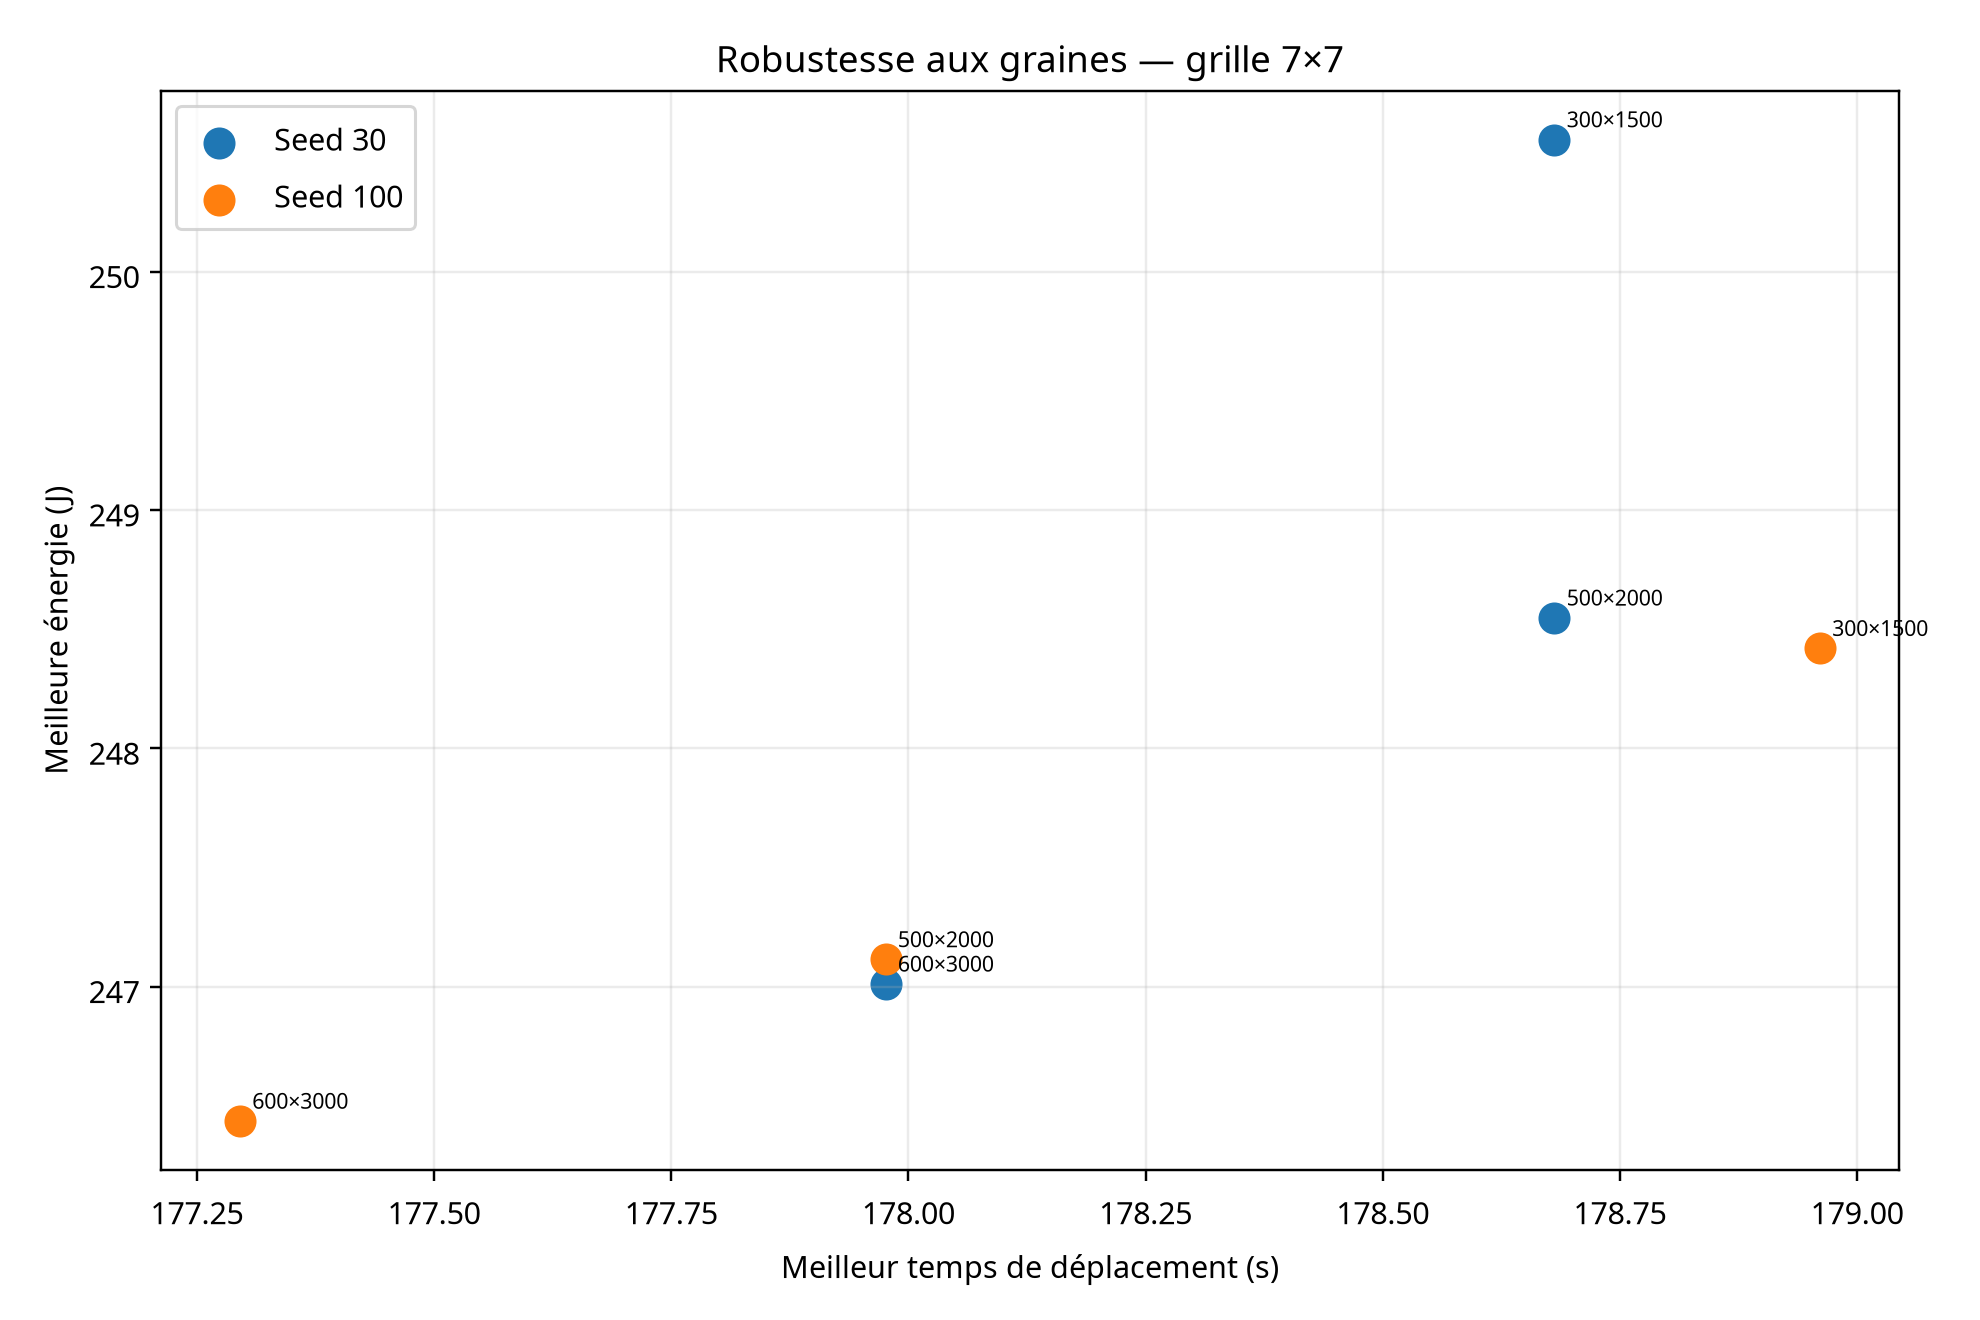
\includegraphics[width=0.90\textwidth,height=0.26\textheight,keepaspectratio]{robust_seeds_7x7.png}\\[0.2em]
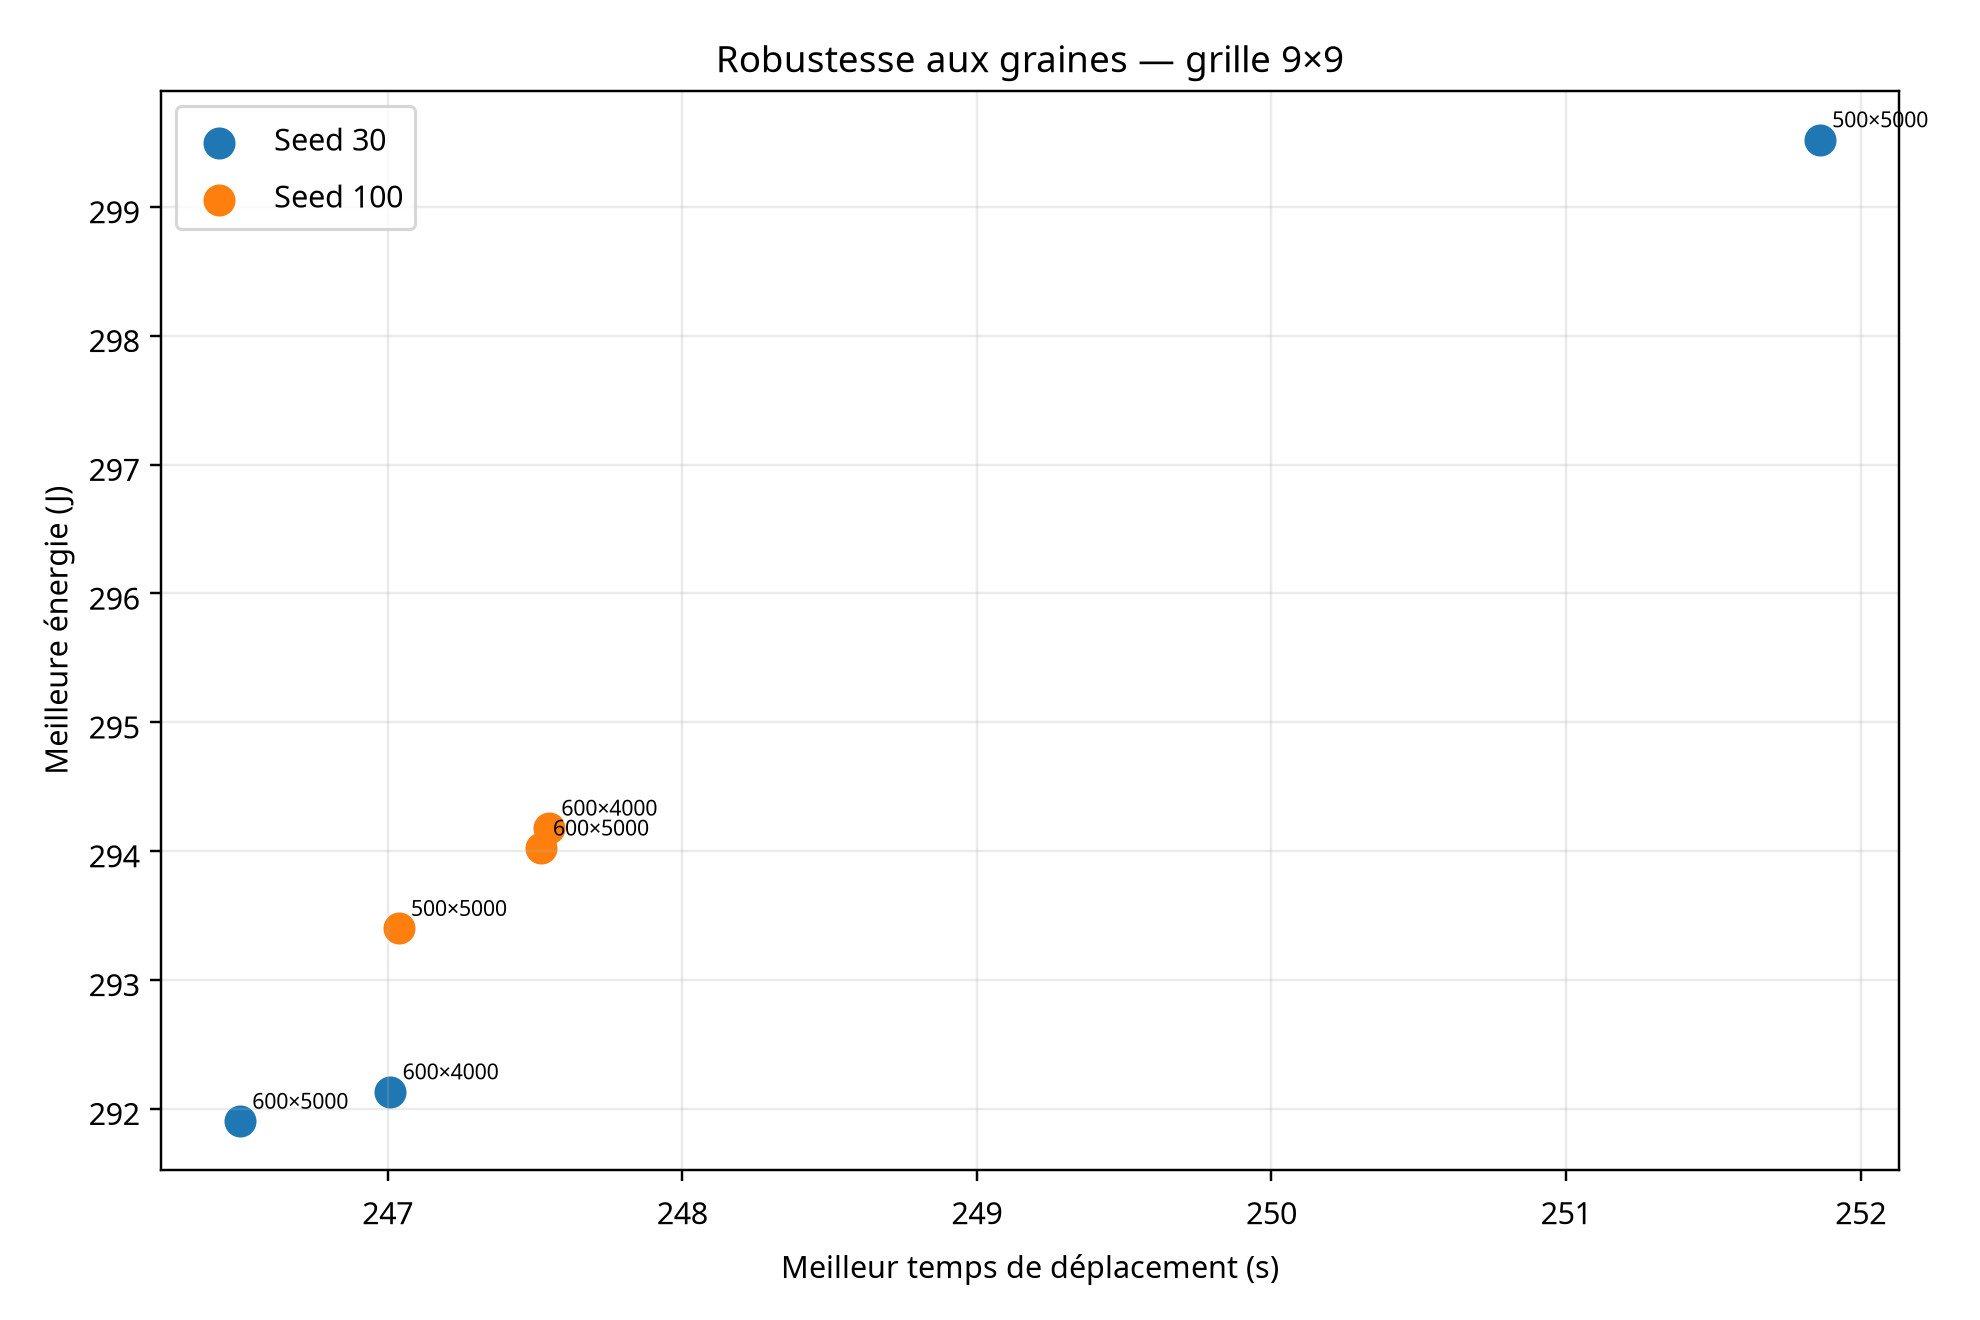
\includegraphics[width=0.90\textwidth,height=0.26\textheight,keepaspectratio]{robust_seeds_9x9.png}
\caption{Positions des graines 30 et 100 dans le plan temps--énergie}
\label{fig:robust_seeds}
\end{figure}

La comparaison des graines aléatoires (30 et 100) montre un regroupement spatial très serré des solutions dans l'espace des objectifs. Cette convergence démontre la robustesse statistique de NSGA-II : la qualité de la trajectoire optimisée ne dépend pas d'un «~coup de chance~», mais converge systématiquement vers les meilleures performances.


\begin{table}[H]
\centering
\caption{Paramètres retenus}
\label{tab:params}
\begin{tabular}{|c|c|c|p{7cm}|}
\hline
\textbf{Grille} & \textbf{Population} & \textbf{Générations} & \textbf{Justification} \\
\hline
$7\times7$ & 500 & 2000 & Meilleur résultat graine 42 en 73~s, dispersion modérée \\
\hline
$9\times9$ & 600 & 5000 & Meilleure moyenne (247,02~s ; 293,3~J), dispersion faible \\
\hline
\end{tabular}
\end{table}

\section{Vérification numérique}
\label{sec:verif}

\begin{table}[H]
\centering
\caption{Résultats de validation du run de référence $7\times7$}
\label{tab:valid}
\footnotesize
\begin{tabular}{|p{5cm}|c|p{7cm}|}
\hline
\textbf{Invariant} & \textbf{Statut} & \textbf{Évidence} \\
\hline
Cohérence de la configuration & PASS & $N=49$ ; $T\in[1;58]$~N ; orientation fixe \\
\hline
Faisabilité des points filtrés & PASS & 49 points ; aucun infaisable \\
\hline
Symétrie de la matrice de coûts & PASS & 2401 entrées ; symétrie ; diagonale nulle \\
\hline
Non-dominance (front de Pareto) & WARN & Une solution non dominée unique \\
\hline
Cohérence des trajectoires & PASS & 3 types ; centre aux extrémités \\
\hline
Profils cinématiques & PASS & 5361 échantillons ; $v_{\max}=0{,}045$~m/s \\
\hline
Cohérence croisée & PASS & Profils, matrice et résumé concordants \\
\hline
\end{tabular}
\end{table}

Résultat : 6 PASS, 1 WARN, 0 FAIL sur les 50 exécutions. Le WARN signale un front trop réduit pour étudier le compromis temps--énergie.

\section{Résultats et analyse}

\subsection{Configuration de référence (zone sécurisée)}

Pour la grille $7\times7$ : solution unique 177,30~s / 246,44~J contre baseline 229,3~s / 340,3~J (gains 22,7~\% et 27,6~\%). Pour la grille $9\times9$ : temps minimal 247,04~s, énergie minimale 294,09~J contre baseline 312,9~s / 412,6~J (gains 21,0~\% et 28,7~\%).

\begin{table}[H]
\centering
\caption{Résultats de la configuration de référence}
\label{tab:res_ref}
\footnotesize
\begin{tabular}{|c|c|c|c|c|c|c|c|}
\hline
\textbf{Grille} & \textbf{Temps (s)} & \textbf{Énergie (J)} & \textbf{Baseline} & \textbf{Gain t} & \textbf{Gain E} & \textbf{Stab.} & \textbf{Total} \\
\hline
$7\times7$ & 177,30 & 246,44 & 229,3 / 340,3 & 22,7~\% & 27,6~\% & 98~s & 275,3~s \\
\hline
$9\times9$ & 247,04 & 294,09 & 312,9 / 412,6 & 21,0~\% & 28,7~\% & 162~s & 409,0~s \\
\hline
\end{tabular}
\end{table}

\begin{figure}[H]
\centering
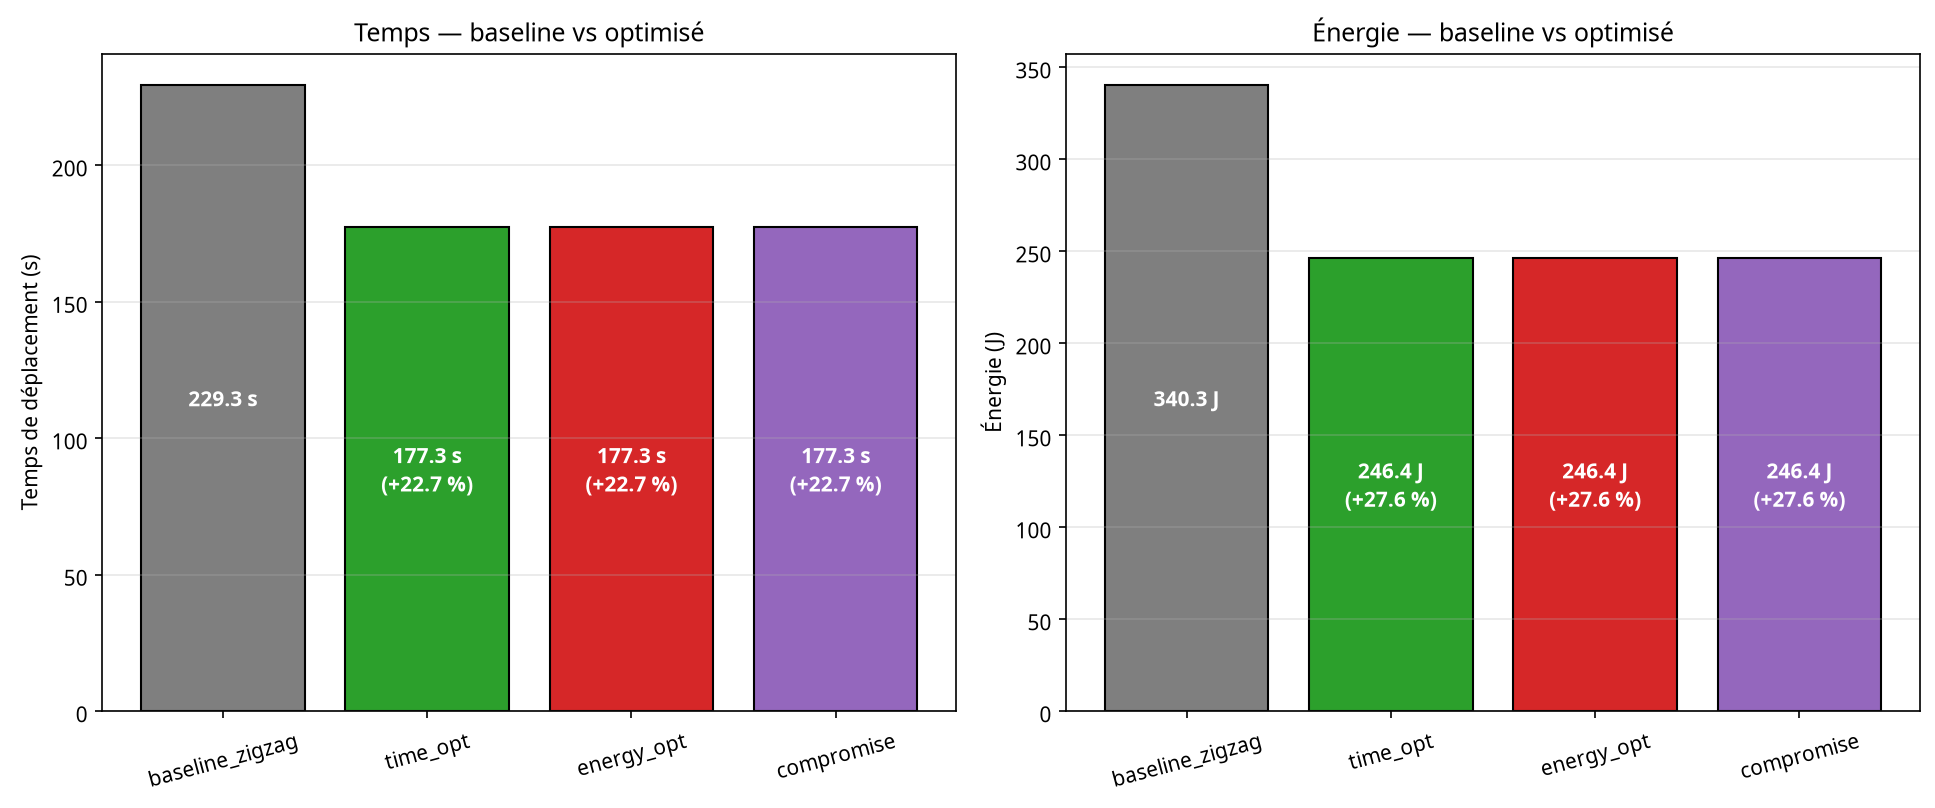
\includegraphics[width=0.92\textwidth,height=0.34\textheight,keepaspectratio]{comp_sec_7x7.png}\\[0.3em]
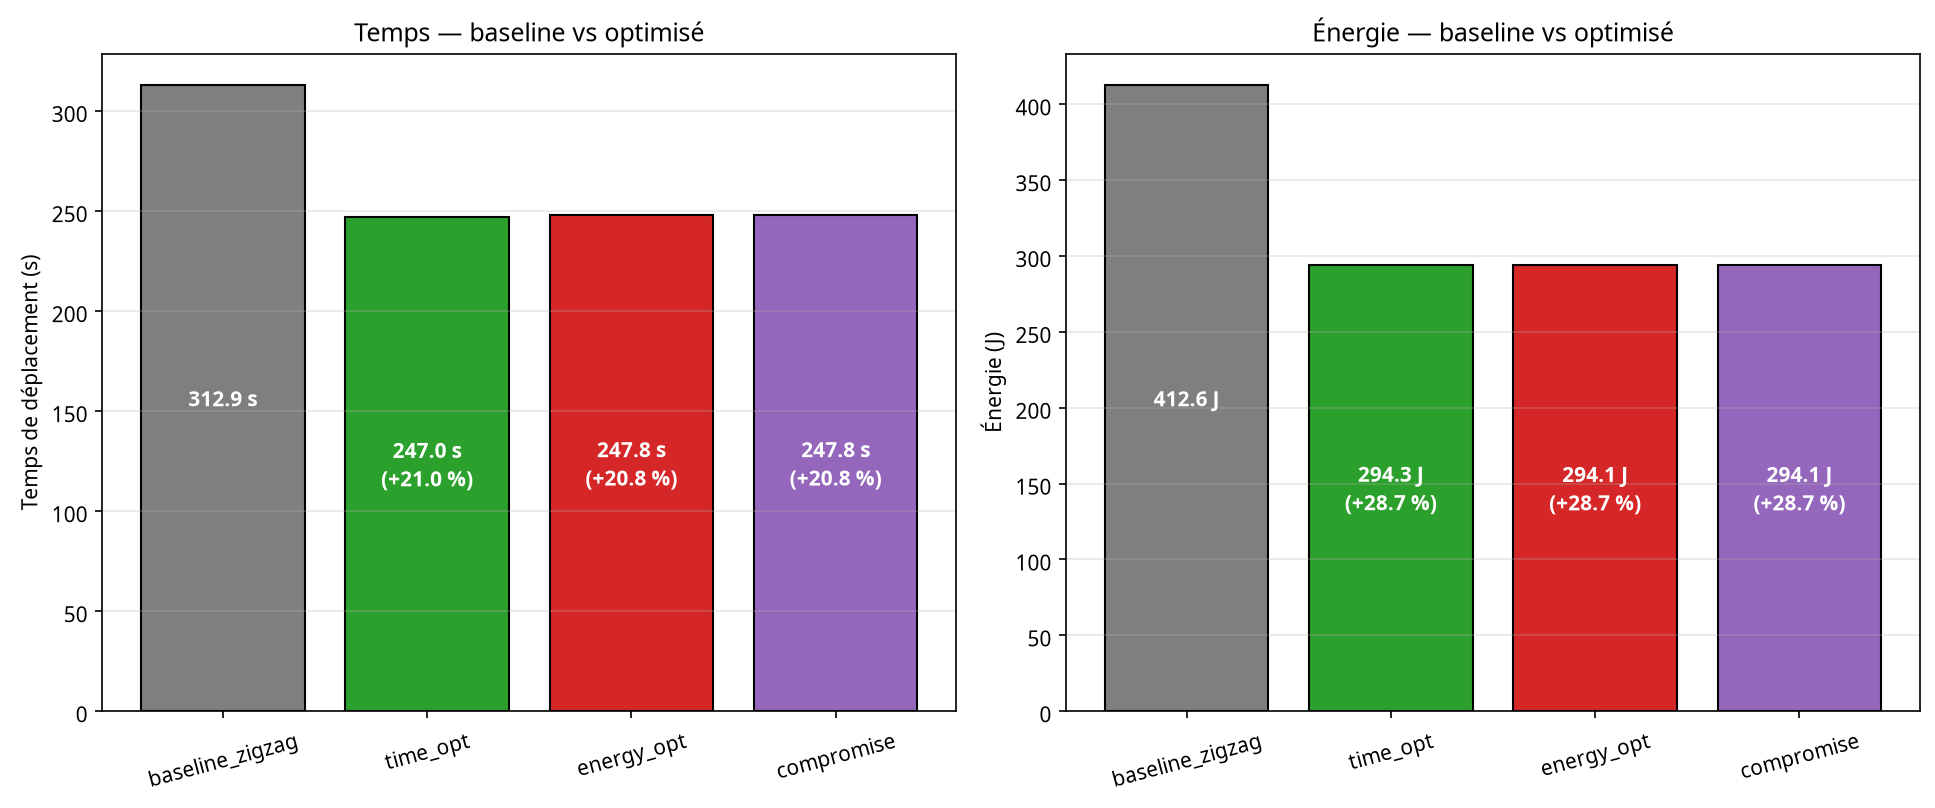
\includegraphics[width=0.92\textwidth,height=0.34\textheight,keepaspectratio]{comp_sec_9x9.png}
\caption{Temps et énergie : baseline zigzag et trajectoires optimisées, zone sécurisée}
\label{fig:comp_sec}
\end{figure}

La comparaison en barres met en évidence l'écart de performance entre le balayage en zigzag (gris) et les trajectoires optimisées (vert, rouge, violet) sur les deux tailles de grille. Le point clé est la réduction systématique et visible de la hauteur des barres colorées par rapport à la référence, illustrant les gains substantiels obtenus. Pour la grille $7\times7$, les trois solutions optimisées se superposent parfaitement (solution unique), tandis que pour la grille $9\times9$, elles présentent des variations minimes. Cette visualisation valide quantitativement l'efficacité de l'algorithme NSGA-II, qui permet de réduire le temps de mouvement de 21,0~\% à 22,7~\% et l'énergie mécanique de 27,6~\% à 28,7~\% par rapport à une approche conventionnelle.


\begin{figure}[H]
\centering
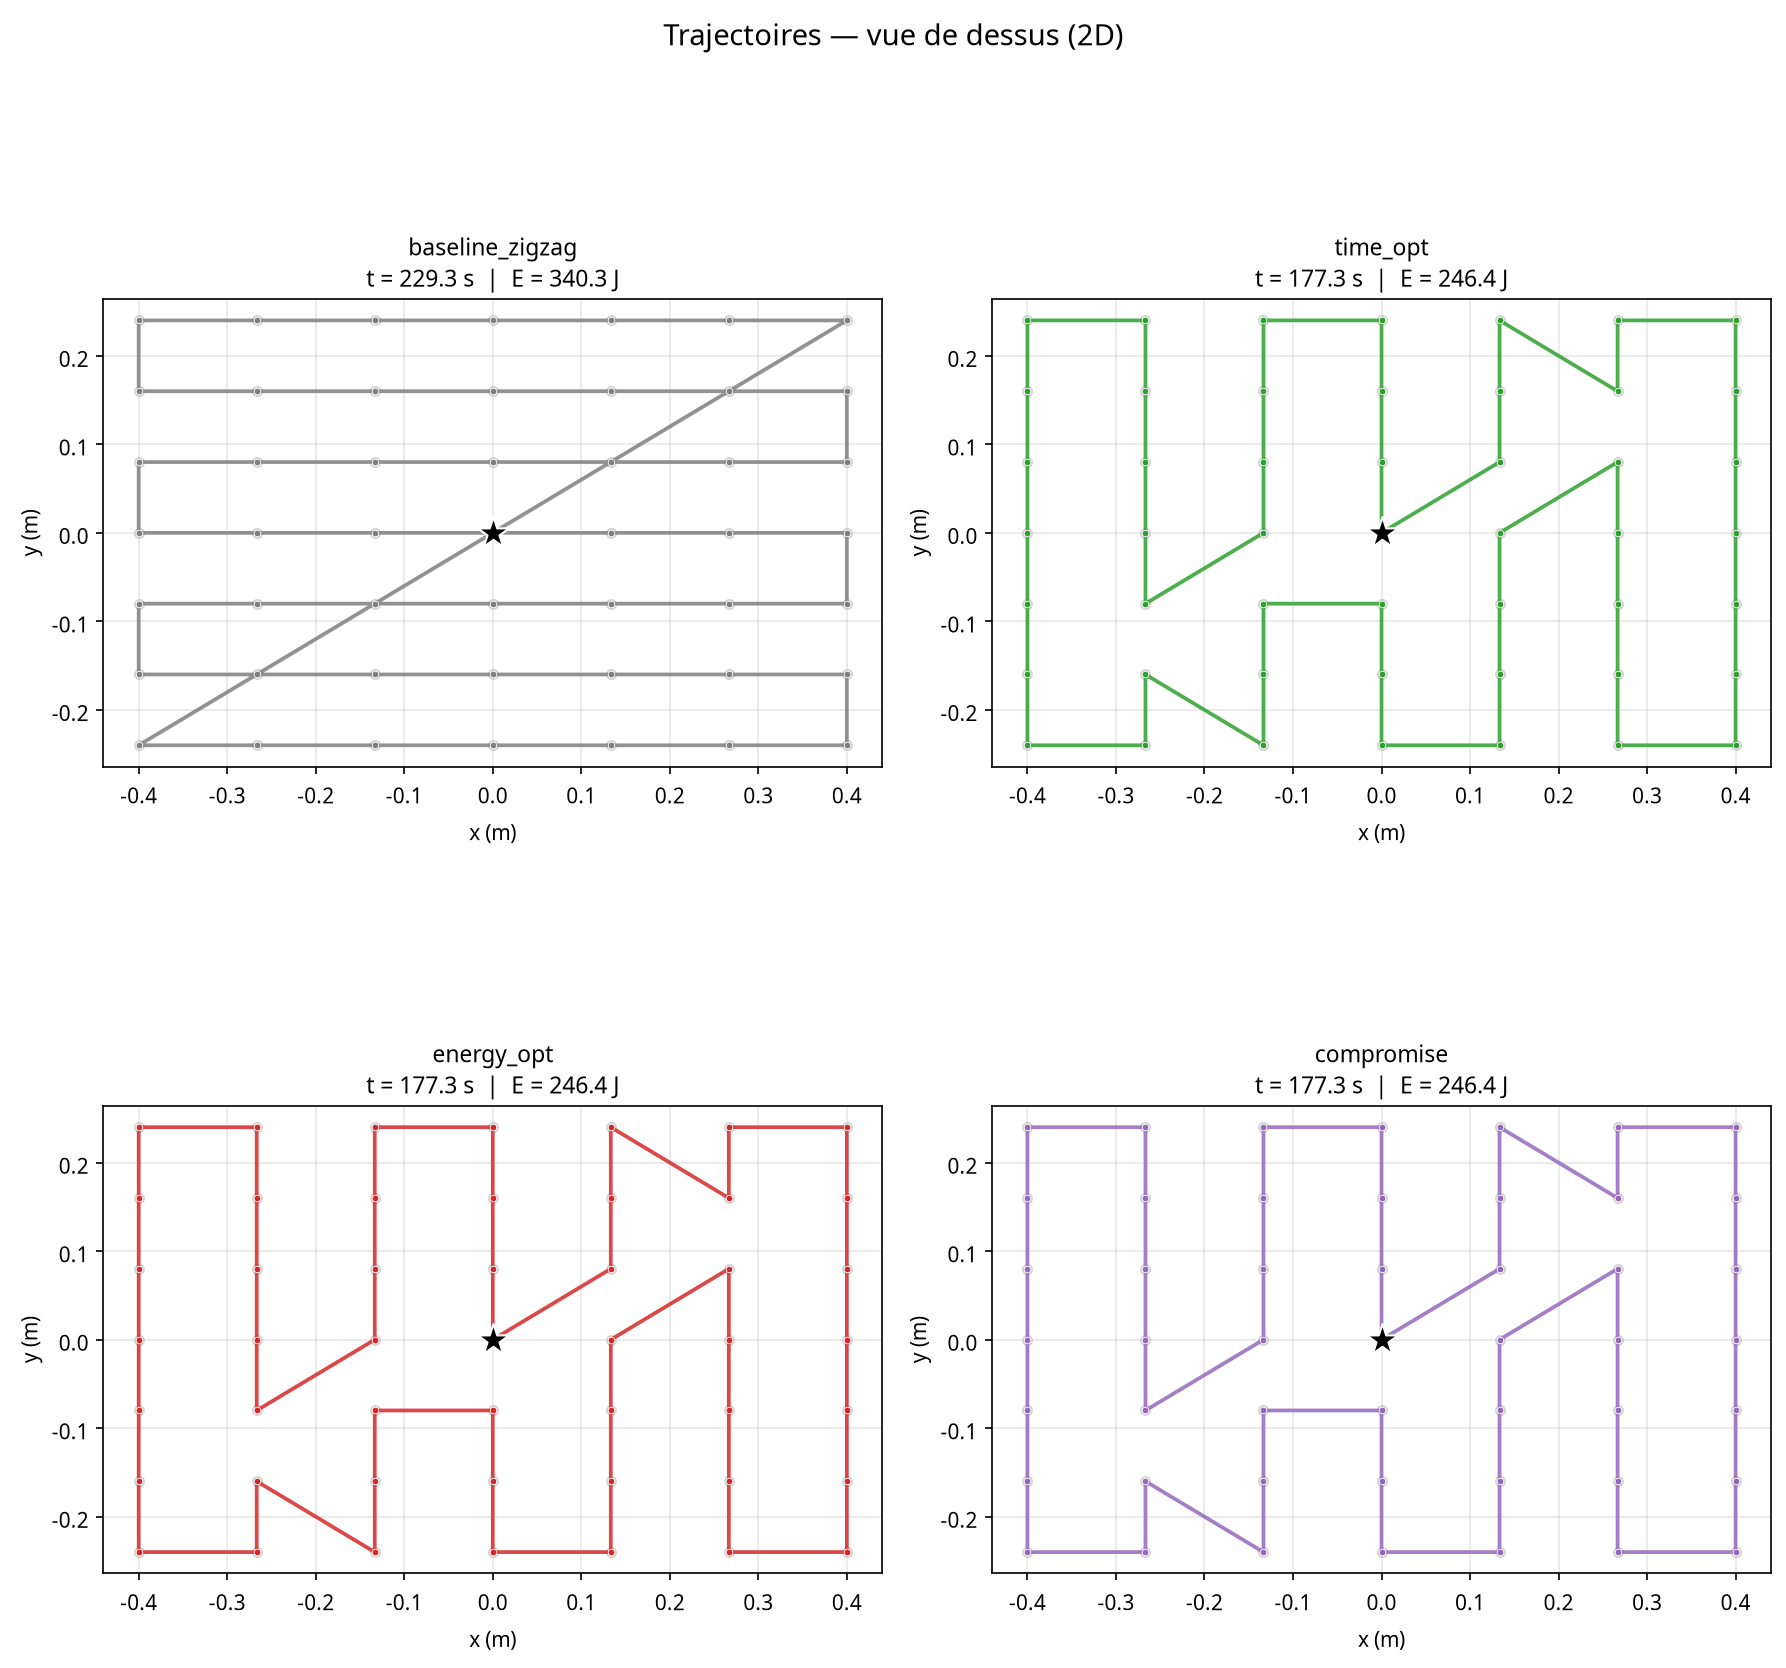
\includegraphics[width=\textwidth]{traj_sec_7x7.png}
\caption{Trajectoire en zone sécurisée pour grille $7\times7$}
\label{fig:traj_sec_7}
\end{figure}

La comparaison visuelle met en évidence la rupture entre la baseline en zigzag (gris) et les trajectoires optimisées. Le point clé est la superposition parfaite des trois courbes (vert, rouge, violet) : elles empruntent exactement le même chemin, confirmant visuellement que le front de Pareto se réduit à une solution unique (singleton) pour cette configuration. Contrairement au balayage systématique ligne par ligne, l'algorithme trace un parcours fluide qui évite les croisements et les retours inutiles, validant ainsi les gains de 22,7~\% en temps et de 27,6~\% en énergie observés sur la grille $7\times7$.

\clearpage
\begin{figure}[H]
\centering
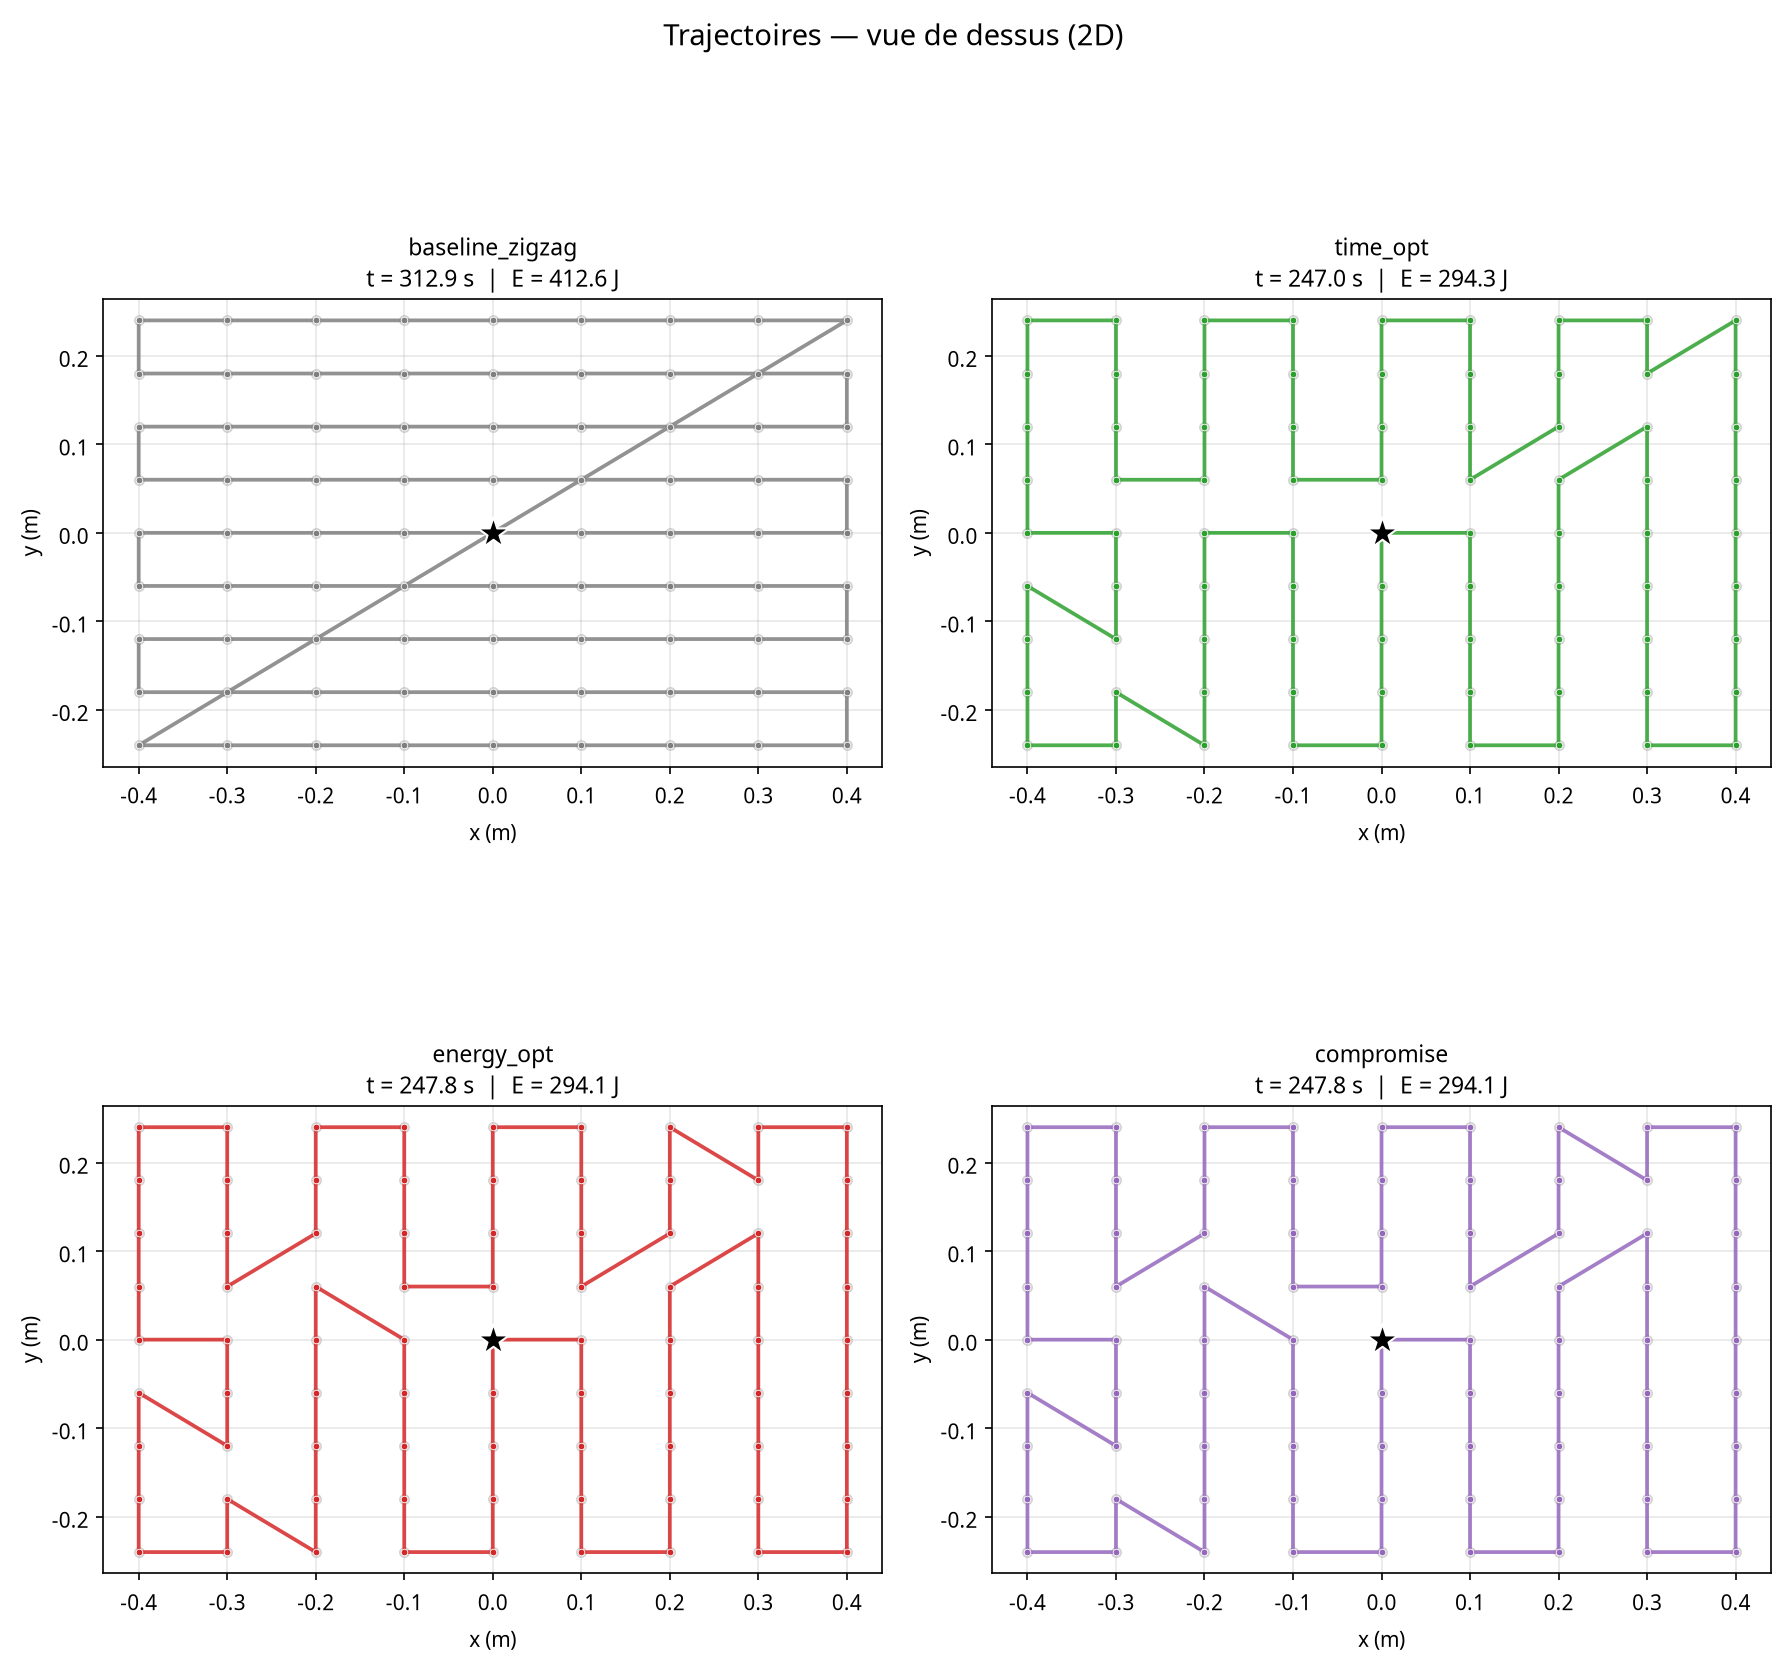
\includegraphics[width=\textwidth]{traj_sec_9x9.png}
\caption{Trajectoire en zone sécurisée pour grille $9\times9$}
\label{fig:traj_sec_9}
\end{figure}

\begin{figure}[H]
\centering
\begin{minipage}{0.48\textwidth}
\centering
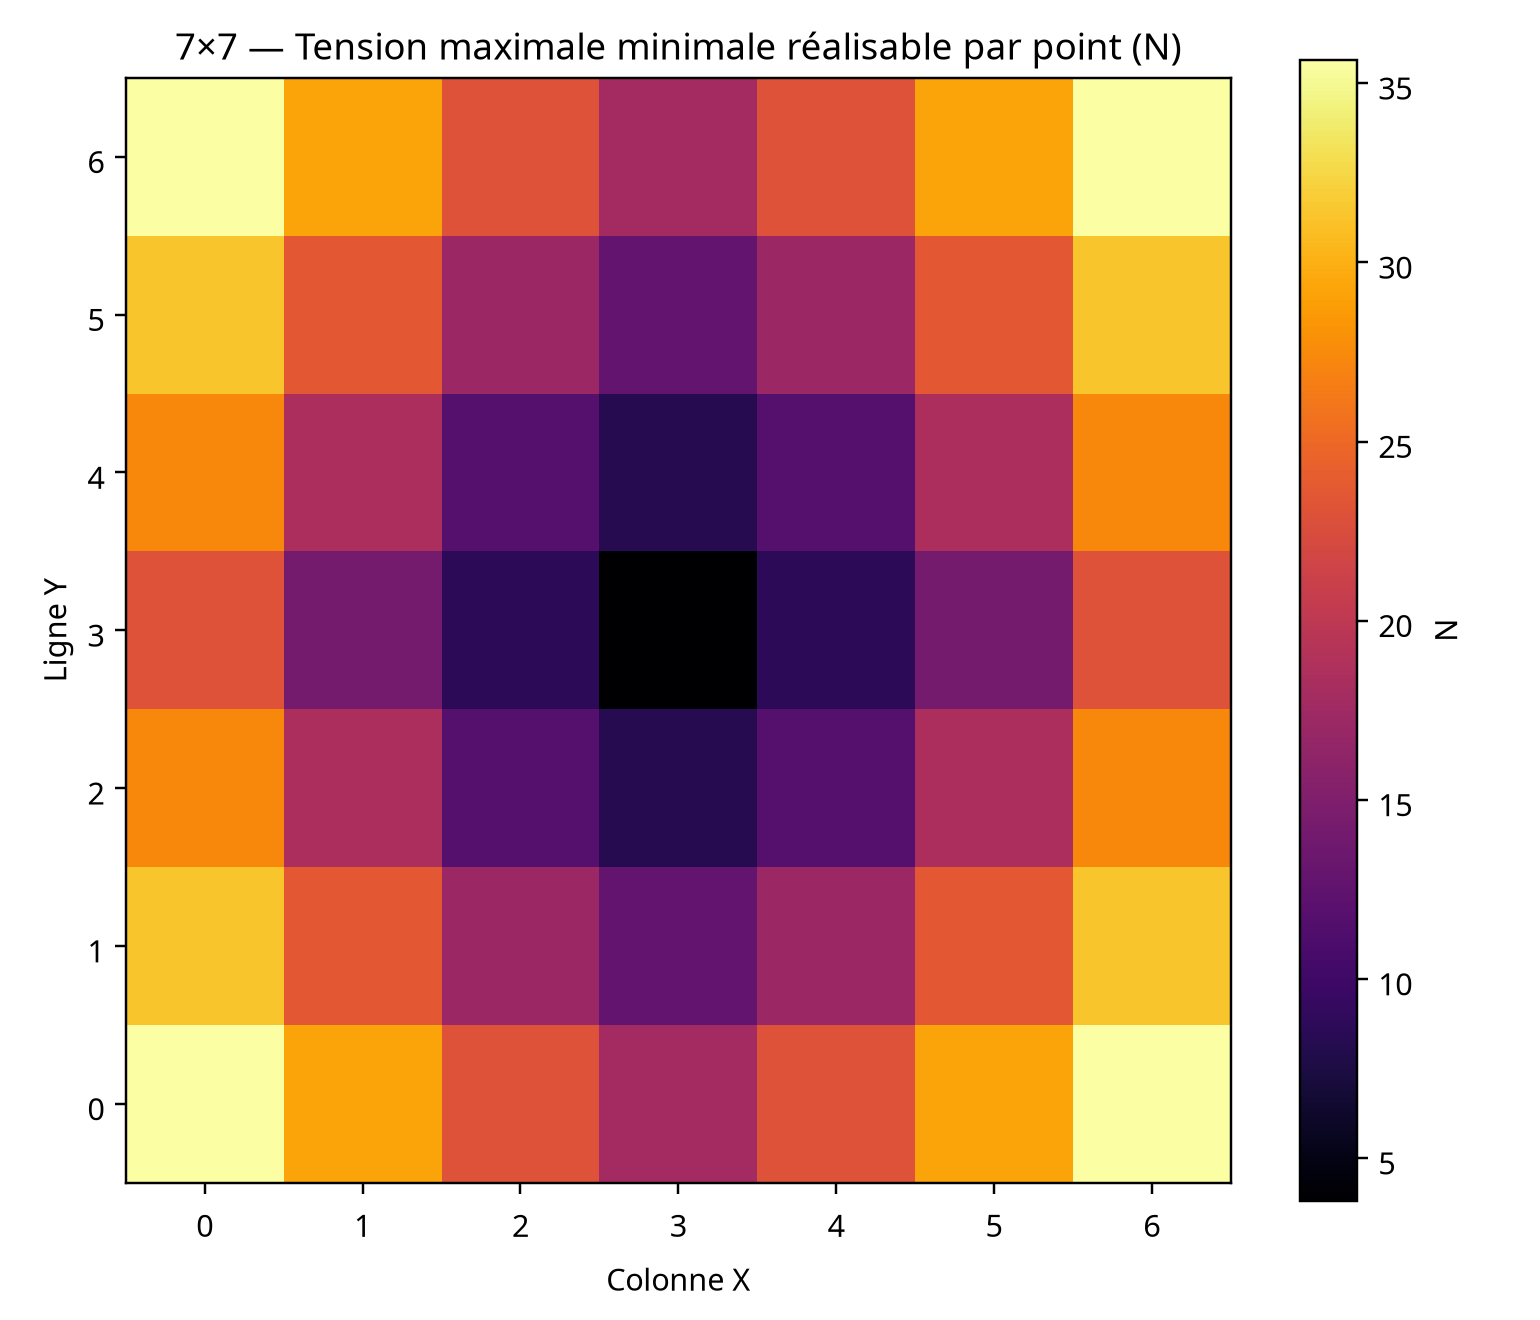
\includegraphics[width=\textwidth]{tens_maxmin.png}
\end{minipage}\hfill
\begin{minipage}{0.48\textwidth}
\centering
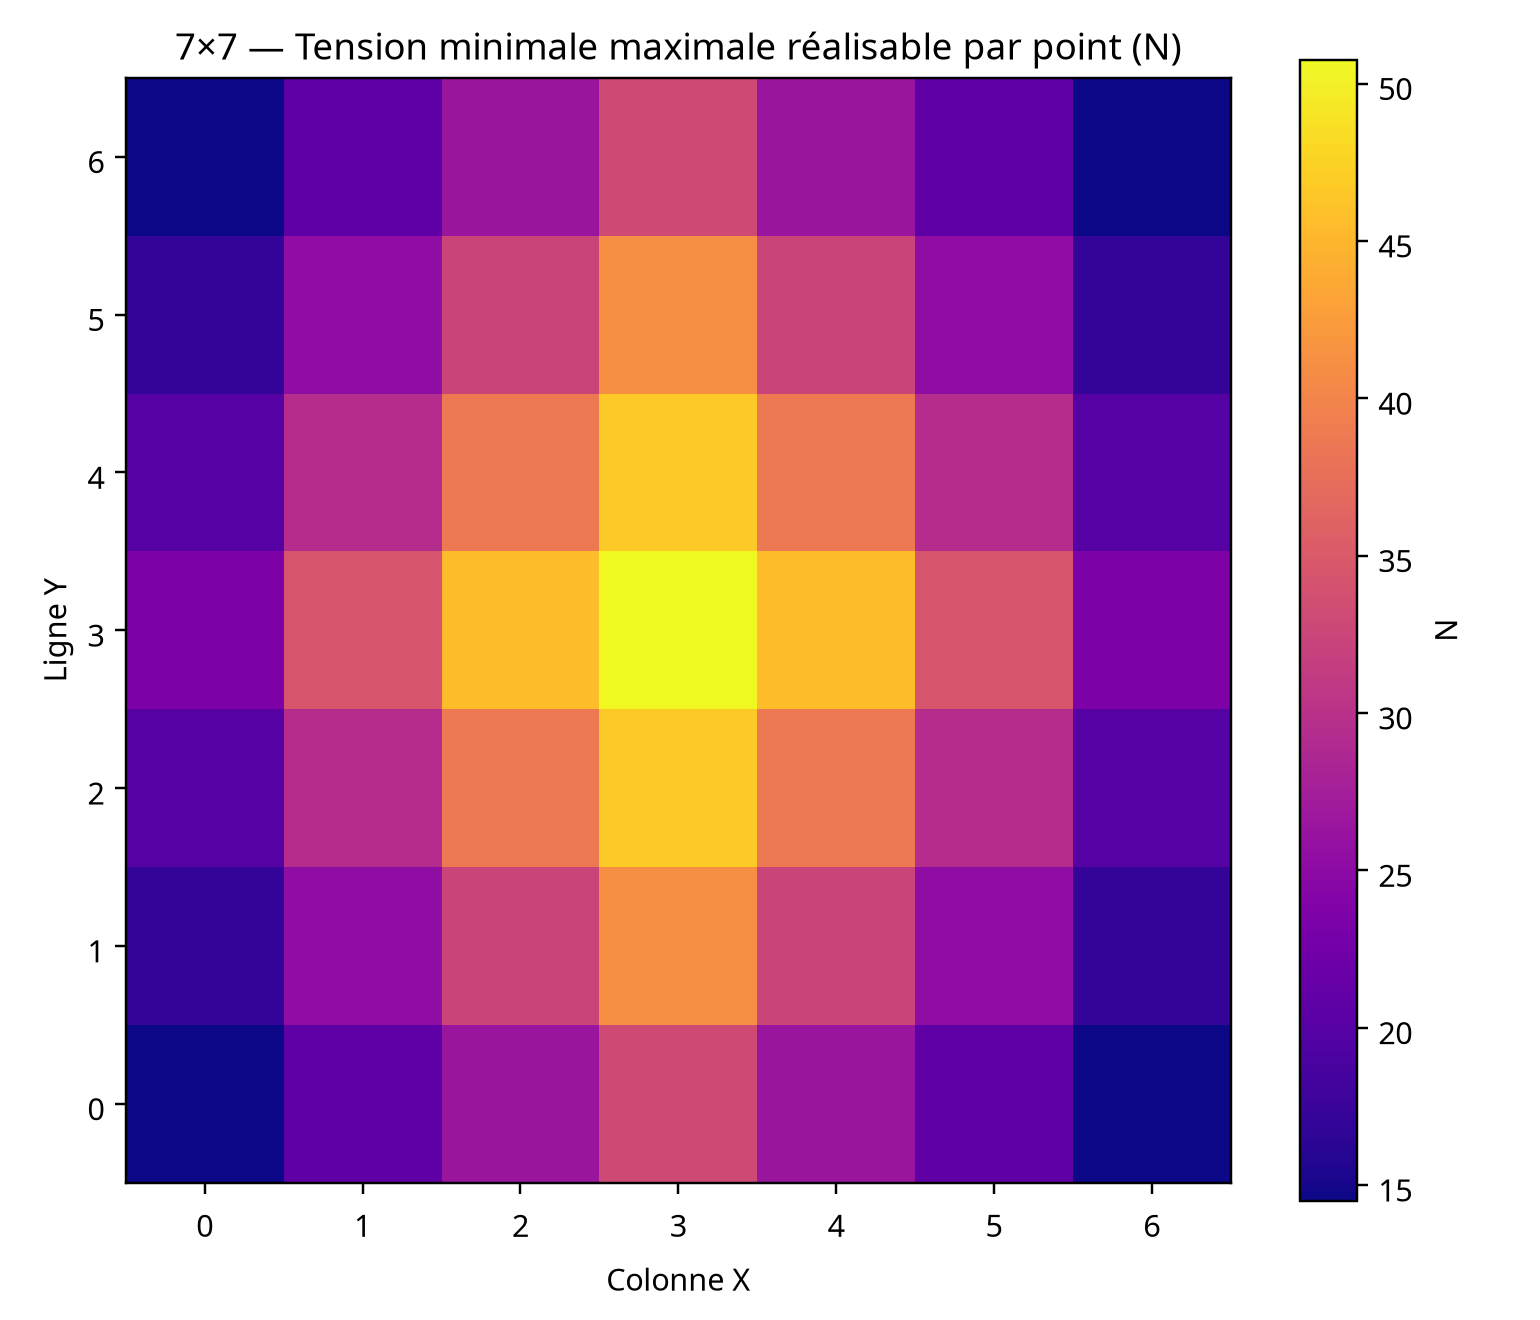
\includegraphics[width=\textwidth]{tens_minmax.png}
\end{minipage}
\caption{Tension des câbles par point pour grille $7\times7$}
\label{fig:tension}
\end{figure}

La répartition spatiale des tensions met en évidence un gradient marqué : minimale au centre (3,8~N), la tension requise augmente fortement vers les bords de la grille (jusqu'à 35,7~N) en raison de l'éloignement des ancrages. Cette élévation valide la robustesse de l'approche, les tensions maximales restant largement inférieures à la limite de sécurité de 58~N.


Sur la zone sécurisée $7\times7$, la tension maximale minimale varie de 3,8~N au centre à 35,7~N au bord (marge de 22,3~N sous la limite de 58~N).

\subsection{Effet de la couverture de la zone de travail}

Sur la grille $7\times7$ étendue : temps minimal 191,83~s / 315,61~J (gain 22,9~\% / 25,5~\% face au zigzag). Sur la grille $9\times9$ étendue (77 points) : temps minimal 301,15~s, énergie 636,65~J (gains 2,0~\% / 2,7~\% face au plus proche voisin).

\begin{figure}[H]
\centering
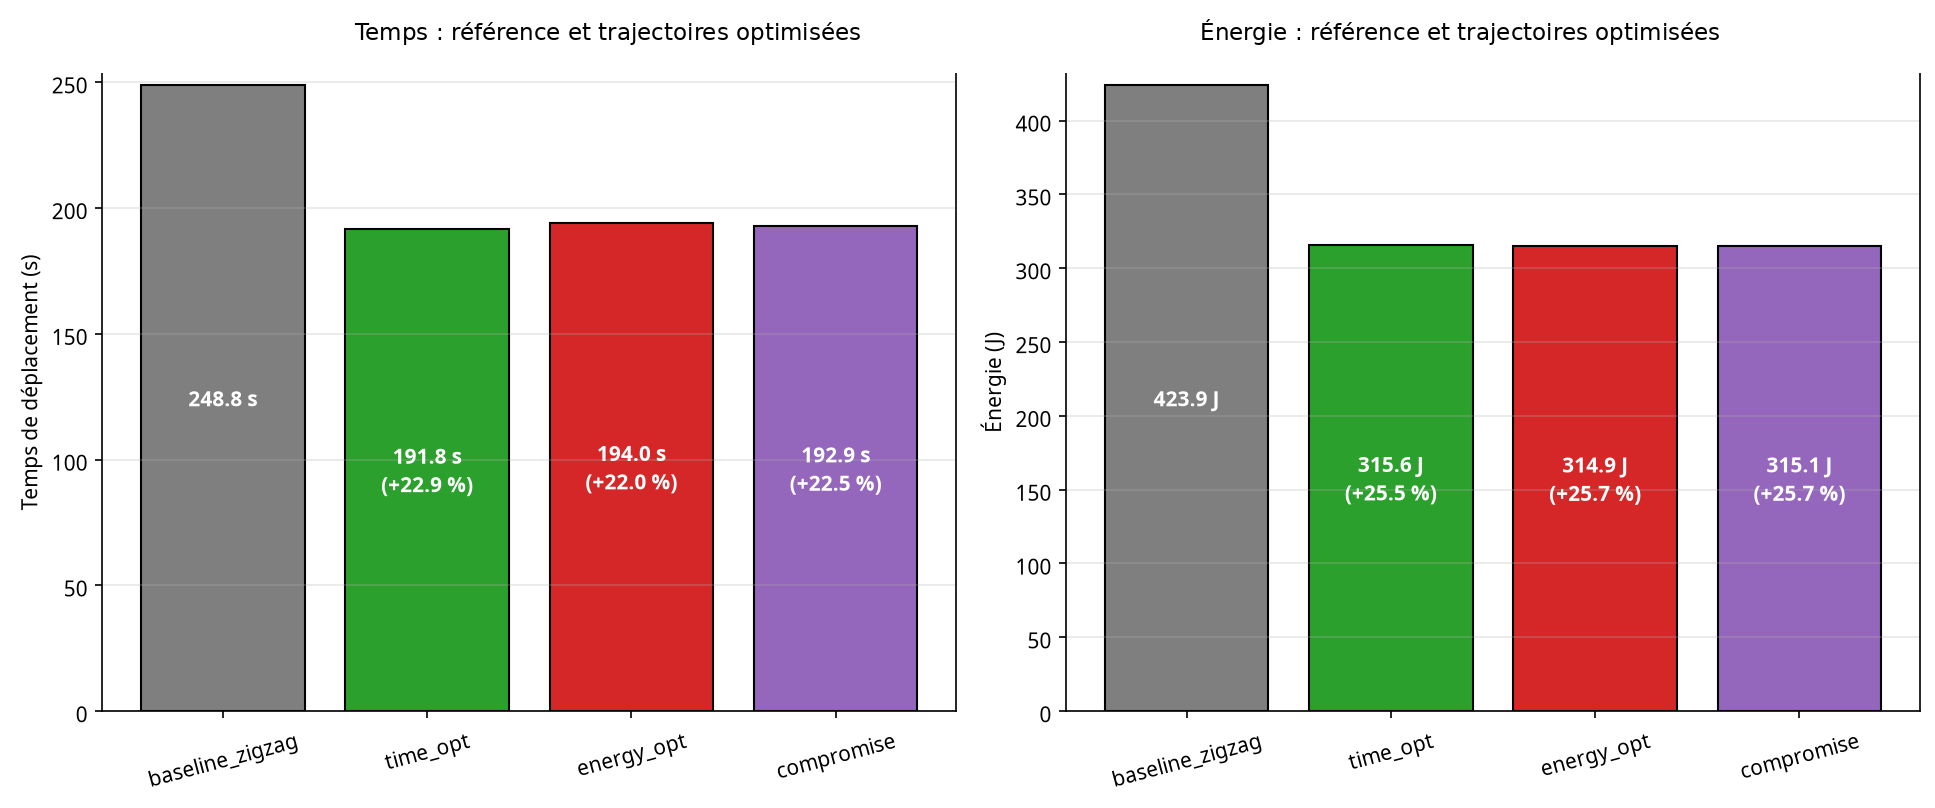
\includegraphics[width=0.92\textwidth,height=0.34\textheight,keepaspectratio]{comp_ext_7x7.png}\\[0.3em]
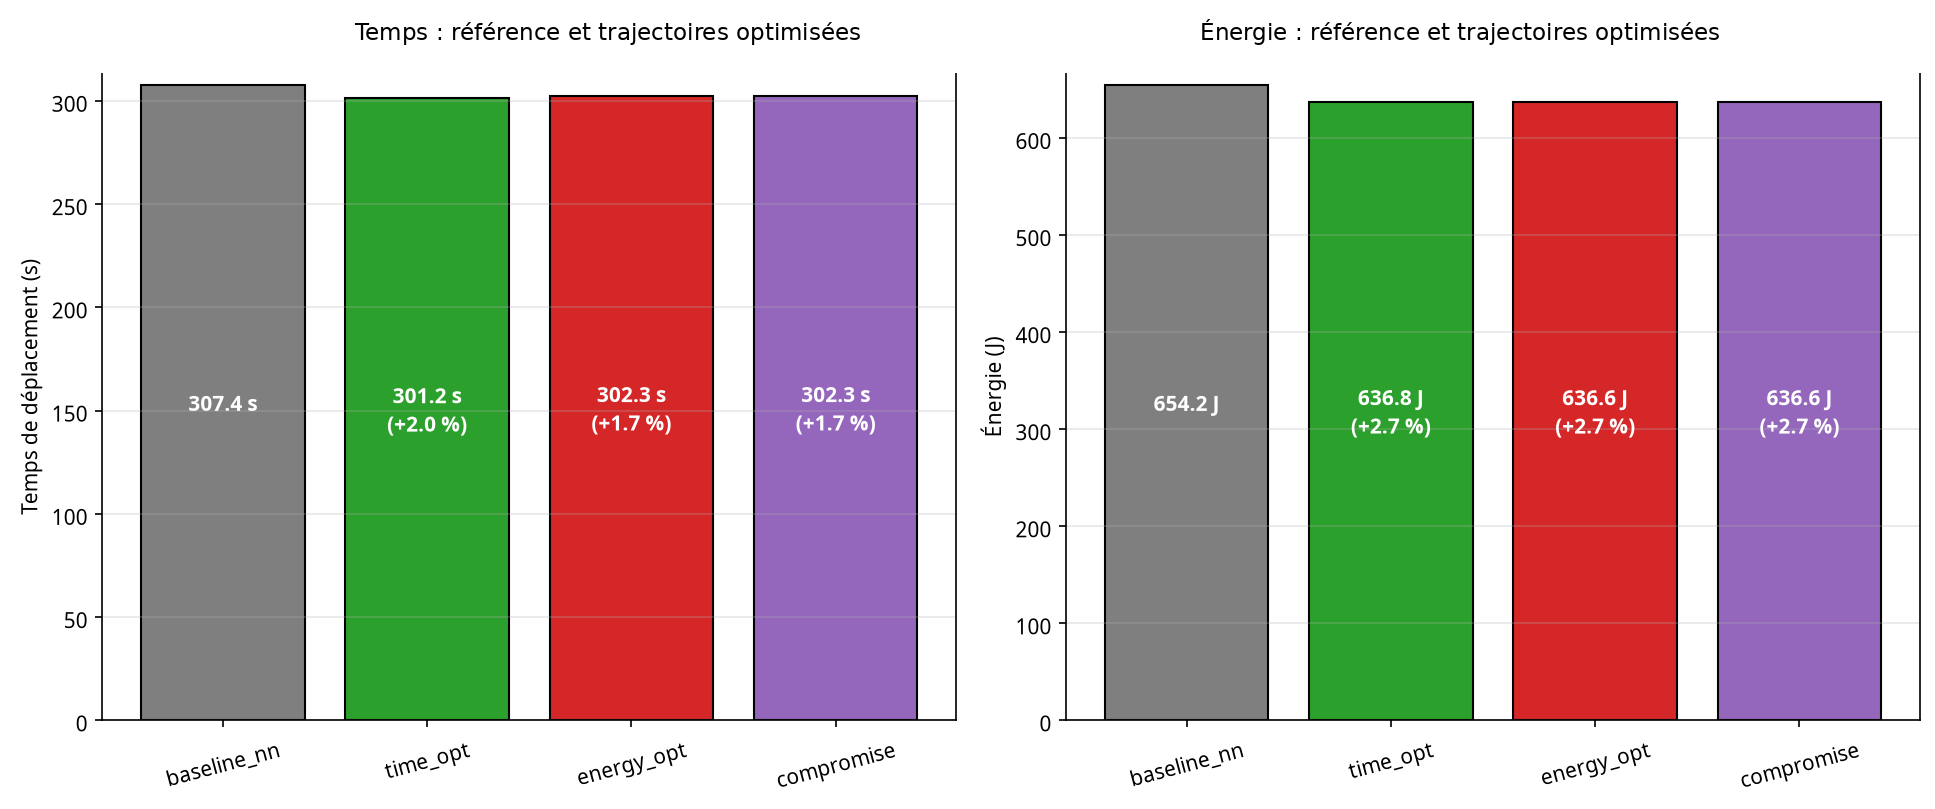
\includegraphics[width=0.92\textwidth,height=0.34\textheight,keepaspectratio]{comp_ext_9x9.png}
\caption{Temps et énergie, zone étendue}
\label{fig:comp_ext}
\end{figure}

\begin{figure}[H]
\centering
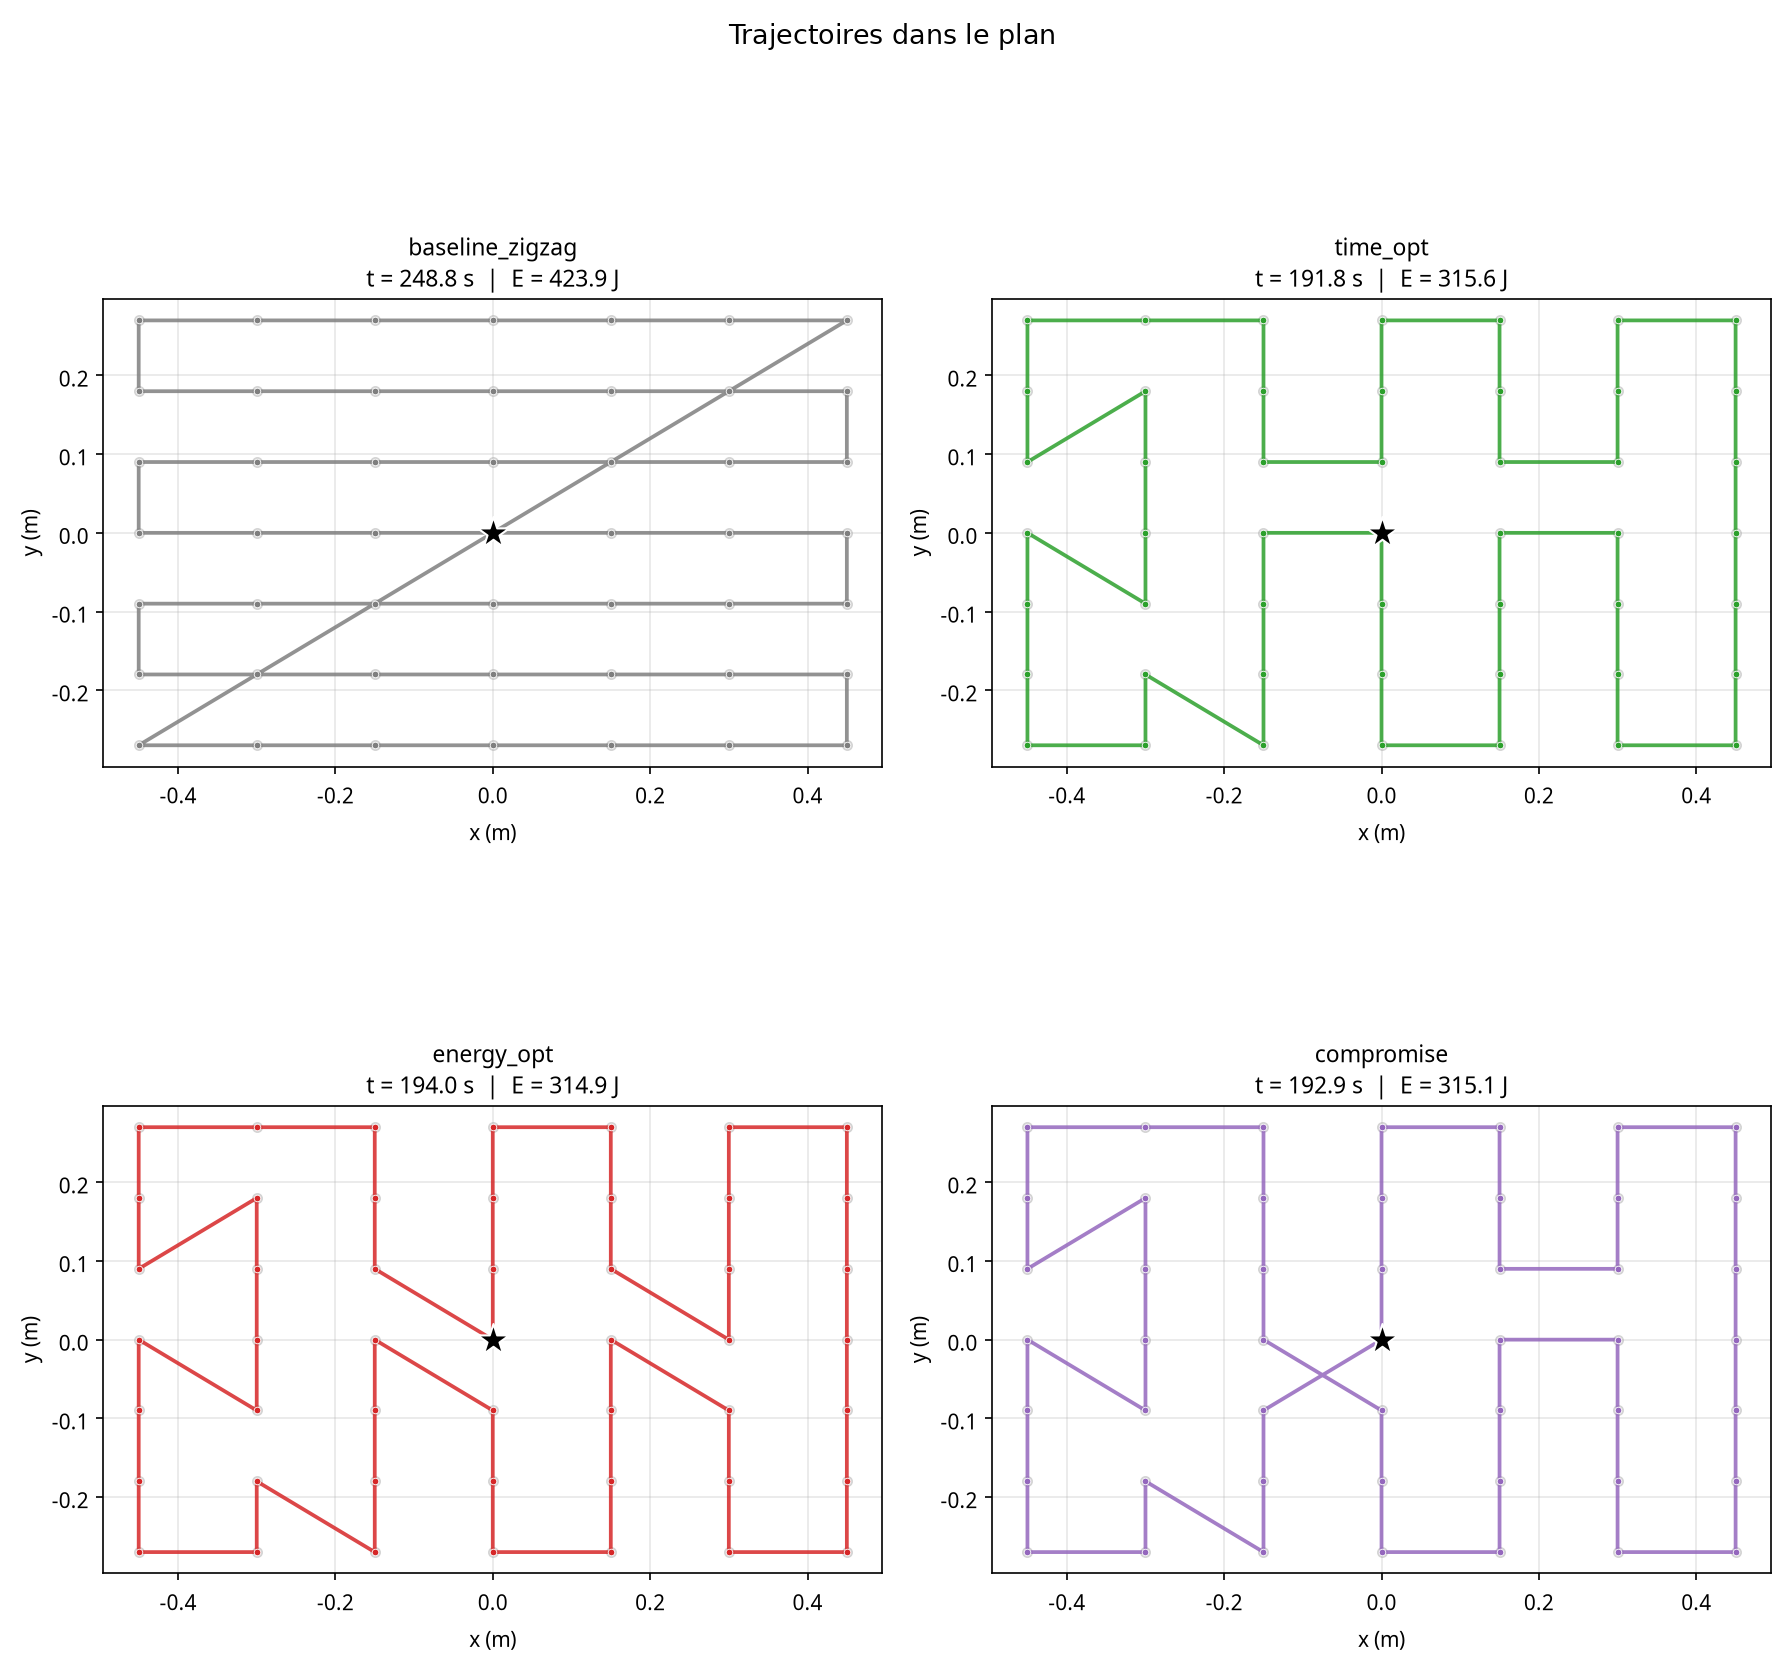
\includegraphics[width=\textwidth,height=0.78\textheight,keepaspectratio]{traj_ext_7x7.png}
\caption{Tracé 2D des trajectoires, zone étendue — grille $7\times7$}
\label{fig:traj_ext_7}
\end{figure}

Le tracé comparatif met en évidence la supériorité des chemins optimisés (vert, rouge, violet) sur la baseline en zigzag (gris). On observe que l'algorithme évite les allers-retours systématiques et les croisements inutiles, réduisant ainsi la distance globale parcourue. Cette visualisation confirme le gain de 22,9~\% en temps : NSGA-II exploite efficacement l'espace élargi en trouvant un ordre de visite beaucoup plus fluide.


\begin{figure}[H]
\centering
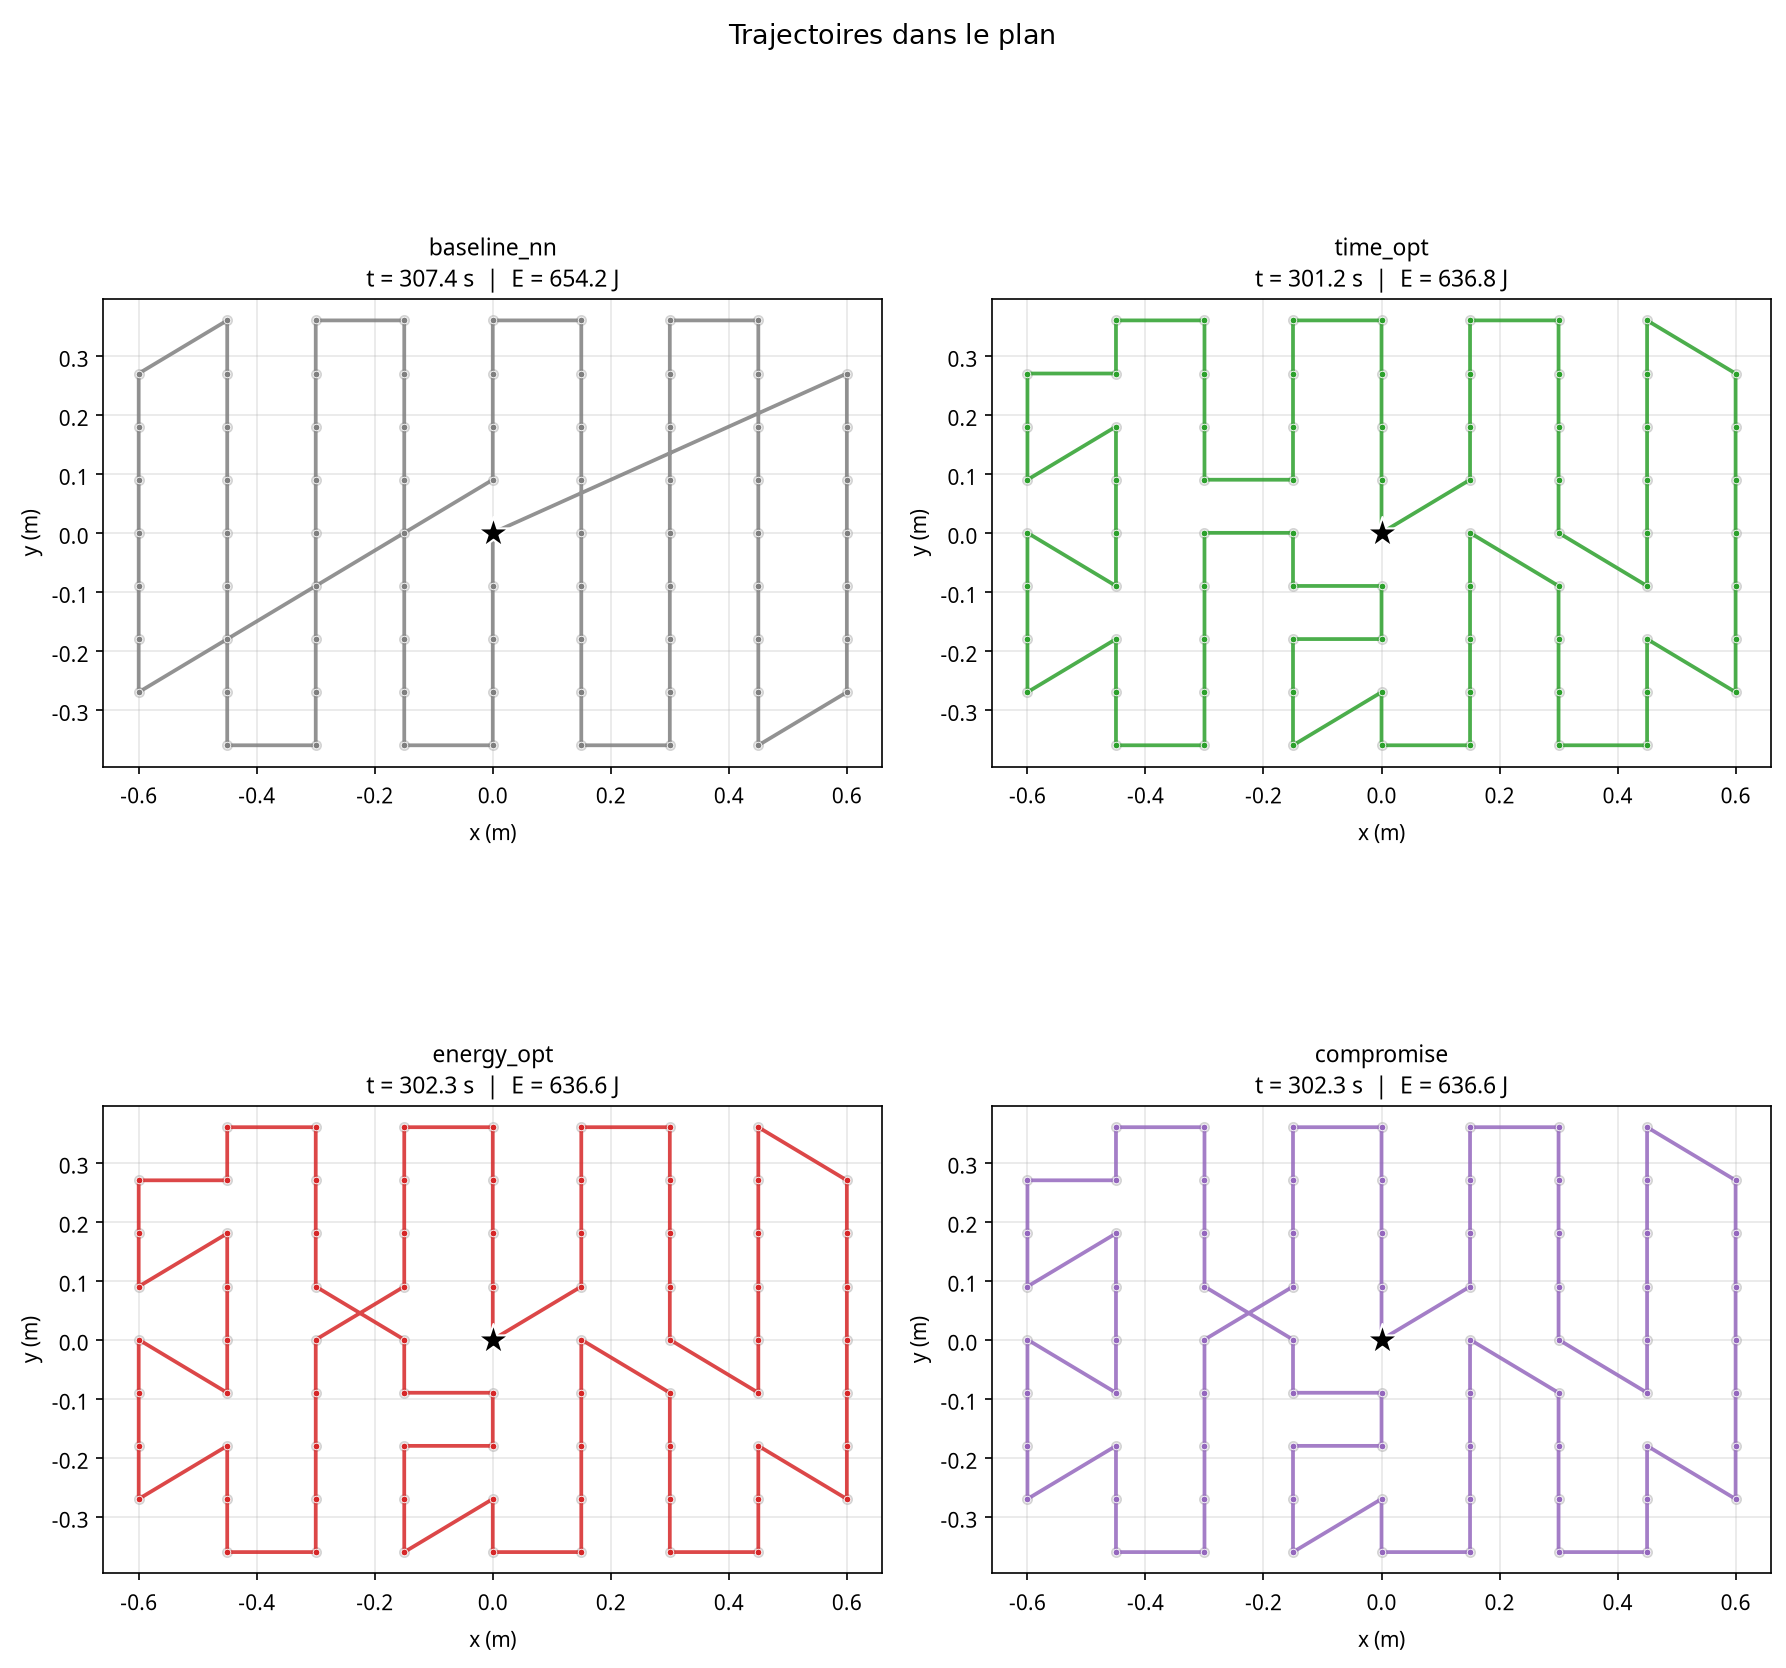
\includegraphics[width=\textwidth,height=0.78\textheight,keepaspectratio]{traj_ext_9x9.png}
\caption{Tracé 2D des trajectoires, zone étendue — grille $9\times9$}
\label{fig:traj_ext_9}
\end{figure}

La représentation de la grille $9\times9$ étendue (77 points, coins rejetés) révèle des trajectoires optimisées plus denses et complexes. Contrairement à la grille $7\times7$, les gains face à la baseline sont marginaux (2,0~\% en temps), car le balayage colonne par colonne est déjà naturellement proche de l'optimum pour un maillage aussi fin. L'optimisation démontre néanmoins sa capacité à gérer des espaces non convexes en contournant les quatre coins infaisables tout en maintenant un trajet cohérent et sans croisement.


\begin{figure}[H]
\centering
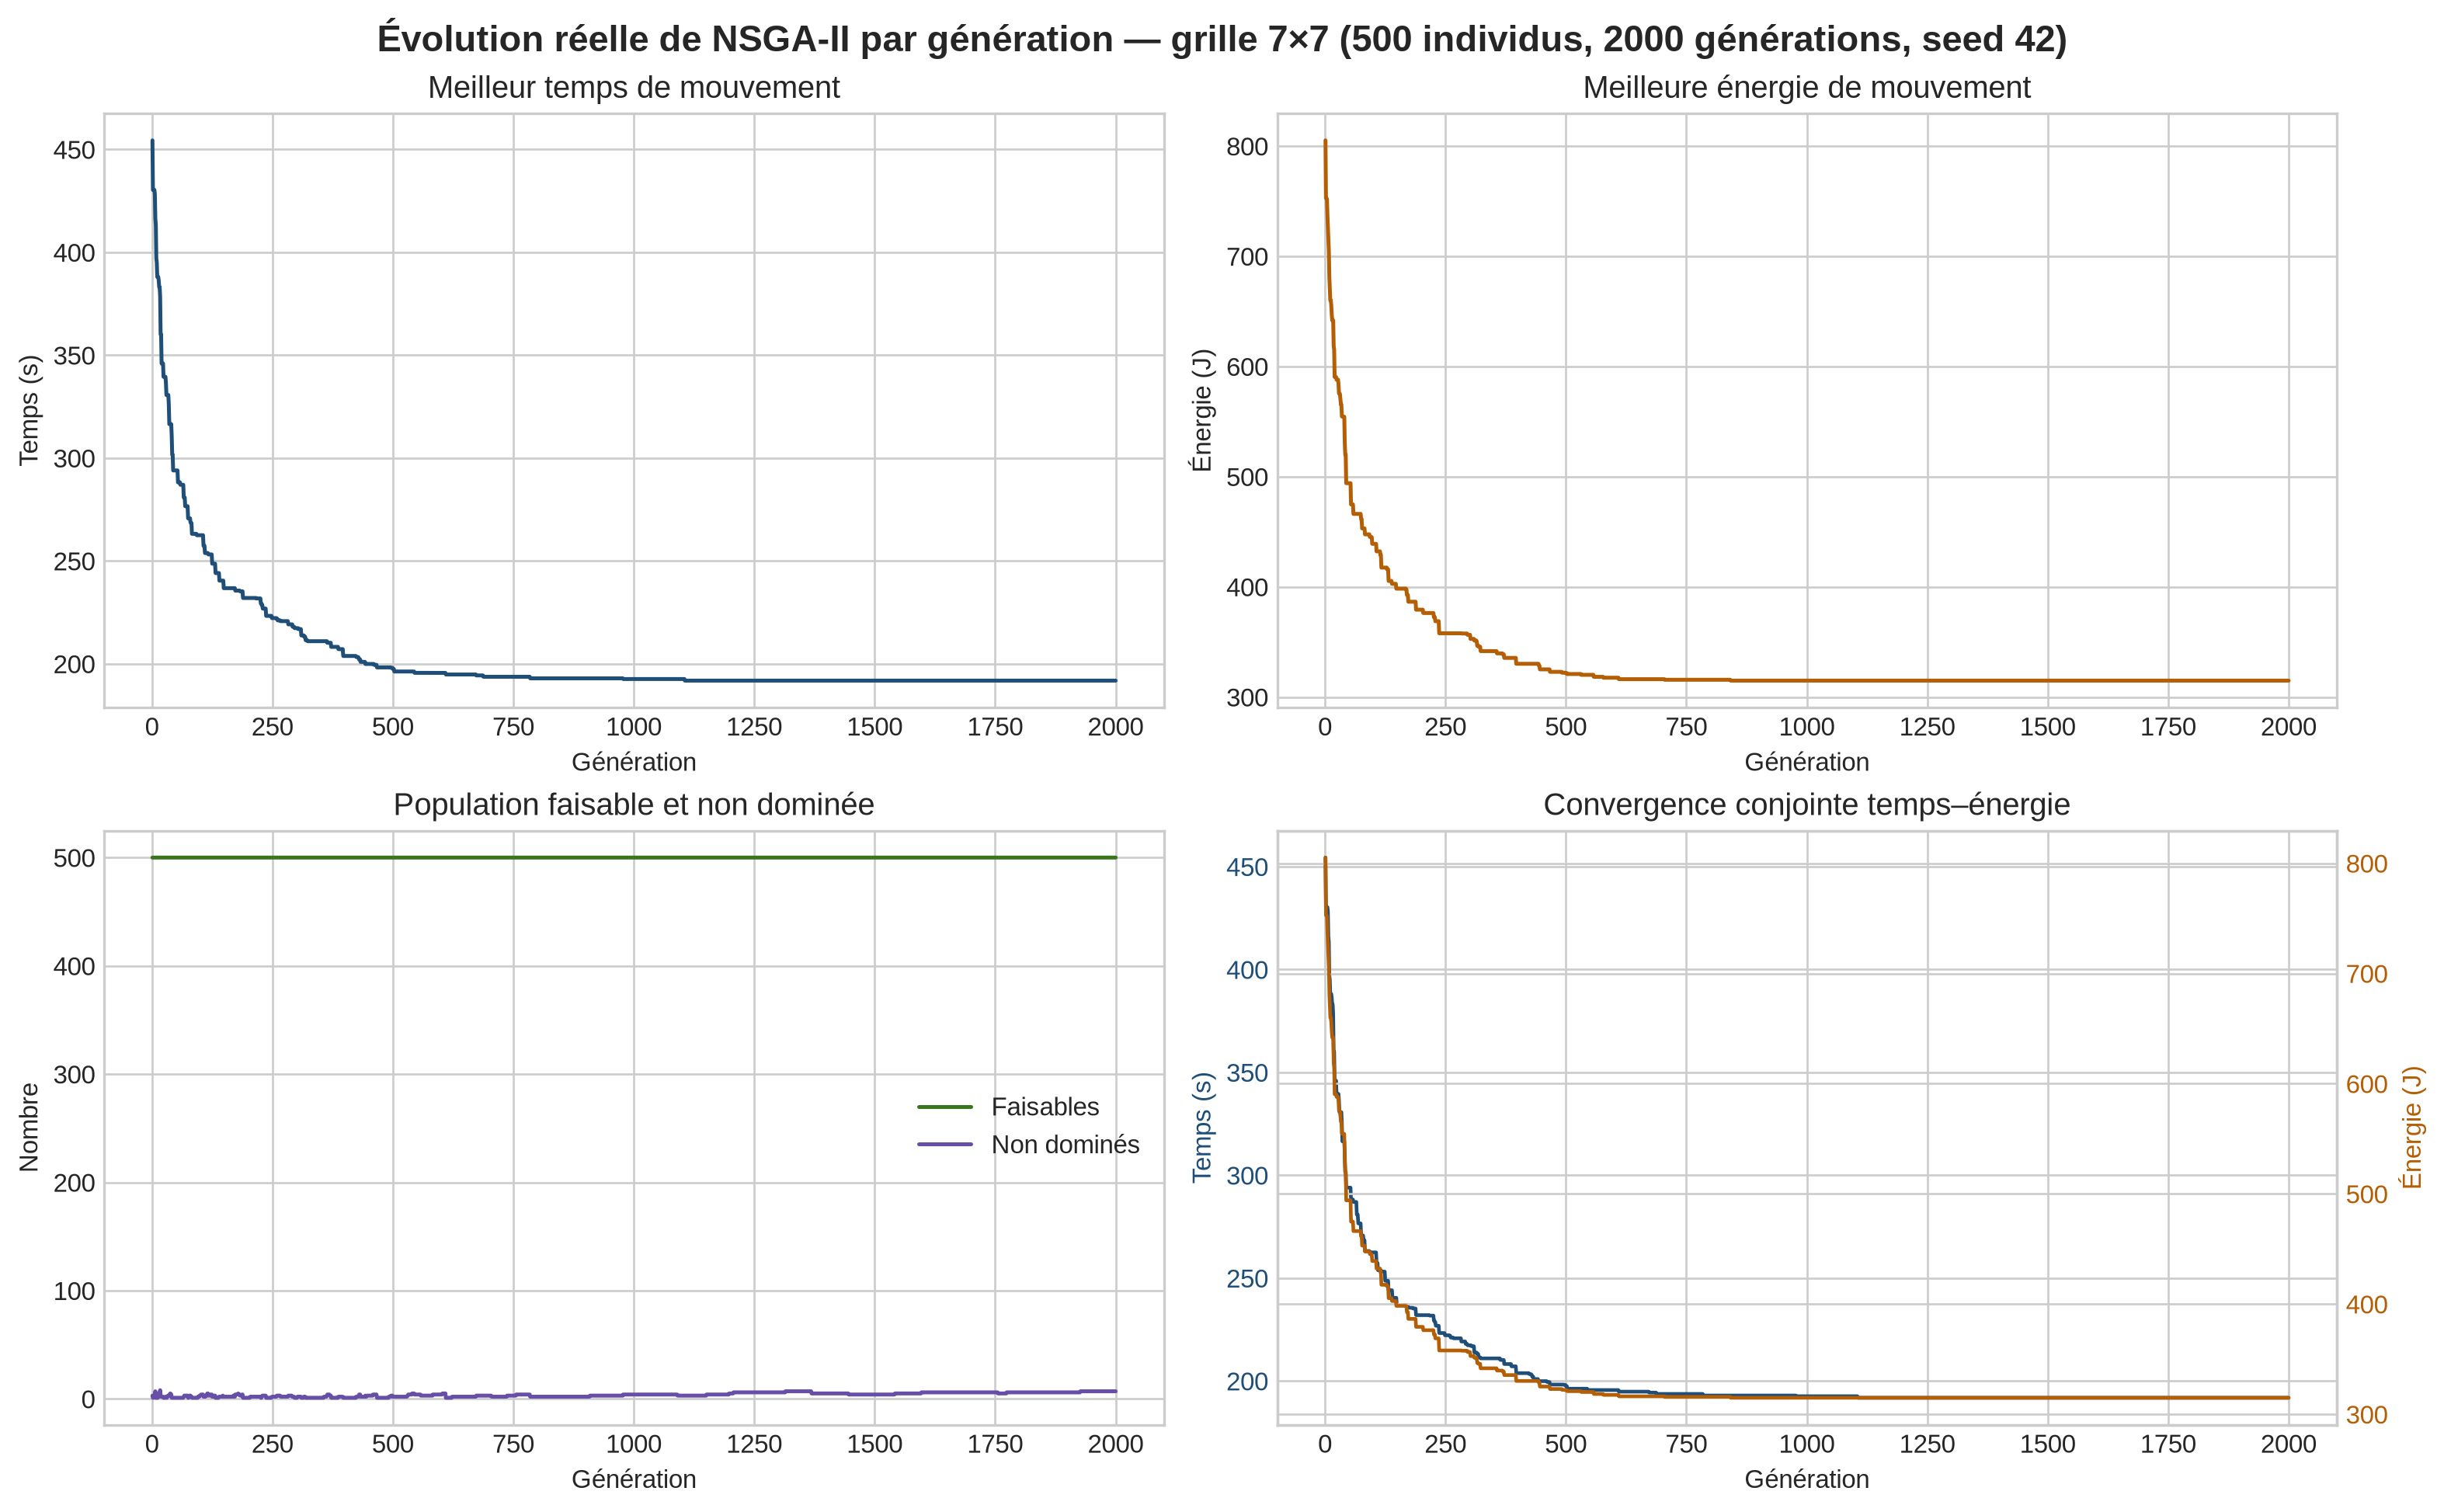
\includegraphics[width=0.95\textwidth,height=0.42\textheight,keepaspectratio]{conv_7x7.png}\\[0.35em]
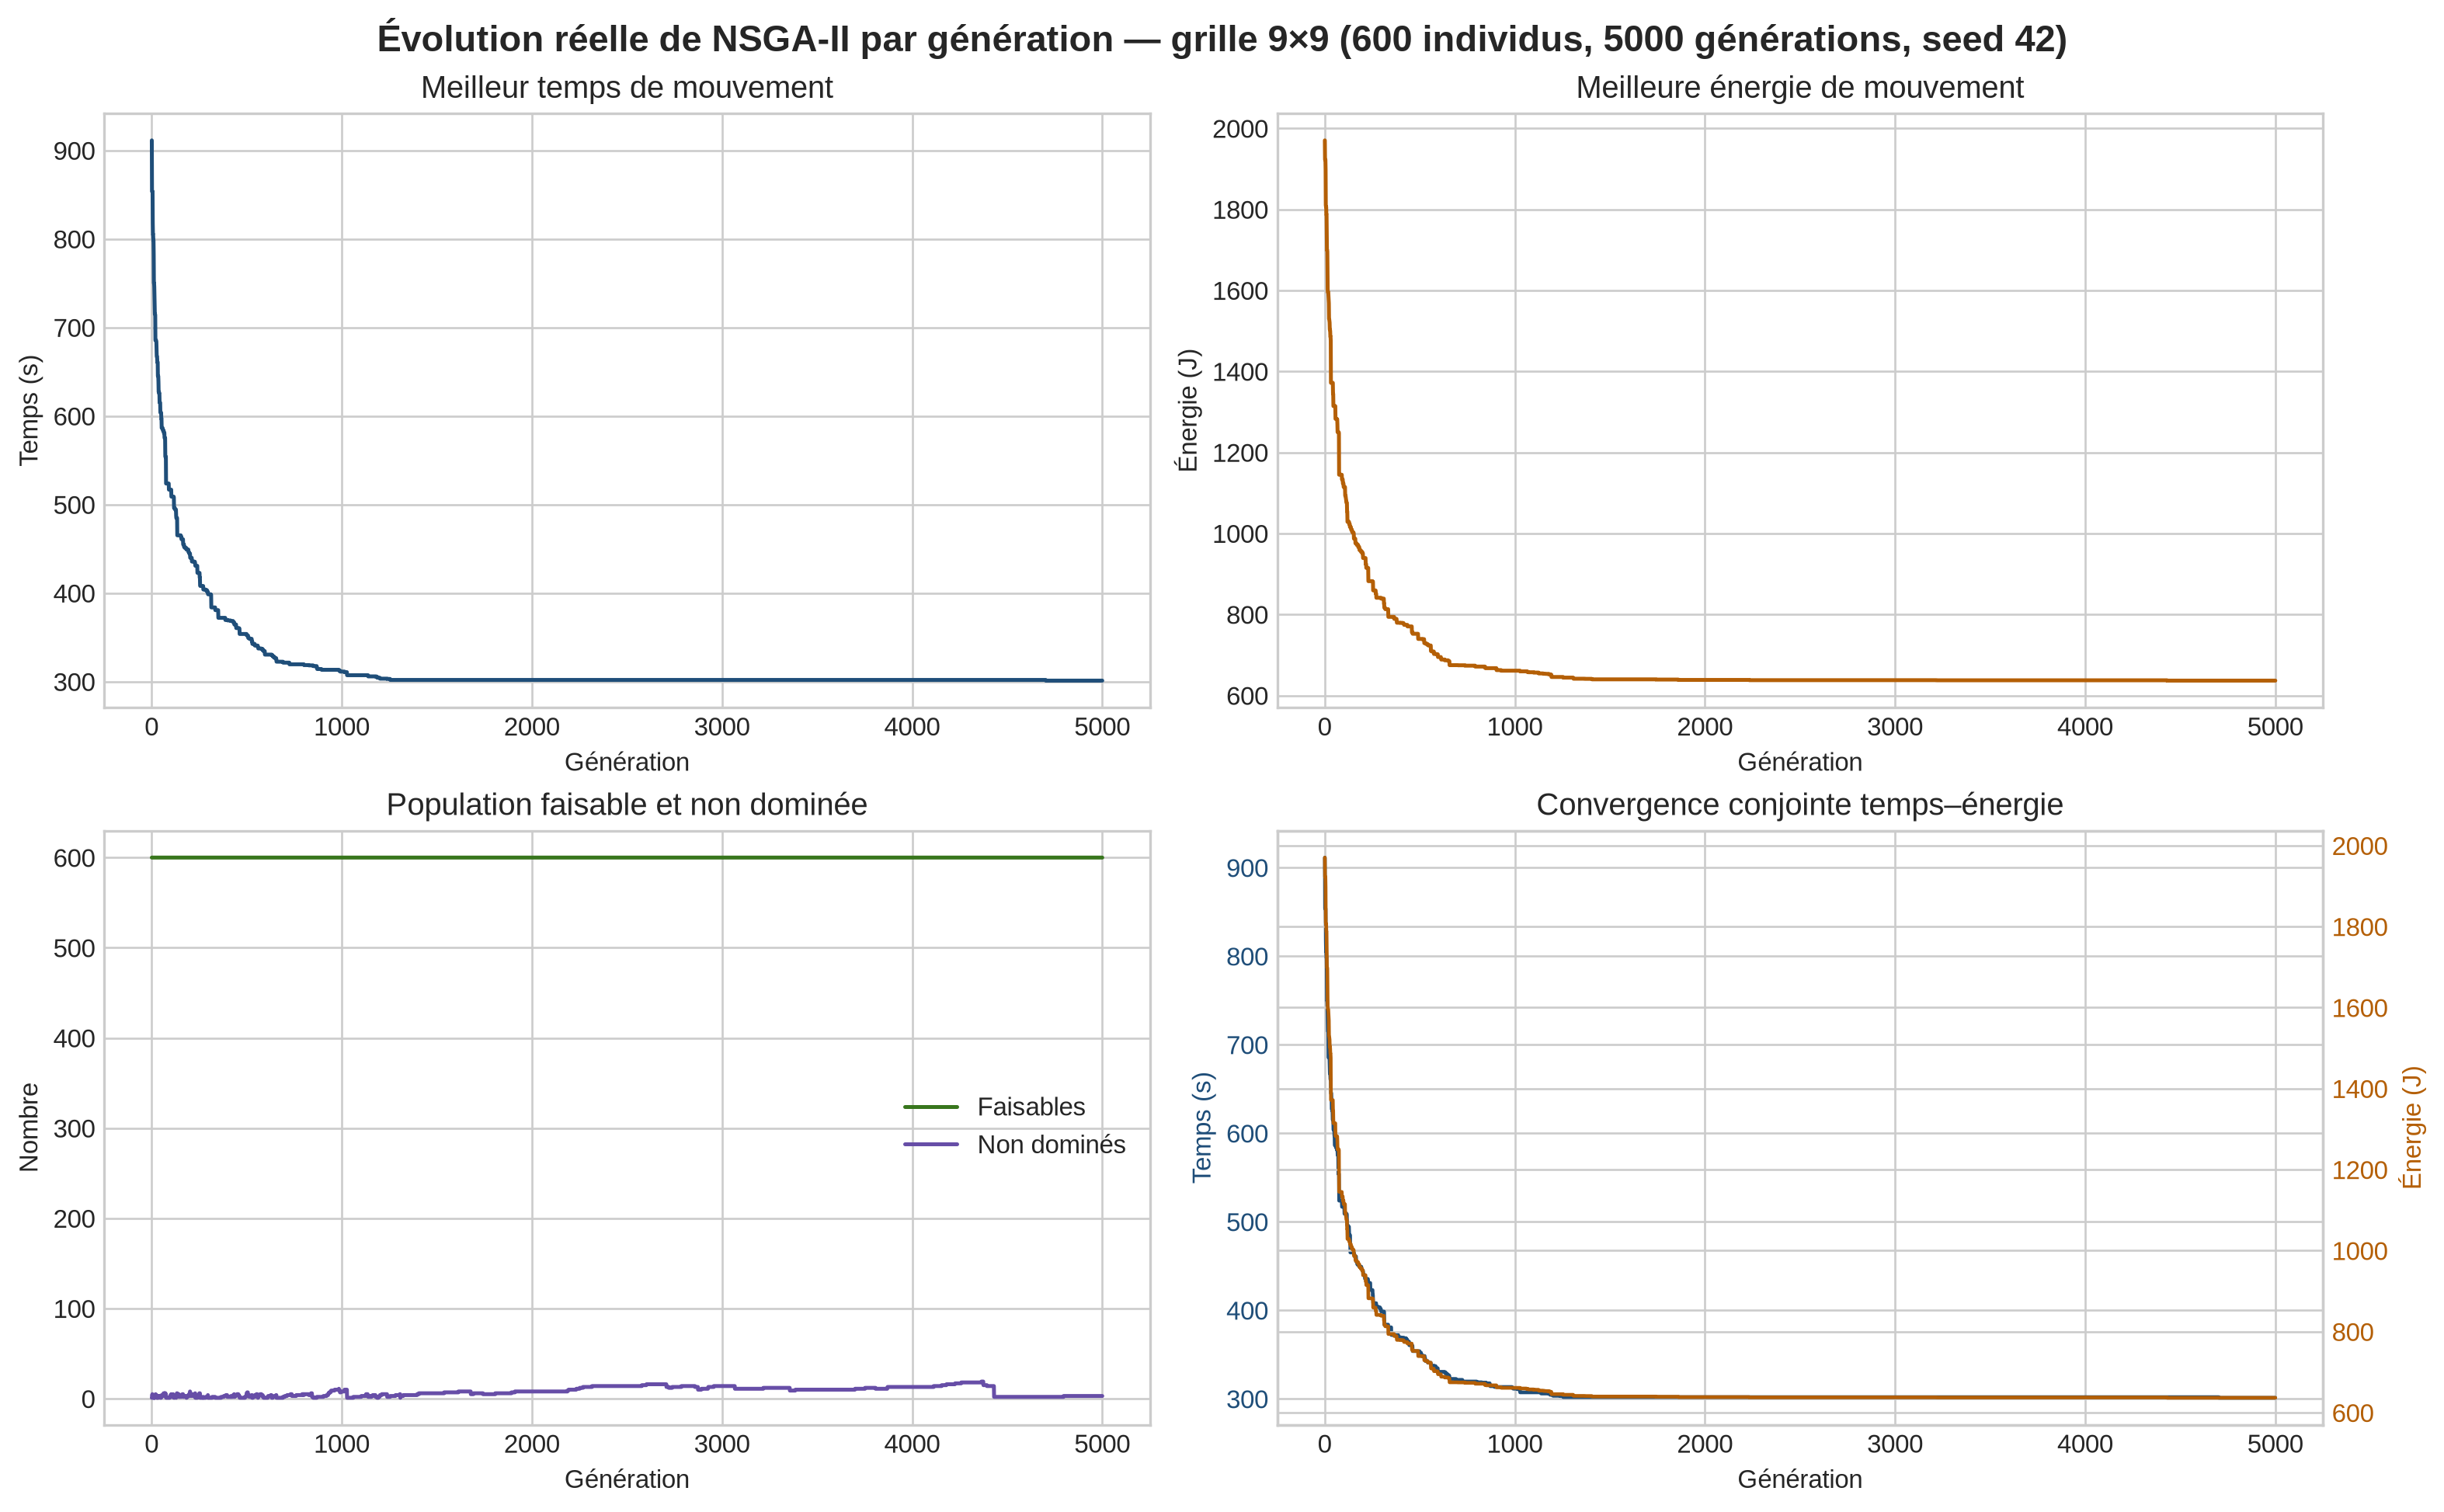
\includegraphics[width=0.95\textwidth,height=0.42\textheight,keepaspectratio]{conv_9x9.png}
\caption{Convergence de NSGA-II, zone étendue : (a) grille $7\times7$, (b) grille $9\times9$}
\label{fig:conv}
\end{figure}

L'évolution de l'algorithme au fil des générations est marquée par une chute rapide des coûts (temps et énergie), suivie d'un plateau asymptotique, tandis que la population maintient un taux de faisabilité de 100~\%. Cette dynamique confirme que les nombres de générations retenus (2000 et 5000) sont amplement suffisants pour atteindre l'optimum sans calculs superflus.


\begin{figure}[H]
\centering
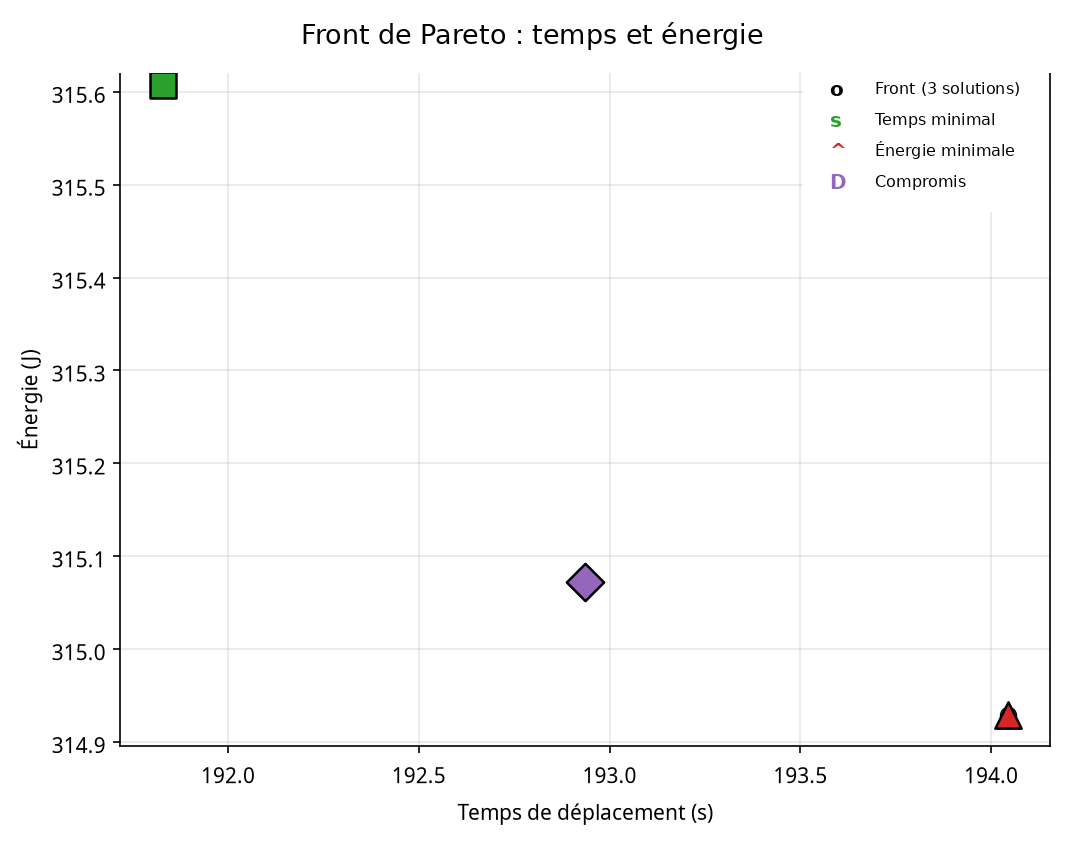
\includegraphics[width=0.92\textwidth,height=0.34\textheight,keepaspectratio]{pareto_7x7.png}\\[0.3em]
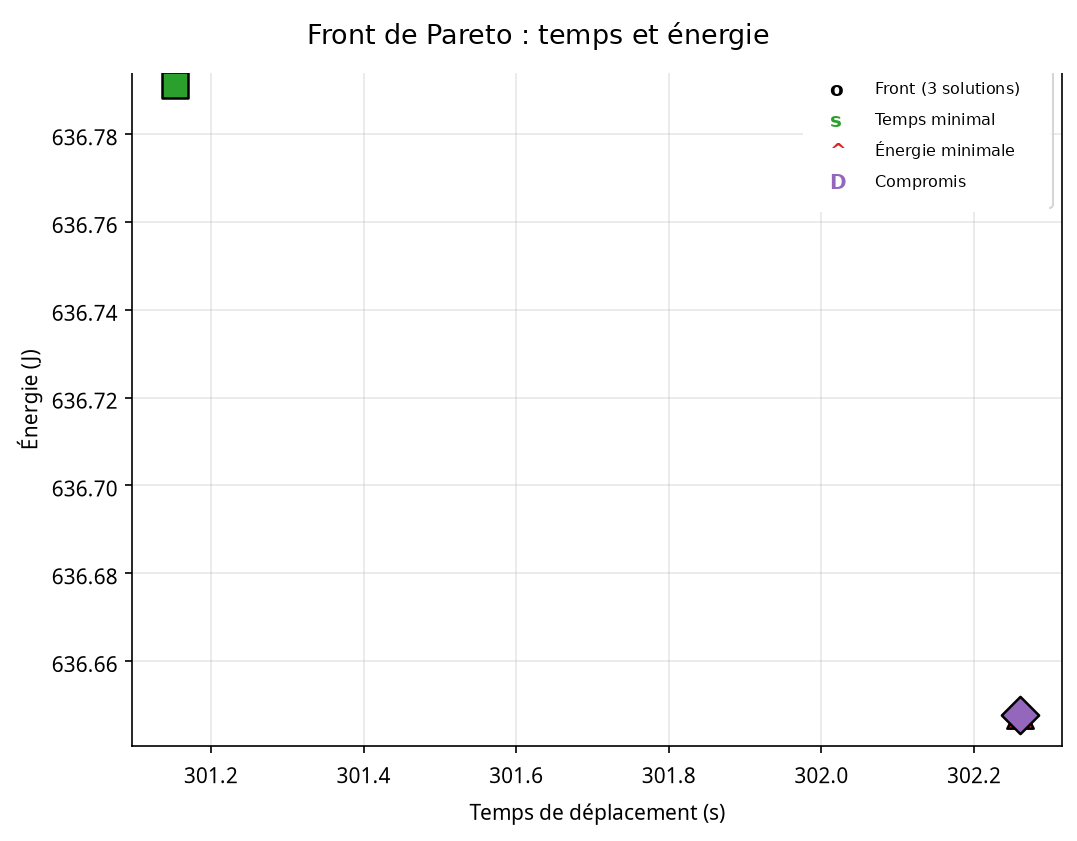
\includegraphics[width=0.92\textwidth,height=0.34\textheight,keepaspectratio]{pareto_9x9.png}
\caption{Fronts de Pareto temps--énergie, zone étendue}
\label{fig:pareto}
\end{figure}

L'analyse du front de Pareto révèle que les trois solutions optimales (temps minimal, énergie minimale et compromis) sont extrêmement proches les unes des autres. Cela démontre que, pour cette configuration, minimiser le temps ne dégrade pas significativement l'énergie, ce qui simplifie le choix de la trajectoire finale.


\begin{figure}[H]
\centering
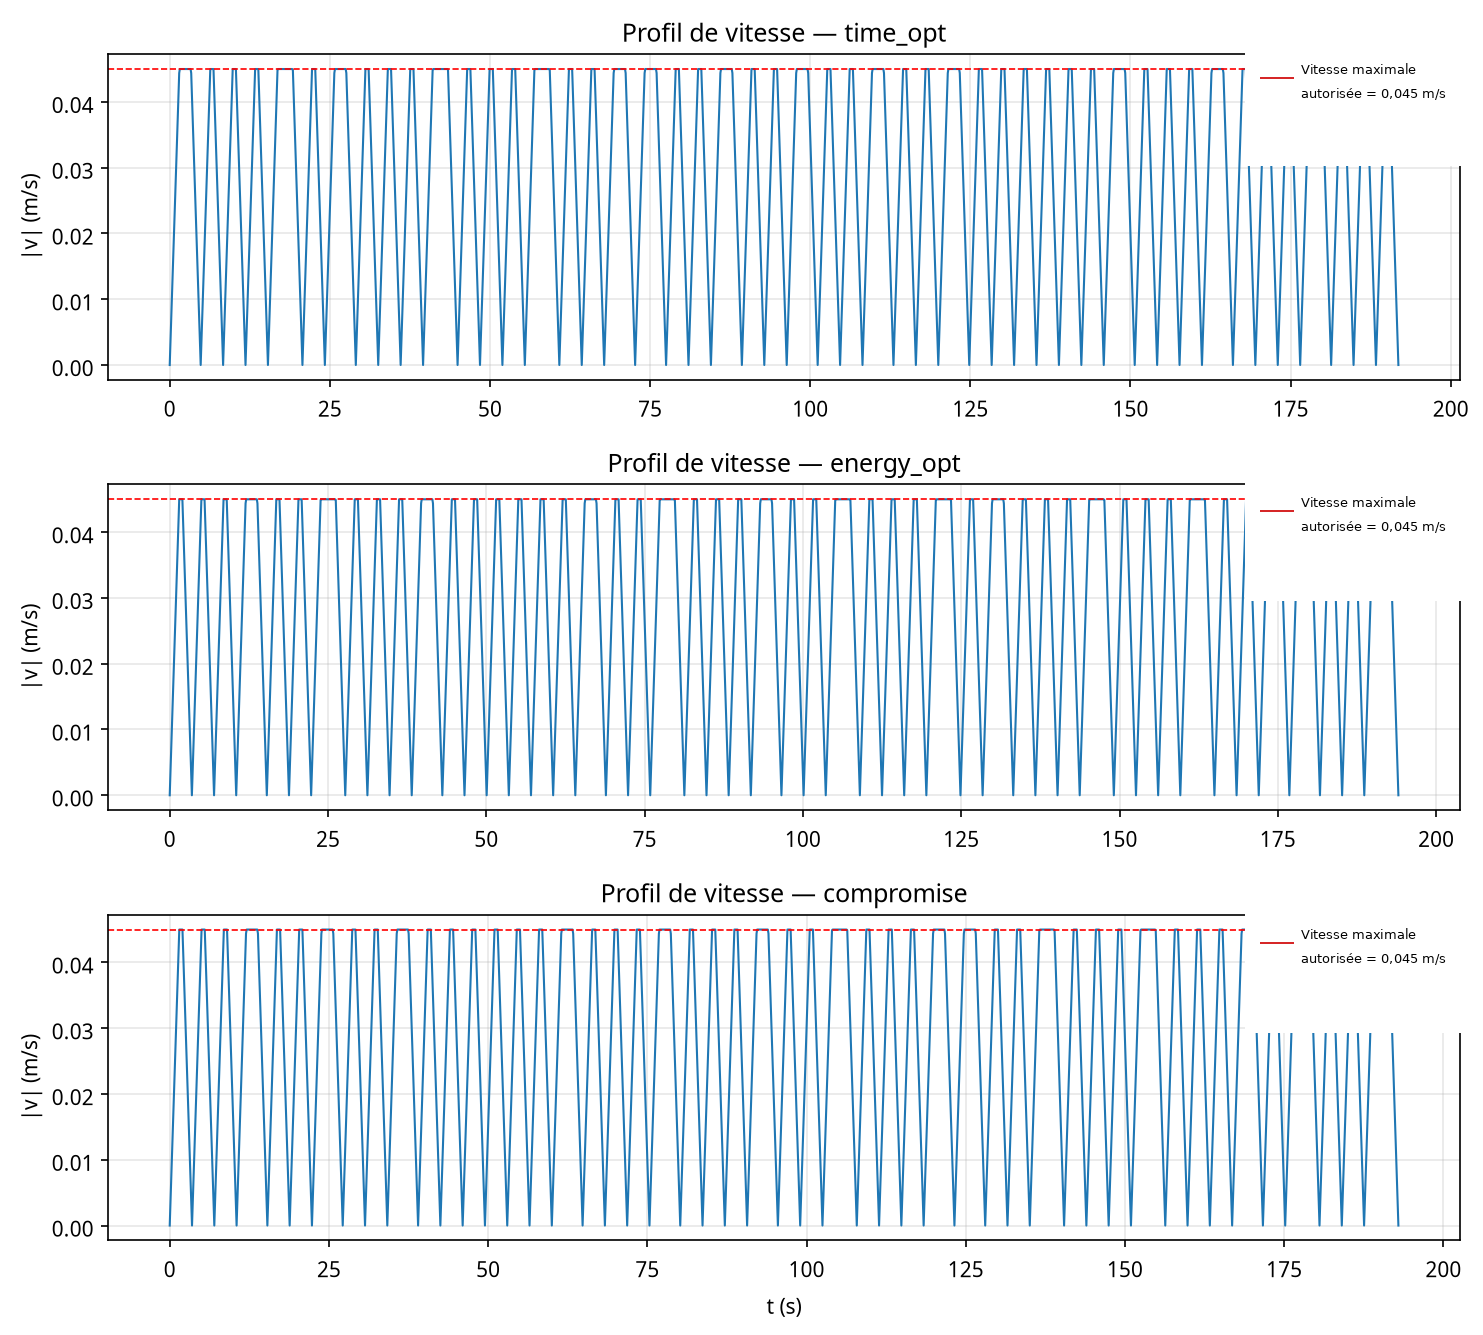
\includegraphics[width=0.92\textwidth,height=0.34\textheight,keepaspectratio]{prof_7x7.png}\\[0.3em]
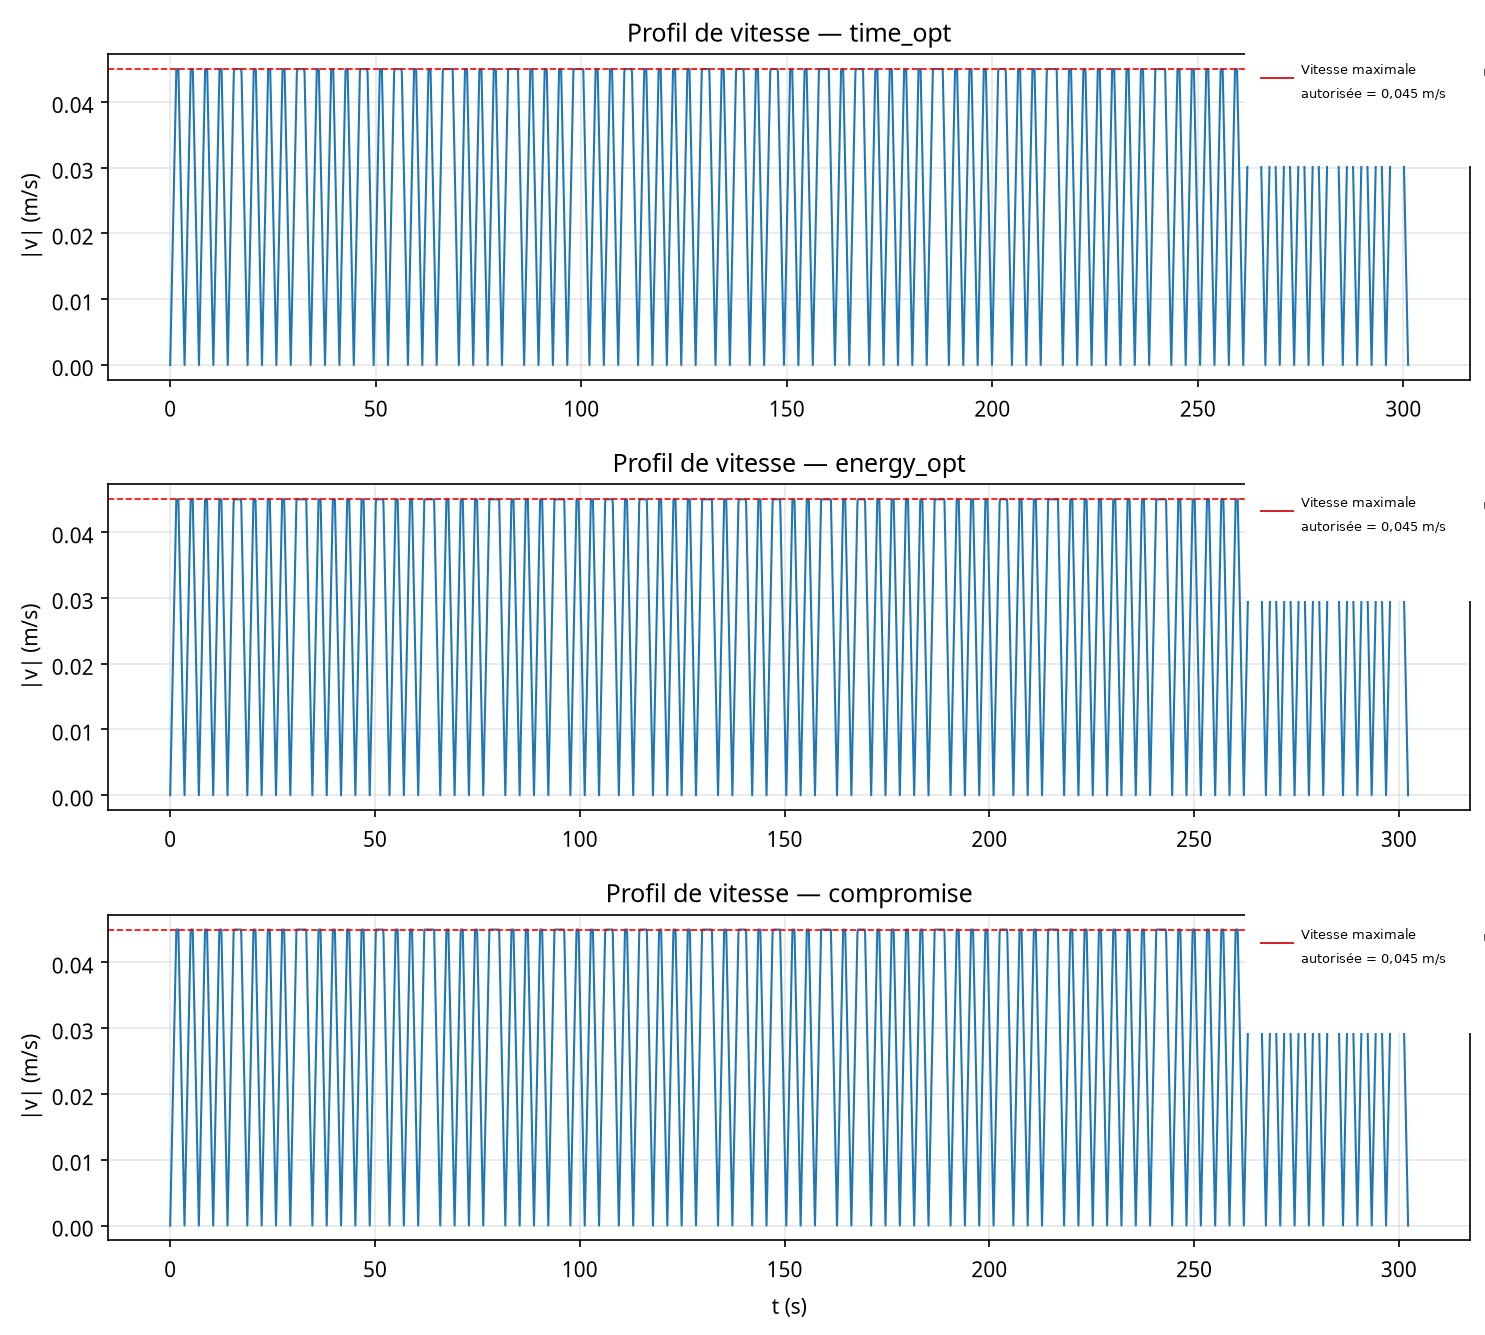
\includegraphics[width=0.92\textwidth,height=0.34\textheight,keepaspectratio]{prof_9x9.png}
\caption{Profils de vitesse LSPB des trois trajectoires, zone étendue}
\label{fig:prof}
\end{figure}

\begin{table}[H]
\centering
\caption{Comparaison zone sécurisée et zone étendue}
\label{tab:zones}
\footnotesize
\begin{tabular}{|c|c|c|c|c|c|}
\hline
\textbf{Grille} & \textbf{Zone} & \textbf{Points} & \textbf{Temps (s)} & \textbf{Énergie (J)} & \textbf{Total (s)} \\
\hline
$7\times7$ & Sécurisée & 49 & 177,30 & 246,44 & 275,3 \\
\hline
$7\times7$ & Étendue & 49 & 191,83 & 314,93 & 289,8 \\
\hline
$9\times9$ & Sécurisée & 81 & 247,04 & 294,09 & 409,0 \\
\hline
$9\times9$ & Étendue & 77 & 301,15 & 636,65 & 455,2 \\
\hline
\end{tabular}
\end{table}

Pour la grille $7\times7$, l'extension ajoute 8,2~\% de temps et 28~\% d'énergie. Pour la grille $9\times9$, elle ajoute 22~\% de temps et 116~\% d'énergie. La zone sécurisée est retenue comme zone de service.

\section{Discussion et perspectives}

\subsection{Limites}

Résultats issus de simulations (câbles rigides, pas de vent, énergie quasi-statique). Paramètres à confirmer : masse opérationnelle, $T_{\max}=58$~N, stabilisation de 2~s. WFW étudié uniquement au plan $z=0{,}45$~m. Robustesse évaluée sur trois graines. Front de Pareto réduit en zone sécurisée. Aucune validation sur prototype.

\subsection{Perspectives}

\begin{itemize}
\item Préciser la courbe énergie--étendue par des bornes intermédiaires.
\item Calculer les tensions maximales minimales sur les zones étendues.
\item Augmenter le nombre de graines pour des tests statistiques.
\item Valider sur le prototype du SP1.
\item Intégrer une replanification en temps réel.
\end{itemize}

\section*{Conclusion}

Ce chapitre a présenté l'architecture du robot Tandem, sa chaîne de traitement en quatre macro-blocs et le dimensionnement de NSGA-II (50 exécutions + 12 de robustesse). Paramètres retenus : 500 individus / 2000 générations ($7\times7$) et 600 / 5000 ($9\times9$).

Sur la zone sécurisée, les trajectoires optimisées réduisent le temps de 22,7~\% ($7\times7$) et 21,0~\% ($9\times9$), et l'énergie de 27,6~\% et 28,7~\%. Les tensions restent sous 58~N (maximum 35,7~N). L'extension de la zone augmente fortement l'énergie (+28~\% / +116~\%). La zone sécurisée constitue un bon compromis pour la mission envisagée. La confirmation passera par une validation sur prototype.
